% Options for packages loaded elsewhere
\PassOptionsToPackage{unicode}{hyperref}
\PassOptionsToPackage{hyphens}{url}
\PassOptionsToPackage{dvipsnames,svgnames,x11names}{xcolor}
%
\documentclass[
  letterpaper,
  DIV=11,
  numbers=noendperiod]{scrreprt}

\usepackage{amsmath,amssymb}
\usepackage{setspace}
\usepackage{iftex}
\ifPDFTeX
  \usepackage[T1]{fontenc}
  \usepackage[utf8]{inputenc}
  \usepackage{textcomp} % provide euro and other symbols
\else % if luatex or xetex
  \usepackage{unicode-math}
  \defaultfontfeatures{Scale=MatchLowercase}
  \defaultfontfeatures[\rmfamily]{Ligatures=TeX,Scale=1}
\fi
\usepackage{lmodern}
\ifPDFTeX\else  
    % xetex/luatex font selection
\fi
% Use upquote if available, for straight quotes in verbatim environments
\IfFileExists{upquote.sty}{\usepackage{upquote}}{}
\IfFileExists{microtype.sty}{% use microtype if available
  \usepackage[]{microtype}
  \UseMicrotypeSet[protrusion]{basicmath} % disable protrusion for tt fonts
}{}
\makeatletter
\@ifundefined{KOMAClassName}{% if non-KOMA class
  \IfFileExists{parskip.sty}{%
    \usepackage{parskip}
  }{% else
    \setlength{\parindent}{0pt}
    \setlength{\parskip}{6pt plus 2pt minus 1pt}}
}{% if KOMA class
  \KOMAoptions{parskip=half}}
\makeatother
\usepackage{xcolor}
\usepackage[left=2.54cm,right=2.54cm,top=2.54cm,bottom=2.54cm]{geometry}
\setlength{\emergencystretch}{3em} % prevent overfull lines
\setcounter{secnumdepth}{-\maxdimen} % remove section numbering
% Make \paragraph and \subparagraph free-standing
\ifx\paragraph\undefined\else
  \let\oldparagraph\paragraph
  \renewcommand{\paragraph}[1]{\oldparagraph{#1}\mbox{}}
\fi
\ifx\subparagraph\undefined\else
  \let\oldsubparagraph\subparagraph
  \renewcommand{\subparagraph}[1]{\oldsubparagraph{#1}\mbox{}}
\fi


\providecommand{\tightlist}{%
  \setlength{\itemsep}{0pt}\setlength{\parskip}{0pt}}\usepackage{longtable,booktabs,array}
\usepackage{calc} % for calculating minipage widths
% Correct order of tables after \paragraph or \subparagraph
\usepackage{etoolbox}
\makeatletter
\patchcmd\longtable{\par}{\if@noskipsec\mbox{}\fi\par}{}{}
\makeatother
% Allow footnotes in longtable head/foot
\IfFileExists{footnotehyper.sty}{\usepackage{footnotehyper}}{\usepackage{footnote}}
\makesavenoteenv{longtable}
\usepackage{graphicx}
\makeatletter
\def\maxwidth{\ifdim\Gin@nat@width>\linewidth\linewidth\else\Gin@nat@width\fi}
\def\maxheight{\ifdim\Gin@nat@height>\textheight\textheight\else\Gin@nat@height\fi}
\makeatother
% Scale images if necessary, so that they will not overflow the page
% margins by default, and it is still possible to overwrite the defaults
% using explicit options in \includegraphics[width, height, ...]{}
\setkeys{Gin}{width=\maxwidth,height=\maxheight,keepaspectratio}
% Set default figure placement to htbp
\makeatletter
\def\fps@figure{htbp}
\makeatother
\newlength{\cslhangindent}
\setlength{\cslhangindent}{1.5em}
\newlength{\csllabelwidth}
\setlength{\csllabelwidth}{3em}
\newlength{\cslentryspacingunit} % times entry-spacing
\setlength{\cslentryspacingunit}{\parskip}
\newenvironment{CSLReferences}[2] % #1 hanging-ident, #2 entry spacing
 {% don't indent paragraphs
  \setlength{\parindent}{0pt}
  % turn on hanging indent if param 1 is 1
  \ifodd #1
  \let\oldpar\par
  \def\par{\hangindent=\cslhangindent\oldpar}
  \fi
  % set entry spacing
  \setlength{\parskip}{#2\cslentryspacingunit}
 }%
 {}
\usepackage{calc}
\newcommand{\CSLBlock}[1]{#1\hfill\break}
\newcommand{\CSLLeftMargin}[1]{\parbox[t]{\csllabelwidth}{#1}}
\newcommand{\CSLRightInline}[1]{\parbox[t]{\linewidth - \csllabelwidth}{#1}\break}
\newcommand{\CSLIndent}[1]{\hspace{\cslhangindent}#1}

\usepackage{booktabs}
\usepackage{longtable}
\usepackage{array}
\usepackage{multirow}
\usepackage{wrapfig}
\usepackage{float}
\usepackage{colortbl}
\usepackage{pdflscape}
\usepackage{tabu}
\usepackage{threeparttable}
\usepackage{threeparttablex}
\usepackage[normalem]{ulem}
\usepackage{makecell}
\usepackage{xcolor}
\KOMAoption{captions}{tableheading}
\makeatletter
\@ifpackageloaded{tcolorbox}{}{\usepackage[skins,breakable]{tcolorbox}}
\@ifpackageloaded{fontawesome5}{}{\usepackage{fontawesome5}}
\definecolor{quarto-callout-color}{HTML}{909090}
\definecolor{quarto-callout-note-color}{HTML}{0758E5}
\definecolor{quarto-callout-important-color}{HTML}{CC1914}
\definecolor{quarto-callout-warning-color}{HTML}{EB9113}
\definecolor{quarto-callout-tip-color}{HTML}{00A047}
\definecolor{quarto-callout-caution-color}{HTML}{FC5300}
\definecolor{quarto-callout-color-frame}{HTML}{acacac}
\definecolor{quarto-callout-note-color-frame}{HTML}{4582ec}
\definecolor{quarto-callout-important-color-frame}{HTML}{d9534f}
\definecolor{quarto-callout-warning-color-frame}{HTML}{f0ad4e}
\definecolor{quarto-callout-tip-color-frame}{HTML}{02b875}
\definecolor{quarto-callout-caution-color-frame}{HTML}{fd7e14}
\makeatother
\makeatletter
\makeatother
\makeatletter
\makeatother
\makeatletter
\@ifpackageloaded{caption}{}{\usepackage{caption}}
\AtBeginDocument{%
\ifdefined\contentsname
  \renewcommand*\contentsname{Tabla de contenidos}
\else
  \newcommand\contentsname{Tabla de contenidos}
\fi
\ifdefined\listfigurename
  \renewcommand*\listfigurename{Listado de Figuras}
\else
  \newcommand\listfigurename{Listado de Figuras}
\fi
\ifdefined\listtablename
  \renewcommand*\listtablename{Listado de Tablas}
\else
  \newcommand\listtablename{Listado de Tablas}
\fi
\ifdefined\figurename
  \renewcommand*\figurename{Figura}
\else
  \newcommand\figurename{Figura}
\fi
\ifdefined\tablename
  \renewcommand*\tablename{Tabla}
\else
  \newcommand\tablename{Tabla}
\fi
}
\@ifpackageloaded{float}{}{\usepackage{float}}
\floatstyle{ruled}
\@ifundefined{c@chapter}{\newfloat{codelisting}{h}{lop}}{\newfloat{codelisting}{h}{lop}[chapter]}
\floatname{codelisting}{Listado}
\newcommand*\listoflistings{\listof{codelisting}{Listado de Listados}}
\makeatother
\makeatletter
\@ifpackageloaded{caption}{}{\usepackage{caption}}
\@ifpackageloaded{subcaption}{}{\usepackage{subcaption}}
\makeatother
\makeatletter
\@ifpackageloaded{tcolorbox}{}{\usepackage[skins,breakable]{tcolorbox}}
\makeatother
\makeatletter
\@ifundefined{shadecolor}{\definecolor{shadecolor}{rgb}{.97, .97, .97}}
\makeatother
\makeatletter
\makeatother
\makeatletter
\makeatother
\ifLuaTeX
\usepackage[bidi=basic]{babel}
\else
\usepackage[bidi=default]{babel}
\fi
\babelprovide[main,import]{spanish}
% get rid of language-specific shorthands (see #6817):
\let\LanguageShortHands\languageshorthands
\def\languageshorthands#1{}
\ifLuaTeX
  \usepackage{selnolig}  % disable illegal ligatures
\fi
\IfFileExists{bookmark.sty}{\usepackage{bookmark}}{\usepackage{hyperref}}
\IfFileExists{xurl.sty}{\usepackage{xurl}}{} % add URL line breaks if available
\urlstyle{same} % disable monospaced font for URLs
\hypersetup{
  pdftitle={Ciencia social abierta en Chile: Apertura, transparencia y reproducibilidad},
  pdfauthor={LISA COES},
  pdflang={es},
  pdfkeywords={Ciencia abierta, Reproducibilidad, Apertura de
datos, Transparencia, Métodos Mixtos},
  colorlinks=true,
  linkcolor={blue},
  filecolor={Maroon},
  citecolor={Blue},
  urlcolor={Blue},
  pdfcreator={LaTeX via pandoc}}

\title{Ciencia social abierta en Chile: Apertura, transparencia y
reproducibilidad}
\author{Juan Carlos Castillo \and Kevin Carrasco}
\date{}

\begin{document}
\maketitle
\begin{abstract}
ES: \textbf{Background}: En un contexto en que cada vez más crece la
preocupación por la replicabilidad, transparencia y acceso a las
ciencias, este proyecto se propuso describir los niveles de
conocimiento, creencias y prácticas de ciencia abierta en la comunidad
académica de las ciencias sociales en Chile; \textbf{Methods}: Se
realizó un diseño mixto consistente en dos estudios. El estudio
cualitativo consistió en entrevistas semiestructuradas a 14 académicos,
las cuales fueron analizadas mediante un análisis temático. El estudio
cuantitativo consistió en el análisis descriptivo de un cuestionario
(N=98). El cuestionario abordó temas de Ciencia Abierta, diseño
transparente, datos abiertos e investigación reproducible;
\textbf{Results}: En su conjunto, ambos estudios apuntan a niveles bajos
de conocimiento y prácticas relacionadas a la ciencia abierta. Además,
pese a una valoración positiva general, fue posible identificar
resquemores particulares relacionados a la posibilidad de aplicar estos
principios en la investigación cualitativa, su tensión con los
imperativos de productividad académica y suspicacias respecto a sus
motivaciones; \textbf{Conclusion}: El artículo identifica desafíos
importantes para la implementación de medidas de ciencias abierta en las
ciencias sociales en Chile, principalmente su tensión con las políticas
de financiamiento público a la investigación social y con los principios
tradicionales de la investigación cualitativa.

EN: \textbf{Background} In a context of growing concern for
replicability, transparency, and access to science, this project
proposed to describe the levels of knowledge, belief, and practices of
open science in the academic community of the social sciences in Chile.
\textbf{Methods}: An exploratory mixed-method design was conducted. The
qualitative study consisted of semi-structured interviews with 14
academics, which were analyzed by performing a thematic analysis. The
quantitative research consisted of a descriptive analysis (N=98). The
questionnaire addressed issues about Open Science, transparent design,
open data, and reproducible research. \textbf{Results}: Overall, both
studies pointed to low levels of knowledge and practices related to open
science. In addition, despite a generally positive assessment, it was
possible to identify particular concerns associated with the possibility
of applying these principles in qualitative research, their tension with
the imperatives of academic productivity, and suspicions regarding
researchers' motivations. \textbf{Conclusion}: The article identified
important challenges for the implementation of open science initiatives
in the social sciences in Chile, mainly their tension with public
funding policies for social research and with the traditional principles
of qualitative research.
\end{abstract}
\ifdefined\Shaded\renewenvironment{Shaded}{\begin{tcolorbox}[interior hidden, borderline west={3pt}{0pt}{shadecolor}, frame hidden, boxrule=0pt, sharp corners, enhanced, breakable]}{\end{tcolorbox}}\fi

\setstretch{1.15}
\hypertarget{introducciuxf3n}{%
\chapter{Introducción}\label{introducciuxf3n}}

Durante los últimos años, el mundo académico ha experimentado una serie
de desafíos relacionados con el concepto de apertura, que pueden
describirse en dos aspectos principales. El primero se refiere a la
llamada crisis de replicación
(\protect\hyperlink{ref-baker_500_2016}{Baker 2016};
\protect\hyperlink{ref-nosek_promoting_2015}{Nosek et~al. 2015};
\protect\hyperlink{ref-peng_reproducibility_2015}{Peng 2015}), referida
a las dificultades para replicar los resultados de la investigación
debido a la falta de transparencia en el proceso de investigación, donde
se ha sido posible evidenciar importantes variaciones en los resultados
en equipos de investigación con datos idénticos
(\protect\hyperlink{ref-breznau_does_2021}{Breznau 2021}). Esto ha
tenido como consecuencia no sólo el fracaso en la replicación de muchos
hallazgos publicados, sino también el descubrimiento y la denuncia de
datos y resultados falsos
(\protect\hyperlink{ref-chopik_relationship_2020}{Chopik et~al. 2020})
con el fin de lograr publicar en revistas de alto impacto. El segundo
desafío proviene de la apertura en términos de acceso, mediante el cual
varias comunidades académicas han reaccionado contra las altas barreras
de pago y el modelo de negocio impuesto por las compañías editoriales
para acceder a los productos de la investigación científica: las
universidades pagan una suscripción para acceder al trabajo incluso de
sus propios investigadores, y a su vez el público fuera de la academia
debe pagar nuevamente por obtener productos financiados por sus
impuestos. Una de las reacciones más comentadas ha sido la cancelación
de las suscripciones a revistas como Elsevier por parte de grandes
universidades como UCLA, lo cual posteriormente se resolvió a través de
un acuerdo basado en la adopción y promoción de prácticas en Open
Access.

Las barreras en la transparencia y el acceso son síntomas de una cultura
académica presionada por la publicación de indicadores que están
sesgados hacia resultados ``significativos'' en términos estadísticos,
lo que lleva a una tendencia a forzar los resultados (p-hacking),
llegando incluso a manipular y falsear datos para confirmar las
hipótesis propuestas (\protect\hyperlink{ref-head_extent_2015}{Head
et~al. 2015}) o también el establecer hipótesis ad-hoc luego de conocer
los resultados de un estudio
(\protect\hyperlink{ref-hollenbeck_harking_2017}{Hollenbeck y Wright
2017}; \protect\hyperlink{ref-kerr_harking_1998}{Kerr 1998}). Esto tiene
como consecuencia que finalmente el principal público objetivo de la
ciencia son los editores de revistas de alto rango, dejando de lado a
otros públicos como la sociedad civil, el estado y la ciudadanía. Tal
escenario es particularmente sensible para las ciencias sociales, que se
supone basan sus estudios en problemas sociales relevantes para las
personas, las comunidades y las sociedades en general.

Un número creciente de iniciativas en todo el mundo están abordando
temas de replicabilidad, transparencia y acceso en la ciencia, como el
Centro para la Ciencia Abierta (COS), la Iniciativa de Berkeley para la
Transparencia en Ciencias Sociales (BITSS) y el proyecto Teaching
Integrity in Empirical Research (TIER). Estas iniciativas fomentan la
apertura en diferentes etapas del proceso de investigación, como la
transparencia de los diseños de investigación a través de prerregistros
de estudios, la reproducibilidad de los análisis y la manipulación de
datos, así como en la publicación de preimpresiones libres de barreras
de pago. Muchas de estas prácticas han sido adoptadas por revistas como
recomendaciones o incluso requisitos para su publicación, así como
promovidas por instituciones científicas gubernamentales. Todo esto
implica un gran cambio en la forma de concebir, hacer y enseñar ciencia.
Además, parece un paso necesario para hacer que la ciencia sea más
relevante y cercana a quienes están fuera de la academia. En otras
palabras, sería difícil mejorar la apertura y el intercambio con las
comunidades locales si el trabajo dentro de la academia es mayormente
cerrado y no colaborativo.

Como muchos otros desarrollos en la ciencia, el movimiento de la ciencia
abierta ha llegado lentamente a América Latina, particularmente en las
ciencias sociales. Aunque ha habido algunas iniciativas en los últimos
años (como el Congreso de Ciencia Abierta y Ciudadanía en Argentina
2018, OpenCon LatAm Colombia 2019), la mayoría de ellas son promovidas
desde las ciencias naturales. En esta línea, a partir del año 2021 la
Agencia Nacional de Investigación y Desarrollo (ANID) realizará la
implementación de una \textbf{Política de acceso abierto de información
científica y datos de investigación}, la cual busca establecer un
estándar de acceso público a los productos de investigación que hayan
sido financiados por recursos de ANID, por lo tanto es de carácter
estratégico desarrollar iniciativas que se propongan contribuir a la
apertura de la ciencia.

A partir de este diagnóstico, el presente proyecto tiene por objetivo
analizar el conocimiento, creencias y prácticas de ciencia abierta en
académic\_s de ciencias sociales en Chile, y desde este análisis generar
recomendaciones y propuestas tanto para el quehacer académico como a las
políticas científicas.

\hypertarget{antecedentes}{%
\chapter{Antecedentes}\label{antecedentes}}

\begin{enumerate}
\def\labelenumi{\alph{enumi})}
\item
  Revisión ciencia abierta en general (Kevin, práctica)
\item
  Principales componentes de la ciencia abierta (JC - modelo LISA)
\item
  Antecedentes políticas de ciencia abierta Chile
\end{enumerate}

\hypertarget{metodologuxeda}{%
\chapter{Metodología}\label{metodologuxeda}}

La investigación se basó en un diseño mixto secuencial-exploratorio.
Este abordaje consiste en un método de dos etapas en que, usualmente, se
inicia con un análisis cualitativo y es seguido por el desarrollo de un
instrumento (\protect\hyperlink{ref-creswell_mixedmethods_2018}{Creswell
y Plano Clark 2018}).

La integración de ambas técnicas se justifica en que, aunque existe
experiencia internacional estudiando prácticas y valoraciones hacia la
Ciencia Abierta, no se encontraron investigaciones previas que abordaran
esta temática entre académicos chilenos. De tal modo, el diseño aquí
propuesto supuso una primera fase de exploración cualitativa que
permitió tener una primera impresión de las percepciones en torno al
concepto de ciencia abierta en la comunidad académica chilena. Los
resultados de esta primera indagación fueron integrados al diseño del
instrumento cuantitativo, aplicado en segunda instancia.

Además de informar la construcción del instrumento, la integración entre
la etapa cualitativa y cuantitativa se realizó mediante la síntesis de
los hallazgos de ambas fases. De tal forma, se buscó extraer
conclusiones coherentes, evaluando como los datos cuantitativos son
capaces de ampliar o validar los hallazgos iniciales del estudio
cualitativo, generando una comprensión integral del estado de la Ciencia
Abierta en las ciencias sociales chilenas.

\hypertarget{estudio-cualitativo}{%
\chapter{Estudio Cualitativo}\label{estudio-cualitativo}}

\hypertarget{muxe9todo}{%
\section{Método}\label{muxe9todo}}

Se realizaron 13 entrevistas semiestructuradas a investigadores
empíricos de ciencias sociales, seleccionados a partir de un muestreo
aleatorio simple por criterios. El marco muestral consideró a todos los
académicos que se hubiesen adjudicado un Proyecto Fondecyt Regular entre
2018 y 2019, en los grupos de estudio Antropología y Arqueología,
Ciencias económicas y administrativas, Ciencias jurídicas y políticas,
Psicología y Sociología. Considerando cuotas por sexo y grupo de
estudio, se seleccionaron aleatoriamente uno o dos informantes por sexo
para cada grupo de estudio. Se excluyeron los casos en que los
investigadores seleccionados se abocaran estrictamente a la
investigación teórica. Asimismo, se excluyeron casos como: a)
investigadores del grupo de estudio Ciencias jurídicas y políticas
dedicados a la investigación filosófica; b) investigadores del grupo de
estudio Antropología y Arqueología no dedicados a la antropología
social; c) investigadores del grupo de estudio Psicología abocados a la
neurociencia. También, dado que el grupo de estudio de sociología está
compuesto por investigadores de otras disciplinas, como la psicología
social y el trabajo social, se aleatorizó hasta asegurar la selección
de, al menos, un sociólogo. La siguiente tabla da cuenta de la
composición final de la muestra:

\begin{longtable}[]{@{}lll@{}}
\toprule\noalign{}
Grupo de estudio & Hombre & Mujer \\
\midrule\noalign{}
\endhead
\bottomrule\noalign{}
\endlastfoot
Antropología y arqueología (Antropología) & 0 & 2 \\
Ciencias económicas y administrativas (Economía) & 1 & 1 \\
Ciencias jurídicas y políticas (Ciencia política) & 2 & 1 \\
Psicología & 1 & 2 \\
Sociología & 1 & 2 \\
\end{longtable}

Aunque no se consideró como criterio de inclusión muestral, los
participantes reflejan la diversidad metodológica observada en las
ciencias sociales en Chile. De tal modo, 6 investigadores utilizan
predominantemente métodos cualitativos; 5 trabajan mayormente con
métodos cuantitativos; y 2 utilizan métodos mixtos.

Las entrevistas semiestructuradas se realizaron a través de
videollamada, con una duración entre cuarenta minutos y una hora. Se
abordaron tópicos relativos a la familiarización y conocimiento de los
investigadores respecto a la ciencia abierta, su participación en
prácticas de ciencia abierta, sus actitudes y valoraciones frente a
prácticas de apertura y transparencia, así como frente a una futura
posible obligatoriedad de tales, entre otros.

Se empleó análisis temático, en tanto es un método que permite
identificar y describir patrones de significados
(\protect\hyperlink{ref-braun_thematic_2006}{Braun y Clarke 2006}), así
como el conjunto de relaciones y jerarquías que entre estos se generan,
organizados en torno al concepto de ciencia abierta y las ideas
asociadas a este, a partir de códigos tanto semánticos como latentes
(\protect\hyperlink{ref-boyatzis_thematic_2010}{Boyatzis 2010}). En este
sentido, este método es particularmente útil para comprender los puntos
de vista, conocimientos, experiencias y valores de los participantes
respecto a la ciencia abierta, a partir del conjunto de datos.

El análisis fue realizado principalmente por dos investigadores, apoyado
por el software de análisis cualitativo ATLAS.ti en su versión 9.0.5. El
proceso de codificación fue realizado simultáneamente por ambos
investigadores y discutido en reuniones periódicas con el equipo de
investigación, con fines de asegurar triangulación entre investigadores
a lo largo del proceso de análisis
(\protect\hyperlink{ref-nowell2017}{Nowell et~al. 2017}). Asimismo, se
archivaron sistemáticamente versiones del proyecto y sus productos, a la
vez que se llevó el registro de las reflexiones personales de los
investigadores y las discusiones de equipo en torno al análisis en un
diario reflexivo, para poder resguardar la auditabilidad del proceso de
investigación (\protect\hyperlink{ref-lewins2007}{Lewins y Silver
2007}).

\hypertarget{resultados}{%
\chapter{Resultados}\label{resultados}}

\textbf{Ciencia Abierta: Un concepto difuso}

Inicialmente el concepto de ciencia abierta aparece como una idea
difícil de definir, aparentemente lejana para los participantes. La
mayoría de entrevistados señalan que están poco familiarizados con la
idea de ciencia abierta, y no lo asocian a prácticas e iniciativas
concretas. Sin embargo, esto coexiste con diferentes grados de
conocimiento de los problemas que enfrenta, prácticas comunes de
apertura y transparencia e, incluso, experiencias de investigadores que
habían participado directamente en una serie de iniciativas
institucionales o internacionales de ciencia abierta.

En lugar de mencionar prácticas concretas de ciencia abierta, el
concepto es asociado principalmente a una variedad de iniciativas y
orientaciones normativas de la investigación. Se asocia fuertemente con
iniciativas de vinculación con el medio y divulgación científica, así
como con el acceso de la población general o de ``las comunidades'' a
los resultados de investigación.

También algunos entrevistados asocian el concepto a la producción de
conocimiento, refiriendo al involucramiento de participantes,
comunidades y grupos de interés en el proceso de investigación; el
empleo de métodos mixtos (Sociología, cualitativos) o la
interdisciplinariedad (Antropología, cualitativos; Sociología,
cualitativos). Sólo unos pocos hacen referencia a prácticas como la
apertura de datos o la publicación en revistas open-access.

Pese a la dificultades en su definición, se evidencia una valoración
inicial positiva de la ciencia abierta. Estas van desde una relación
directa con valores democráticos y la democratización del conocimiento,
hasta evaluaciones más vagas y dubitativas. Con todo, igualmente se
observaron algunas percepciones negativas desde algunos investigadores,
refiriéndose a la ciencia abierta como una ``fiebre'' -- esto es, como
una tendencia pasajera -- o como un ``proyecto demasiado ambicioso''.

\textbf{Actitudes, creencias y prácticas de Ciencia Abierta}

\begin{enumerate}
\def\labelenumi{\alph{enumi})}
\tightlist
\item
  Apertura de resultados
\end{enumerate}

En las entrevistas, la idea de apertura se encuentra asociada
fundamentalmente a la apertura de resultados. Existe consenso en
priorizar estar práctica, ya sea mediante revistas Open Access,
políticas como la Ruta Dorada (Psicología, cuantitativo; Antropología,
cualitativo) o compartiendo preprints y versiones finales en redes
sociales académicas o personales.

En relación con la iniciativa de compartir y solicitar artículos o
versiones previas en redes sociales académicas, destacan dos actitudes
principales entre los investigadores. Por un lado, se percibe una
actitud de sospecha hacia este tipo de prácticas, al considerarlas una
mezcla de altruismo e interés personal (Psicología, cuantitativos).
Aunque la colaboración científica se valora y es deseable, se reconoce
que beneficia al investigador, al aumentar su número de citas. Esta
sospecha de una motivación instrumental, vinculada a políticas de
financiamiento, lleva a algunos investigadores a abstenerse de estas
prácticas.

Por otro lado, se encontró que la existencia de cláusulas de no difusión
en muchas revistas actúa como un desincentivo para compartir resultados,
aunque ningún investigador reportó haber sido sancionado o fiscalizado
por compartir sus publicaciones. Más allá de cualquier inquietud, la
alta valoración de la apertura de resultados impulsa a los
investigadores a compartir sus publicaciones en redes sociales
académicas u otras instancias.

Para facilitar el acceso a los resultados de sus proyectos, algunos
investigadores han recurrido a medios legales, como la Ruta Dorada. Esta
alternativa permite el acceso libre a publicaciones mediante un pago del
autor. Sin embargo, esta opción es vista negativamente por algunos
entrevistados, quienes, debido al aumento de tarifas, han expresado su
rechazo a pagar nuevamente por este servicio (Psicología, cuantitativos;
Antropología, cualitativos).

Frente a esto, se cuestiona si realmente estas iniciativas reflejan los
principios de la ciencia abierta, aputando de forma crítica al poder de
mercado de las grandes editoriales. Se argumenta que estas prácticas se
basan en trasladar los costos de accceso desde los usuarios a los
investigadores (Psicología, cuantitativos). No obstante, estas visiones
conviven con perspectivas más prágmaticas que reconocen que, dado el
modelo basado en el referato gratuito y la venta de acceso, alguien debe
asumir el costo de la apertura (Ciencia Política, métodos mixtos)

Por otro lado, es posible identificar actitudes generalmente negativas
hacia la política de difusión de resultados de ANID, con base en las
percepciones de deficiencia de esta a la hora de lograr volver público
el conocimiento producido con fondos públicos. Los entrevistados dan
cuenta de la rigidez de la política, en la medida que dificulta la
realización de ciertas iniciativas de difusión dirigidas a público
extra-académico, como la publicación de Podcasts.

Además, se pone en relieve que la estructura de financiamiento de la
ANID pone mayor énfasis en las publicaciones en revistas indexadas en
WoS y Scopus, en desmedro de revistas de libre acceso en español. Aunque
éstas últimas tienen menor impacto académico, se reconoce que son más
accesibles tanto para el público general como para los tomadores de
decisiones. A su vez, se percibe que estas prácticas conllevan una
``transferencia de capital del sur al norte global'' (Antropología,
cualitativos). Esto pues, investigaciones financiadas con recursos
estatales son publicadas en revistas con barreras de pago, a las cuales
los investigadores nacionales o sus universidades deberán pagar - en
general, con fondos públicos - para poder acceder a ellos.

\begin{tcolorbox}[enhanced jigsaw, bottomrule=.15mm, breakable, colback=white, left=2mm, leftrule=.75mm, arc=.35mm, opacityback=0, rightrule=.15mm, toprule=.15mm]

lo que estamos viviendo ahora es un mecanismo de transferencia de
capital de los estados del sur global al norte global vergonzoso
(\ldots) Usando plata de los contribuyentes chilenos para financiar la
publicación de artículos científicos por empresas que después venden
estos artículos a las universidades chilenas, al precio nada barato de
65 dólares el texto (Antropología, cualitativa)

\end{tcolorbox}

Los entrevistados identifican tensiones entre la necesidad de abrir y
difundir los resultados de investigaciones financiadas con recursos
públicos, la rigidez de la política de difusión de la ANID y su esquema
de financiamiento e incentivos. Para equilibrar la presión de publicar
en revistas de alto impacto a la vez que se cumplen los principios de
apertura, los investigadores han adoptado estrategias como diversificar
los productos de su investigación. Una de ellas es el ``sacrificio de
publicaciones''; lo que implica diferir resultados: algunos se envían a
revistas de alto impacto para maximizar puntajes en postulaciones;
otros, a revistas locales, abiertas y en español, con mayor facilidad de
acceso al público general.

En línea con la cita anterior, se observa que la idea de apertura no se
limita al acceso a publicaciones académicas, sino a que los resultados
tengan ``impacto social''. Frente a esto, se adoptan prácticas tales
como la publicación de columnas y editoriales en medios de prensa
escrita (Psicología, cuantitativo), creación de documentales
(Sociología, cualitativo), e instancias de devolución con comunidades
investigadas u otras similares (Antropología, cualitativo; Psicología,
cuantitativo).

En lo que respecta al acceso a publicaciones científicas, los
entrevistados han destacado el papel que desempeñan poseen las
universidades en que se desempeñan a través de sus bibliotecas. Por
ello, y como se señaló en apartados anteriores, los entrevistados
tienden a plantear que no han tenido dificultades para acceder a
publicaciones.

Por otro lado, otros señalan que en América Latina las prácticas de
acceder a productos científicos como pre-prints o working papers, a
través de mecanismos informales o mediante piratería, son extendidas
entre los investigadores y otorgan otro medio para hacer frente a los
problemas de acceso sin mayores consecuencias.

\begin{enumerate}
\def\labelenumi{\alph{enumi})}
\setcounter{enumi}{1}
\tightlist
\item
  Transparencia del diseño
\end{enumerate}

Sólo algunos entrevistados declararon haber publicado un pre-registro de
sus investigaciones en la web Open Science Framework (Psicología,
cuantitativos; Ciencia política, métodos mixtos), o bien, a partir de
iniciativas levantadas por revistas (Ciencia política, métodos mixtos;
Economía, cuantitativos).

En el caso de economía se declara que el pre-registro es una práctica
extendida y dado los protocolos de la American Economic Association, lo
cual ha sido evaluado de forma positiva pero, en algunos casos, como un
estándar excesivo debido a su obligatoriedad en muchas revistas.

Asimismo, destaca el que un entrevistado haya enviado a revisión
editorial un pre-registro en un número especial para este tipo de
productos. Ambas experiencias parecen apuntar a la importancia de las
iniciativas editoriales a la hora de incentivar prácticas de
transparencia en el proceso de investigación.

Pese a estas experiencia, la gran mayoría de los entrevistados no
estaban realmente familiarizados con el concepto de pre-registro. Otro
grupo de entrevistados sí conocía la idea, pero sin practicarlo,
esbozando distintas argumentaciones tales como:

\begin{itemize}
\item
  La idea de que el pre-registro solo es posible en cierto tipo de
  investigaciones -- las cuantitativas con hipótesis -- por lo que su
  práctica no tiene sentido en otros diseños (Psicología, cualitativos;
  Economía, cuantitativos)
\item
  Se argumenta que el pre-registro puede constituir una ``camisa de
  fuerza'' (Ciencia política, cualitativos), sobre todo en caso de
  seguir una lógica inductiva. Para algunos investigadores, el diseño
  sólo existe en su ejecución (Sociología, cualitativos), por lo que no
  se puede asegurar la equivalencia entre un diseño previo y el producto
  final.
\end{itemize}

-Preocupaciones asociadas a los derechos de propiedad intelectual al
publicar diseños de investigaciones que aún no son llevadas a cabo
(Psicología, cuantitativos).

En suma, pese a destacar el hecho de que el pre-registro de hipótesis
permite asegurar que una investigación no incluye prácticas como el
HARKing (Economía, cuantitativos), el bajo conocimiento y formación en
esta práctica; su asociación a ciertos tipos de investigación; las
limitaciones metodológicas planteadas; y las preocupaciones asociadas a
las presión por publicar que señalan los entrevistados están a la base
de las sospechas y consiguiente generalización de no practicar el
pre-registro.

\begin{enumerate}
\def\labelenumi{\alph{enumi})}
\setcounter{enumi}{2}
\tightlist
\item
  Apertura de datos
\end{enumerate}

Las actitudes positivas frente a la apertura de datos se fundamentan
principalmente en la creencia de que esta es útil para el desarrollo de
la ciencia. Esto, pues, se entiende que favorece el impacto científico
de las publicaciones asociadas a los datos; permite ahorrar recursos
humanos y monetarios destinado a la producción de datos; y reduce el
impacto en comunidades marginadas o grupos sociales estudiados con mayor
frecuencia.

Especialmente en el caso de las investigaciones financiadas con fondos
públicos, la mayoría de los investigadores mostraron una actitud
altamente favorable a la apertura de datos, y varios señalaron que
debería ser un requisito más enfático u obligatorio. Algunos
investigadores incluso sostuvieron la idea de que los datos en este tipo
de investigaciones son bienes públicos, y la no disponibilización de los
datos se percibía como un acaparamiento ilegítimo.

Por otro lado, algunos investigadores cuestionan la obligatoriedad de la
apertura de datos, destacando la inversión personal y los costos
adicionales que implica. Argumentan que los datos son propiedad del
investigador, al menos temporalmente, ya que su producción requiere
innovación, creatividad y la construcción de relaciones con sujetos o
instituciones. Para estos investigadores, del tal modo, la producción de
datos es una producción intelectual, no una simple inversión de recursos
ejecutada por el investigador.

Además, se constata una tensión entre la apertura de datos y la presión
por publicar, no sólo por el tiempo que el investigador deba dedicar a
la apertura, sino también por la presión por productos científicos con
preguntas o diseños originales y novedosos. Varios investigadores
asocian la apertura de los datos a la pérdida de control sobre su uso, y
la posible dificultad de publicar utilizando datos abiertos.

Asimismo, algunos investigadores cuestionan el sentido de abrir los
datos, pues sostienen que es difícil utilizar datos públicos de forma
novedosa porque ya han sido utilizados, y que no necesariamente se
adecuan a la especificidad de la investigación en ciencias sociales.

Acompañando esta actitud suspicaz respecto a la utilidad de la apertura
de datos, los entrevistados señalan los costos metodológicos y riesgos
éticos que perciben los investigadores en la práctica. Por un lado, la
totalidad de los investigadores consideran que la mayor parte de los
datos cuantitativos no debieran requerir protocolos especiales de ética
ni condiciones de uso, exceptuando por datos producidos en poblaciones
específicas o en los estudios de economía en que los datos pertenecen a
empresas privadas.

Por otro lado, la apertura de datos cualitativos enfrenta retos
significativos desde el punto de vista de los entrevistados, como el
resguardo de la identidad de los participantes. Se menciona que, incluso
si fuera posible movilizar los recursos humanos para la anonimización de
datos, el riesgo de afectación para muchas comunidades excede su
anonimato. Además, la descontextualización de los datos, debido a la
pérdida de rapport entre investigador y comunidades, limita el análisis
y desincentiva su uso.

Cabe destacar que a pesar de la percepción de diferencias en facilidad y
pertinencia de apertura entre datos cualitativos y cuantitativos, sólo
dos de los investigadores entrevistados, uno cualitativo y uno
cuantitativo, habían practicado alguna vez la publicación abierta de
datos más allá de los requisitos editoriales y de compartir datos
directamente con otros investigadores.

\begin{enumerate}
\def\labelenumi{\alph{enumi})}
\setcounter{enumi}{3}
\tightlist
\item
  Transparencia del análisis:
\end{enumerate}

La transparencia del análisis es valorada por su contribución al avance
científico y al aprendizaje metodológico de nuevos investigadores.
Además, se percibe y se valora una creciente exigencia de las revistas
de alto impacto por apartados metodológicos más detallados en
investigaciones cualitativas, y por la apertura de los códigos de
análisis en los estudios cuantitativa. De tal modo, esta mayor
transparencia se asocia con una mayor rigurosidad analítica y a la
validez de los resultados.

Las prácticas y expectativas sobre la transparencia en investigaciones
cualitativas y cuantitativas difieren. En las primera, la transparencia
se asocia principalmente con la claridad metodológica en las
publicaciones, complementado ocasionalmente con anexos que detallan
algunos procedimientos. Sin embargo, no se da prioridad a la publicación
de insumos como libros de códigos u outputs de softwares, ni se
mencionan expectativas de reproducibilidad y replicabilidad.

Por su parte, la transparencia de análisis cuantitativos tiende a
asociarse a la disponibilización, pública o privada, de los códigos de
análisis elaborados. Destaca el hecho de que, muchas veces, esta
disponibilización tiende a solicitarse desde las revistas académicas. Si
bien no se tematiza del todo, es posible inferir que la mayor extensión
de la utilización de software para estos procedimientos, en comparación
con lo que sucede en investigación cualitativa, tienda a facilitar la
consolidación de un conjunto de prácticas y actitudes más favorables
hacia la transparencia de los análisis.

No obstante, ningún investigador declaró haber publicado abiertamente su
código de análisis, ya que estos suelen compartirse de forma privada, a
través de redes académicas o contactos personales. Se menciona que los
códigos son como ``cepillos de dientes'' (Economía, cuantitativos), por
ser altamente personales y no estar diseñados para el intercambio
público. Además, complicaciones éticas y metodológicas, junto con la
necesidad de claridad y orden de los códigos para que estos sean útiles,
resaltan la carencia de un estándar para su publicación. Por último, se
menciona que en algunas disciplinas, como la Economía, los
investigadores no han migrado a softwares de código abierto, debido a la
persistencia en el uso extendido de programas con barreras de pago.

\hypertarget{estudio-cuantitativo}{%
\chapter{Estudio Cuantitativo}\label{estudio-cuantitativo}}

\hypertarget{muxe9todo-1}{%
\section{Método}\label{muxe9todo-1}}

Se diseñó un cuestionario a partir de la revisión de literatura
(\protect\hyperlink{ref-baker_500_2016}{Baker 2016};
\protect\hyperlink{ref-delikoura_open_2021}{Delikoura y Kouis 2021};
\protect\hyperlink{ref-enke_user_2012}{Enke et~al. 2012};
\protect\hyperlink{ref-gross_landscapes_2015}{Gross y Ryan 2015};
\protect\hyperlink{ref-hail_reproducibility_2020}{Hail, Lang, y Leuz
2020}; \protect\hyperlink{ref-hodonu-wusu_malasyan_2020}{Hodonu-wusu,
Noorhidawati, y Abrizah 2020};
\protect\hyperlink{ref-lacey_open_2020}{Lacey, Coates, y Herington
2020}; \protect\hyperlink{ref-ljubenkovic_survey_2021}{Ljubenković
et~al. 2021};
\protect\hyperlink{ref-lopezcardenas_percepciones_2021}{Lopez Cardenas y
Cubero-Castillo 2021};
\protect\hyperlink{ref-knudtson_survey_2019}{Knudtson et~al. 2019};
\protect\hyperlink{ref-pardomartinez_knowledge_2018}{Pardo Martínez y
Poveda 2018}; \protect\hyperlink{ref-rodriguez_awareness_2014}{Rodriguez
2014}; \protect\hyperlink{ref-rowley_academics_2017}{Rowley et~al.
2017}; \protect\hyperlink{ref-sturmer_earlycareer_2017}{Stürmer et~al.
2017}; \protect\hyperlink{ref-zhu_openaccess_2020}{Zhu 2020}), así como
de los hallazgos de la etapa cualitativa.

El cuestionario consistió en 91 preguntas divididas en los siguientes
módulos:

\begin{enumerate}
\def\labelenumi{\arabic{enumi})}
\item
  \textbf{Ciencia Abierta}: 18 ítems relativos al conocimiento y la
  valoración general de los investigadores hacia la Ciencia Abierta
\item
  \textbf{Diseño Transparente}: 20 ítems que abordan prácticas propias y
  percibidas en la comunidad sobre la transparencia en los diseños de
  investigación. Esto incluye tanto prácticas positivas (por ejemplo,
  \emph{compartir códigos u otros materiales de investigación en un
  repositorio en línea de acceso público}) como negativas (por ejemplo,
  \emph{creación post-hoc de hipótesis y explicaciones de datos}).
\item
  \textbf{Datos abiertos}: 19 ítems relativos a prácticas, conocimiento
  y valoración del acceso abierto a los datos de investigación.
\item
  \textbf{Investigación reproducible}: 15 ítems que indagan sobre
  conocimiento y valoración de la reproducibildiad de la investigación
  en Ciencias Sociales y la ``crisis de reproducibilidad''.
\item
  \textbf{Acceso abierto a publicaciones}: 14 ítems que tratan sobre
  conocimiento, prácticas y valoración de la publicación de artículos en
  revistas Open Access.
\item
  \textbf{Política de Acceso Abierto de la ANID}: 10 ítems sobre
  conocimiento y evaluación la Política de Acceso Abierto a la
  Información Científica y a Datos de Investigación de la Agencia
  Nacional de Investigación y Desarrollo de Chile (ANID).
\end{enumerate}

El cuestionario fue aplicado mediante la plataforma FormR (Arslan et
al., 2020; Arslan, 2025). FormR es un software de código abierto que
permite diseñar cuestionarios complejos con un gran nivel de
personalización. Al estar integrado con RStudio (R+ RMarkdown), facilita
el trabajo colaborativo, independiente de la extensión del cuestionario.
La plataforma permite la autoaplicación del cuestionario, ya se mediante
una computadora o mediante teléfono celular.

Para construir la muestra, se enviaron correos de forma masiva a
investigadores que se hubieran ganado fondos de investigación estatales,
facultades y departamentos de distintas disciplinas de ciencias
sociales, así como centros y núcleos de investigación. Además, se
realizó difusión de la Encuesta mediante redes sociales y en eventos
académicos. Finalmente, se lograron 98 respuestas completas. La
descripción de la muestra obtenida se presenta en
Tabla~\ref{tbl-resumen}.

\hypertarget{tbl-resumen}{}
\begin{longtable}[]{@{}
  >{\raggedleft\arraybackslash}p{(\columnwidth - 10\tabcolsep) * \real{0.0196}}
  >{\raggedright\arraybackslash}p{(\columnwidth - 10\tabcolsep) * \real{0.0980}}
  >{\raggedright\arraybackslash}p{(\columnwidth - 10\tabcolsep) * \real{0.5098}}
  >{\raggedright\arraybackslash}p{(\columnwidth - 10\tabcolsep) * \real{0.2353}}
  >{\raggedright\arraybackslash}p{(\columnwidth - 10\tabcolsep) * \real{0.0784}}
  >{\raggedright\arraybackslash}p{(\columnwidth - 10\tabcolsep) * \real{0.0588}}@{}}
\caption{\label{tbl-resumen}Resumen de variables}\tabularnewline
\toprule\noalign{}
\begin{minipage}[b]{\linewidth}\raggedleft
No
\end{minipage} & \begin{minipage}[b]{\linewidth}\raggedright
Variable
\end{minipage} & \begin{minipage}[b]{\linewidth}\raggedright
Stats / Values
\end{minipage} & \begin{minipage}[b]{\linewidth}\raggedright
Freqs (\% of Valid)
\end{minipage} & \begin{minipage}[b]{\linewidth}\raggedright
Valid
\end{minipage} & \begin{minipage}[b]{\linewidth}\raggedright
Missing
\end{minipage} \\
\midrule\noalign{}
\endfirsthead
\toprule\noalign{}
\begin{minipage}[b]{\linewidth}\raggedleft
No
\end{minipage} & \begin{minipage}[b]{\linewidth}\raggedright
Variable
\end{minipage} & \begin{minipage}[b]{\linewidth}\raggedright
Stats / Values
\end{minipage} & \begin{minipage}[b]{\linewidth}\raggedright
Freqs (\% of Valid)
\end{minipage} & \begin{minipage}[b]{\linewidth}\raggedright
Valid
\end{minipage} & \begin{minipage}[b]{\linewidth}\raggedright
Missing
\end{minipage} \\
\midrule\noalign{}
\endhead
\bottomrule\noalign{}
\endlastfoot
1 & \begin{minipage}[t]{\linewidth}\raggedright
edad\\
{[}factor{]}\strut
\end{minipage} & \begin{minipage}[t]{\linewidth}\raggedright
1. 28 a 34 años\\
2. 35 a 49 años\\
3. 50 o más años\strut
\end{minipage} & \begin{minipage}[t]{\linewidth}\raggedright
\textbackslash12 (12.2\%)\\
\textbackslash55 (56.1\%)\\
\textbackslash31 (31.6\%)\strut
\end{minipage} & \begin{minipage}[t]{\linewidth}\raggedright
98\\
(100.0\%)\strut
\end{minipage} & \begin{minipage}[t]{\linewidth}\raggedright
0\\
(0.0\%)\strut
\end{minipage} \\
2 & \begin{minipage}[t]{\linewidth}\raggedright
grado\\
{[}factor{]}\strut
\end{minipage} & \begin{minipage}[t]{\linewidth}\raggedright
1. Magíster\\
2. Doctorado\strut
\end{minipage} & \begin{minipage}[t]{\linewidth}\raggedright
\textbackslash17 (17.3\%)\\
\textbackslash81 (82.7\%)\strut
\end{minipage} & \begin{minipage}[t]{\linewidth}\raggedright
98\\
(100.0\%)\strut
\end{minipage} & \begin{minipage}[t]{\linewidth}\raggedright
0\\
(0.0\%)\strut
\end{minipage} \\
3 & \begin{minipage}[t]{\linewidth}\raggedright
etapa\\
{[}factor{]}\strut
\end{minipage} & \begin{minipage}[t]{\linewidth}\raggedright
1. Inicial (0 a 5 años)\\
2. Intermedia (6 a 15 años)\\
3. Avanzada (\textgreater15 años)\strut
\end{minipage} & \begin{minipage}[t]{\linewidth}\raggedright
\textbackslash12 (12.2\%)\\
\textbackslash47 (48.0\%)\\
\textbackslash39 (39.8\%)\strut
\end{minipage} & \begin{minipage}[t]{\linewidth}\raggedright
98\\
(100.0\%)\strut
\end{minipage} & \begin{minipage}[t]{\linewidth}\raggedright
0\\
(0.0\%)\strut
\end{minipage} \\
4 & \begin{minipage}[t]{\linewidth}\raggedright
enfoq\\
{[}factor{]}\strut
\end{minipage} & \begin{minipage}[t]{\linewidth}\raggedright
1. Cualitativo\\
2. Mixto\\
3. Cuantitativo\strut
\end{minipage} & \begin{minipage}[t]{\linewidth}\raggedright
\textbackslash28 (29.2\%)\\
\textbackslash36 (37.5\%)\\
\textbackslash32 (33.3\%)\strut
\end{minipage} & \begin{minipage}[t]{\linewidth}\raggedright
96\\
(98.0\%)\strut
\end{minipage} & \begin{minipage}[t]{\linewidth}\raggedright
2\\
(2.0\%)\strut
\end{minipage} \\
\end{longtable}

Se realizó un análisis descriptivo uni y bivariado de los indicadores
claves del cuestionario. El análisis se abocó a describir conocimientos,
prácticas y valoraciones de los encuestados en torno a la ciencia
abierta y los constructos descritos anteriormente. Estas variables
fueron cruzadas por grupo etario, enfoque de investigación, etapa en la
carrera académica, grado académico y género, con el fin de detectar
posibles diferencias entre grupos.

\hypertarget{resultados-1}{%
\section{Resultados}\label{resultados-1}}

\textbf{Conocimientos}

Los niveles de familiaridad con conceptos relacionados a la ciencia
abierta refrendan lo observado en las entrevistas cualitativas, como se
observa en la Figura~\ref{fig-cca}. Así, el concepto más reconocido por
los encuestados es el de acceso abierto a publicaciones (79\%), en línea
con lo descrito en la etapa anterior, donde la idea de apertura se
encontraba relacionada predominantemente a los resultados y
publicaciones de la investigación. Ideas como la apertura de datos
(59\%), el uso de software libre para el análisis (53\%), y el propio
concepto de ciencia abierta (46\%) tienen niveles de conocimiento medio
entre los encuestados. En el otro extremo, sólo un 25\% de los
encuestados mencionan estar familiarizados con el pre-registro de
hipótesis.

\begin{figure}

{\centering 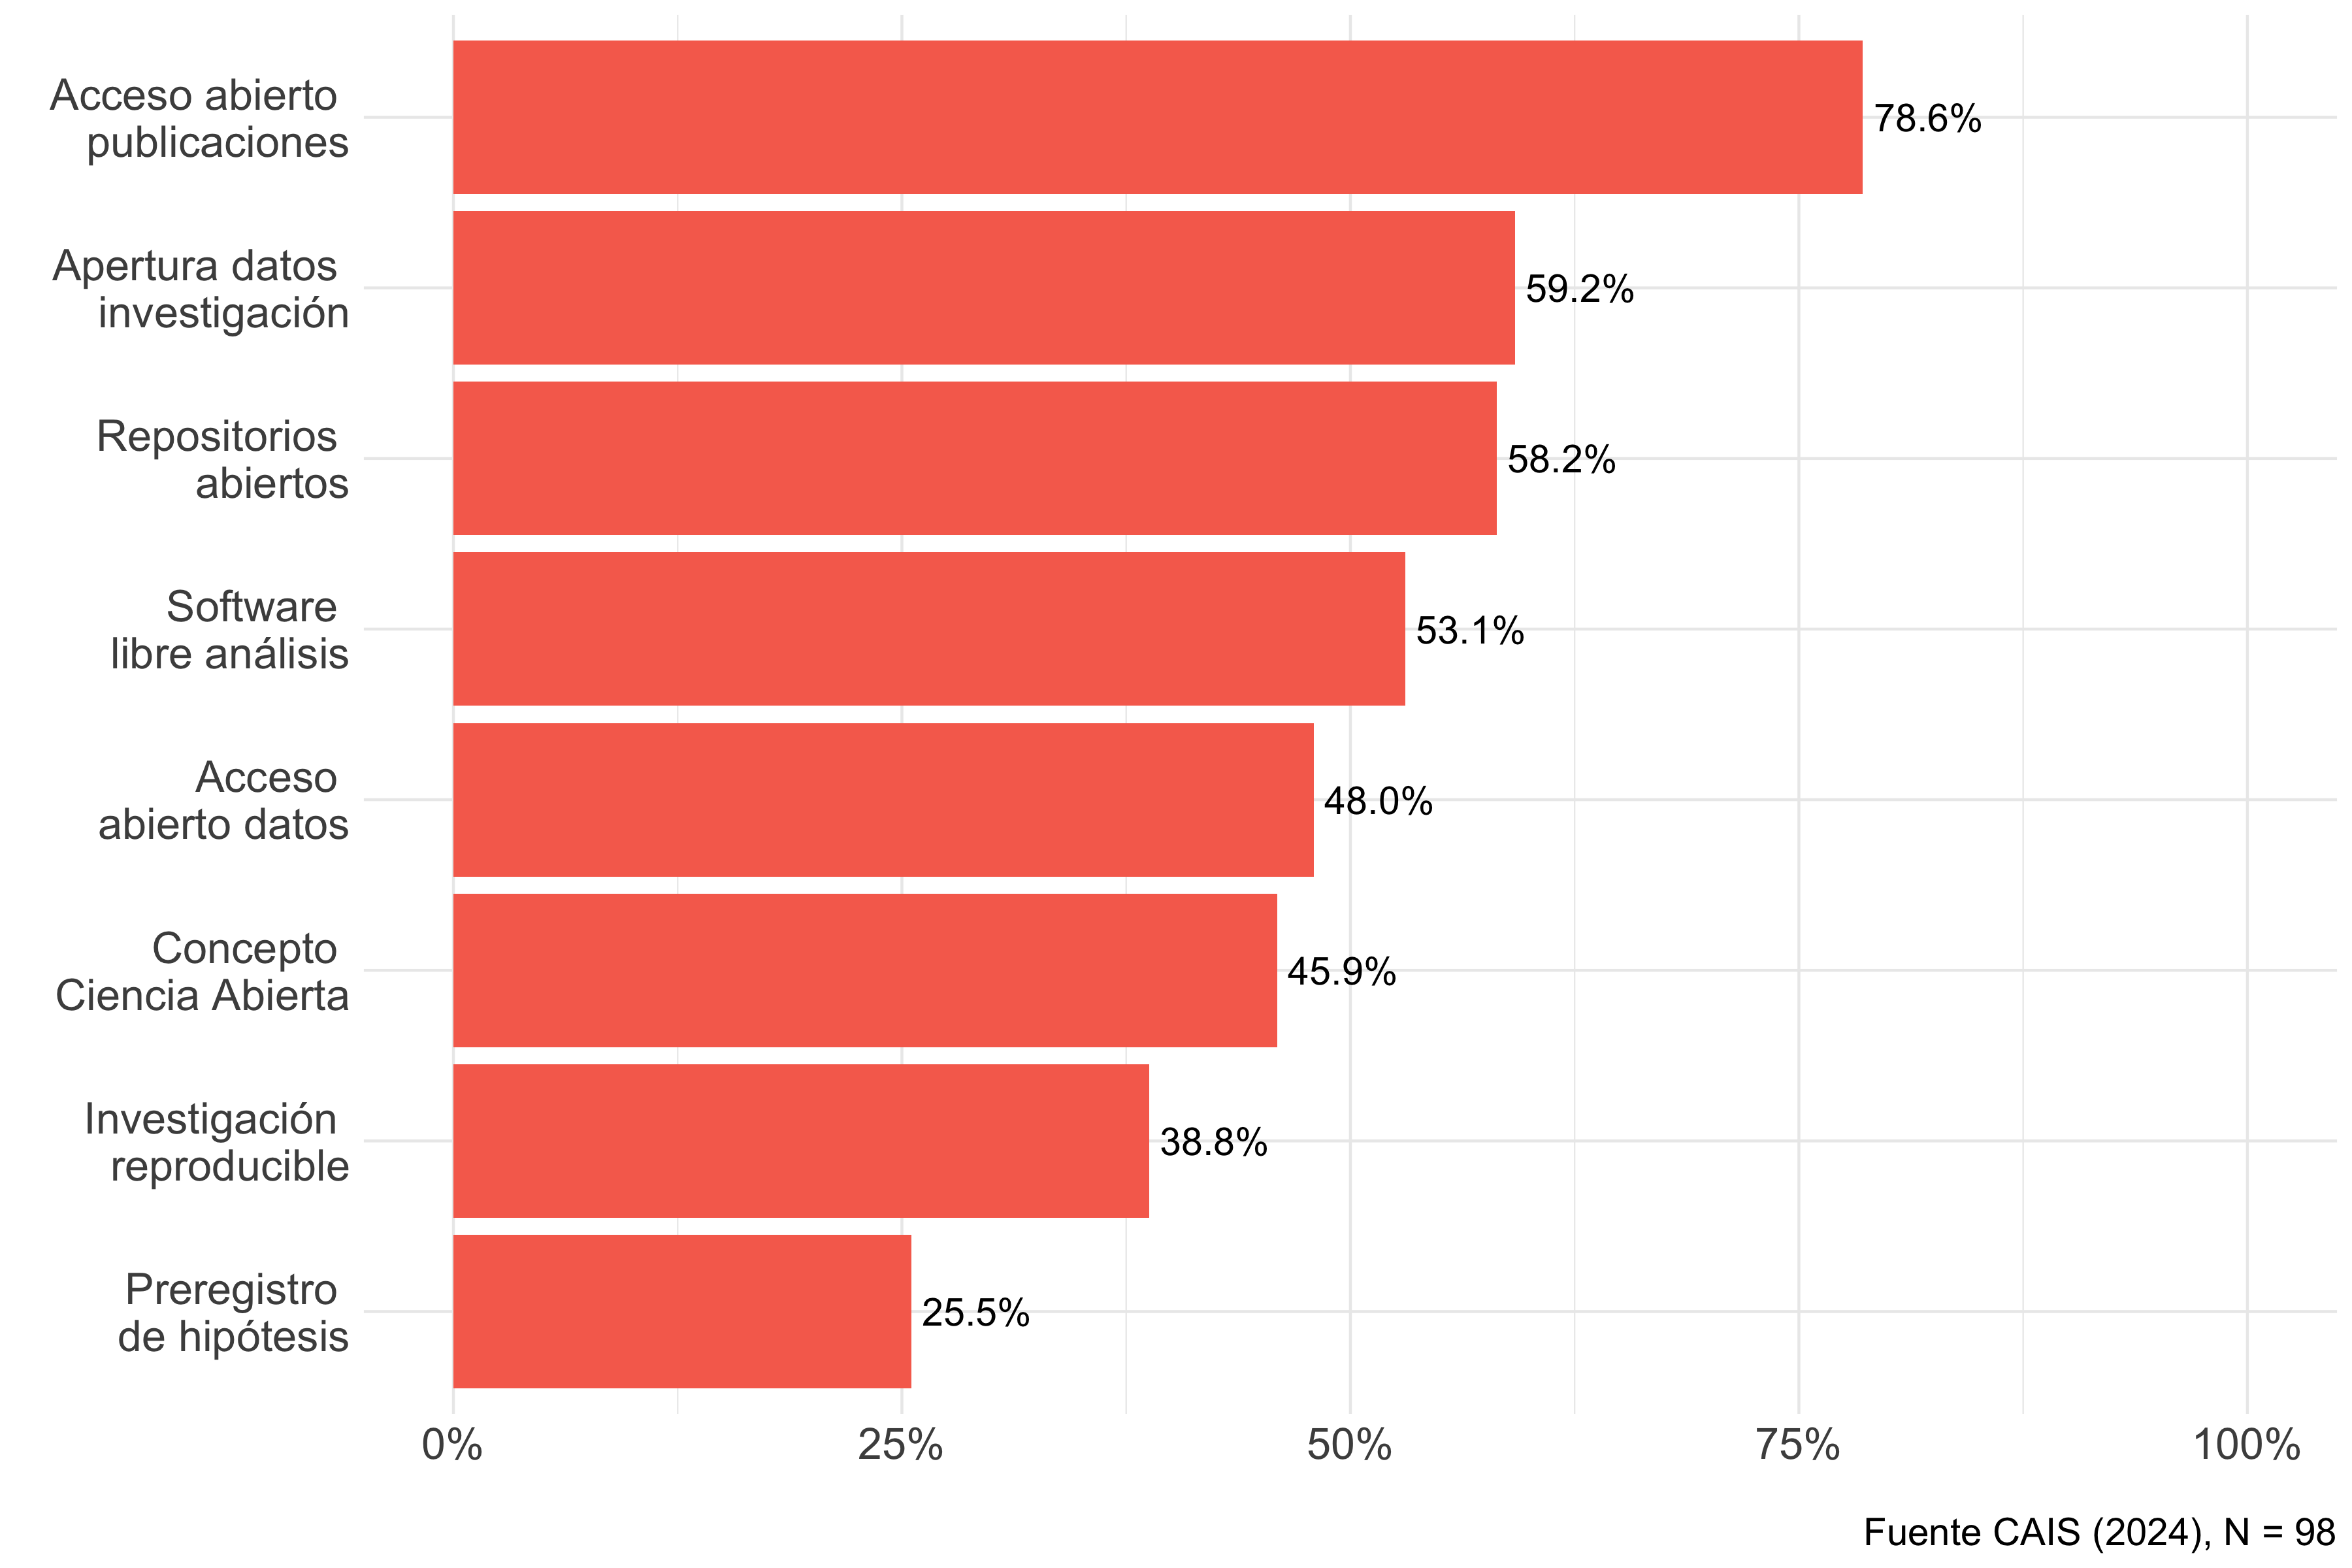
\includegraphics{paper_files/figure-pdf/fig-cca-1.png}

}

\caption{\label{fig-cca}Familiaridad Conceptos de Ciencia Abierta}

\end{figure}

En general, los niveles de conocimiento parecen ser mayores entre
investigadores jóvenes y con enfoque predominantemente cuantitativo,
como se expone en la Figura~\ref{fig-cca-grid}. Los encuestados entre 28
y 34 años, así, muestran mayores niveles de conocimiento sobre softwares
libres, y los conceptos de investigación reproducible y ciencia abierta
(Figura~\ref{fig-cca-grid-1}). Con todo, los investigadores entre 35 y
49 años muestran mayores niveles de conocimiento de los preregistros de
hipótesis y del acceso abierto a datos. Los investigadores
cuantitativos, en tanto, presentan mayores niveles de conocimiento de
todos los conceptos, salvo en el acceso abierto a publicaciones
(Figura~\ref{fig-cca-grid-2}).

\begin{figure}

\begin{minipage}[t]{\linewidth}

{\centering 

\raisebox{-\height}{

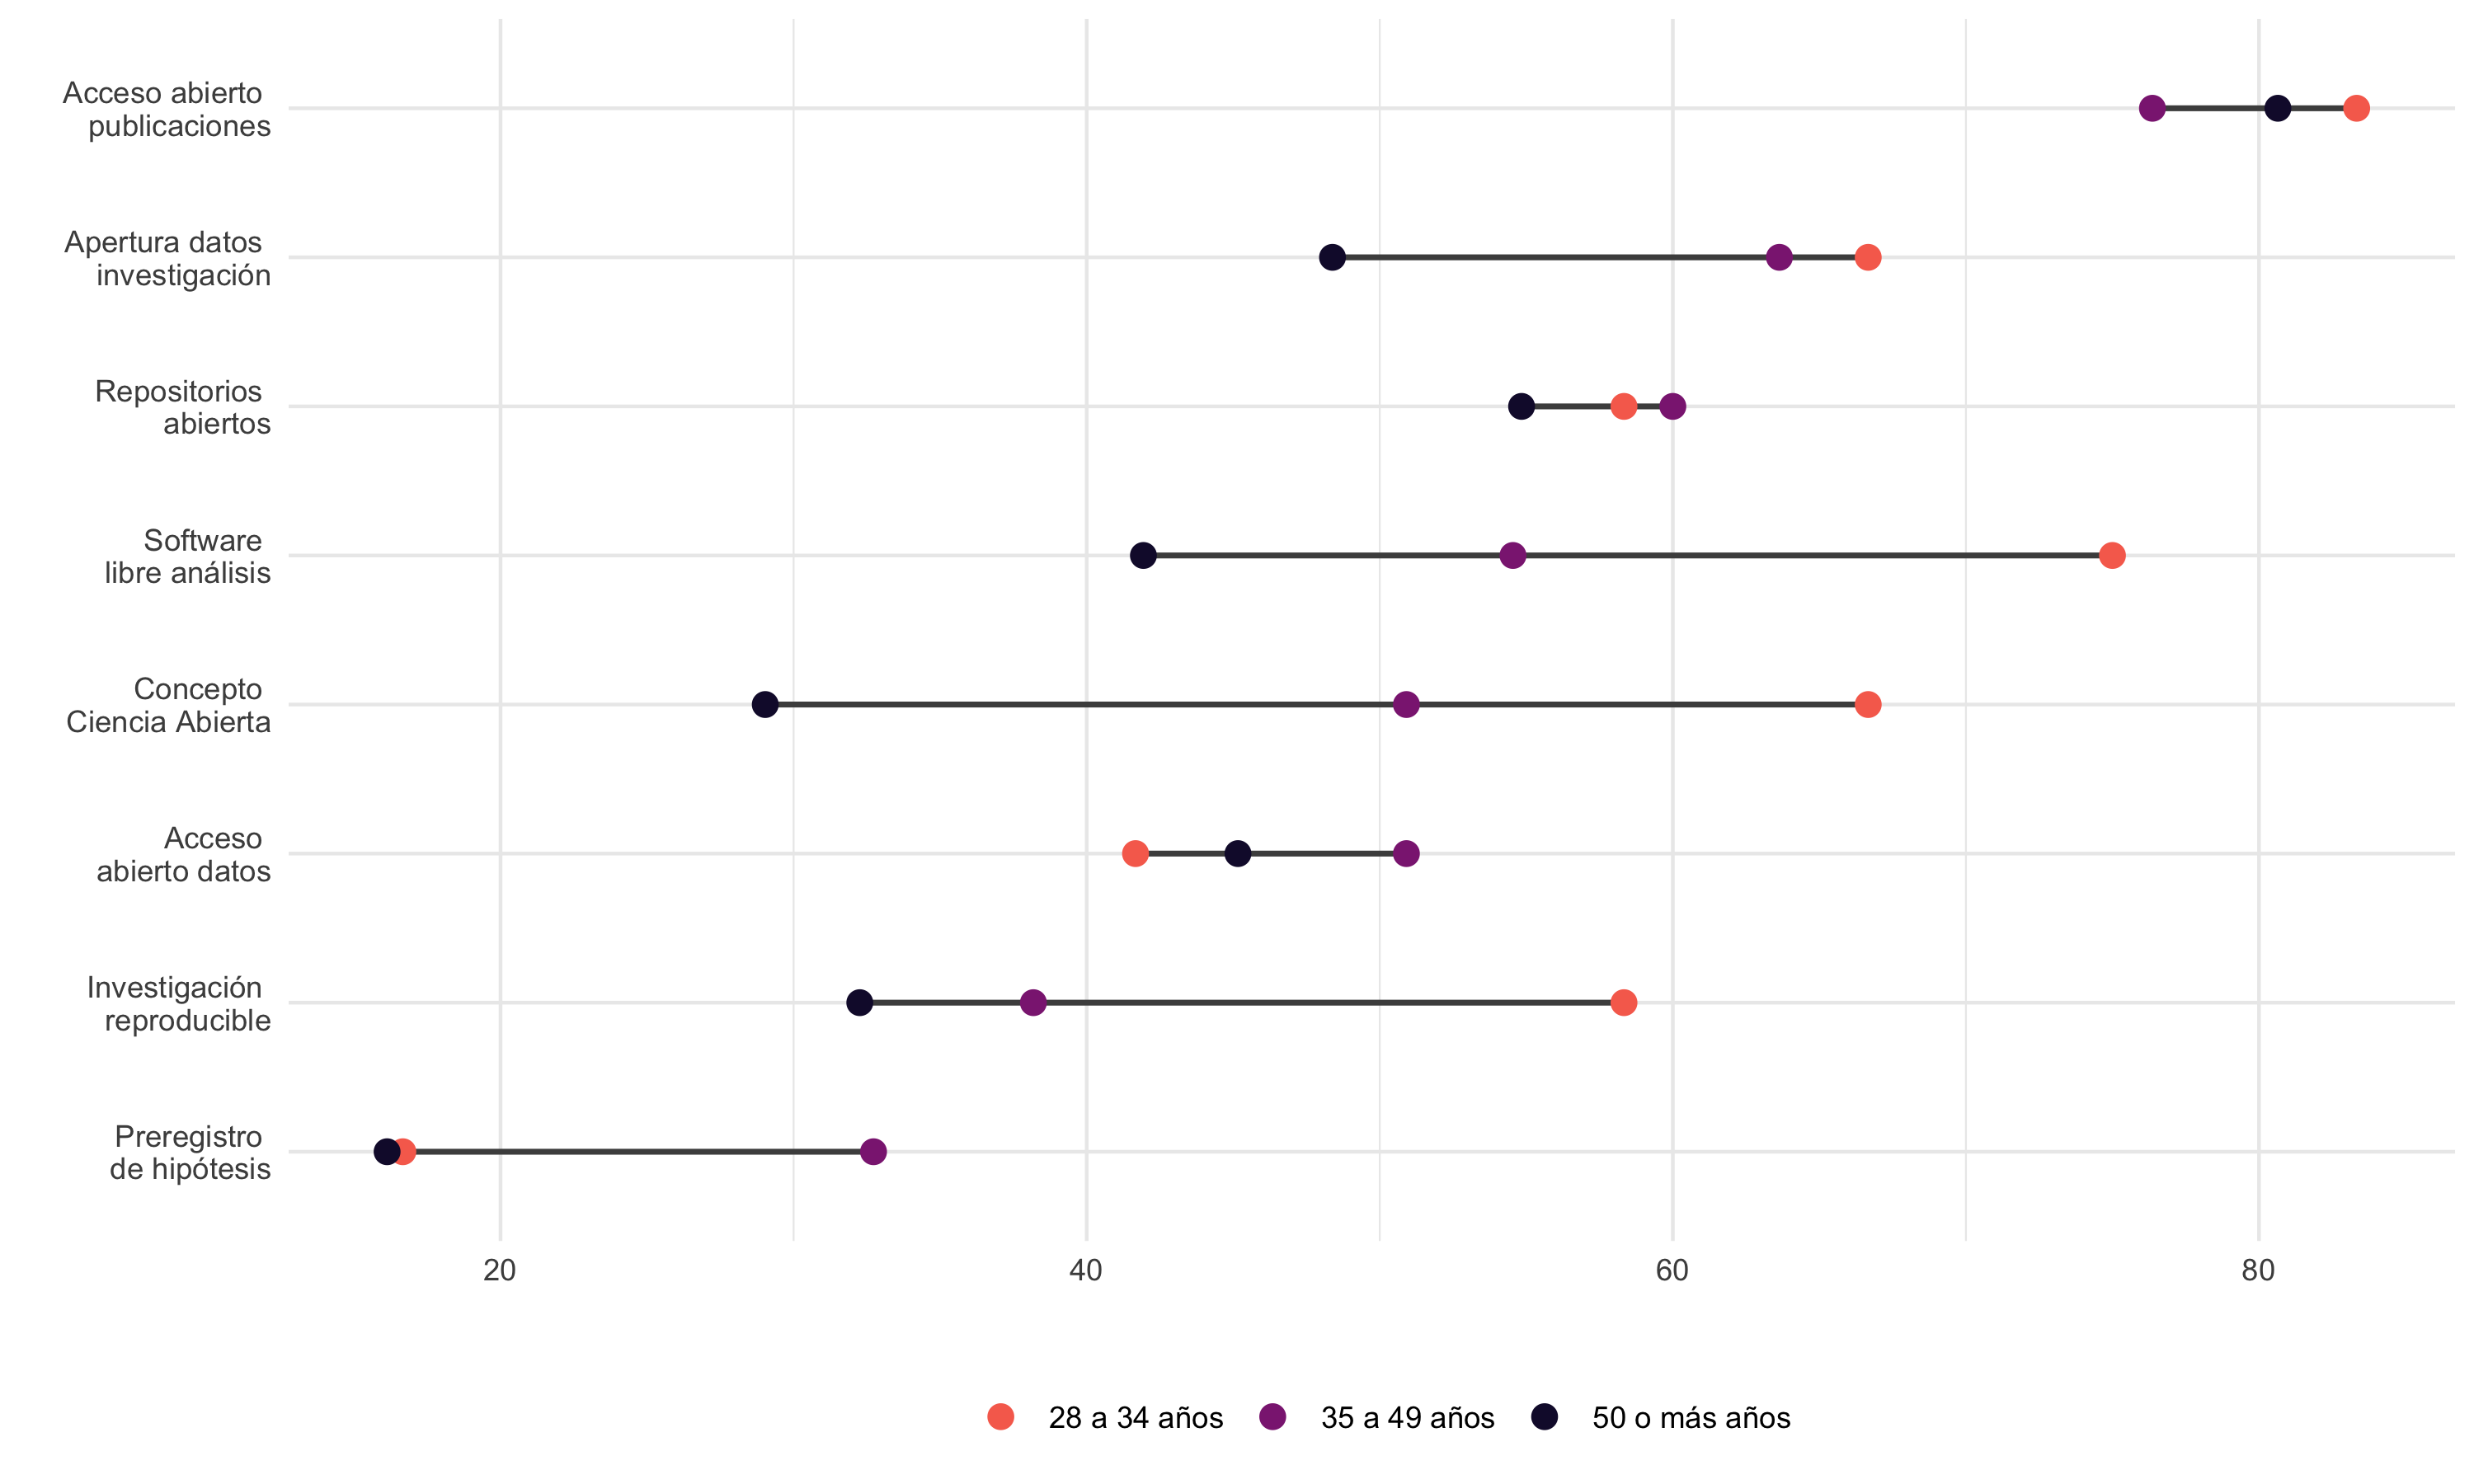
\includegraphics{paper_files/figure-pdf/fig-cca-grid-1.png}

}

}

\subcaption{\label{fig-cca-grid-1}Familiaridad conceptos ciencia abierta
por edad}
\end{minipage}%
\newline
\begin{minipage}[t]{\linewidth}

{\centering 

\raisebox{-\height}{

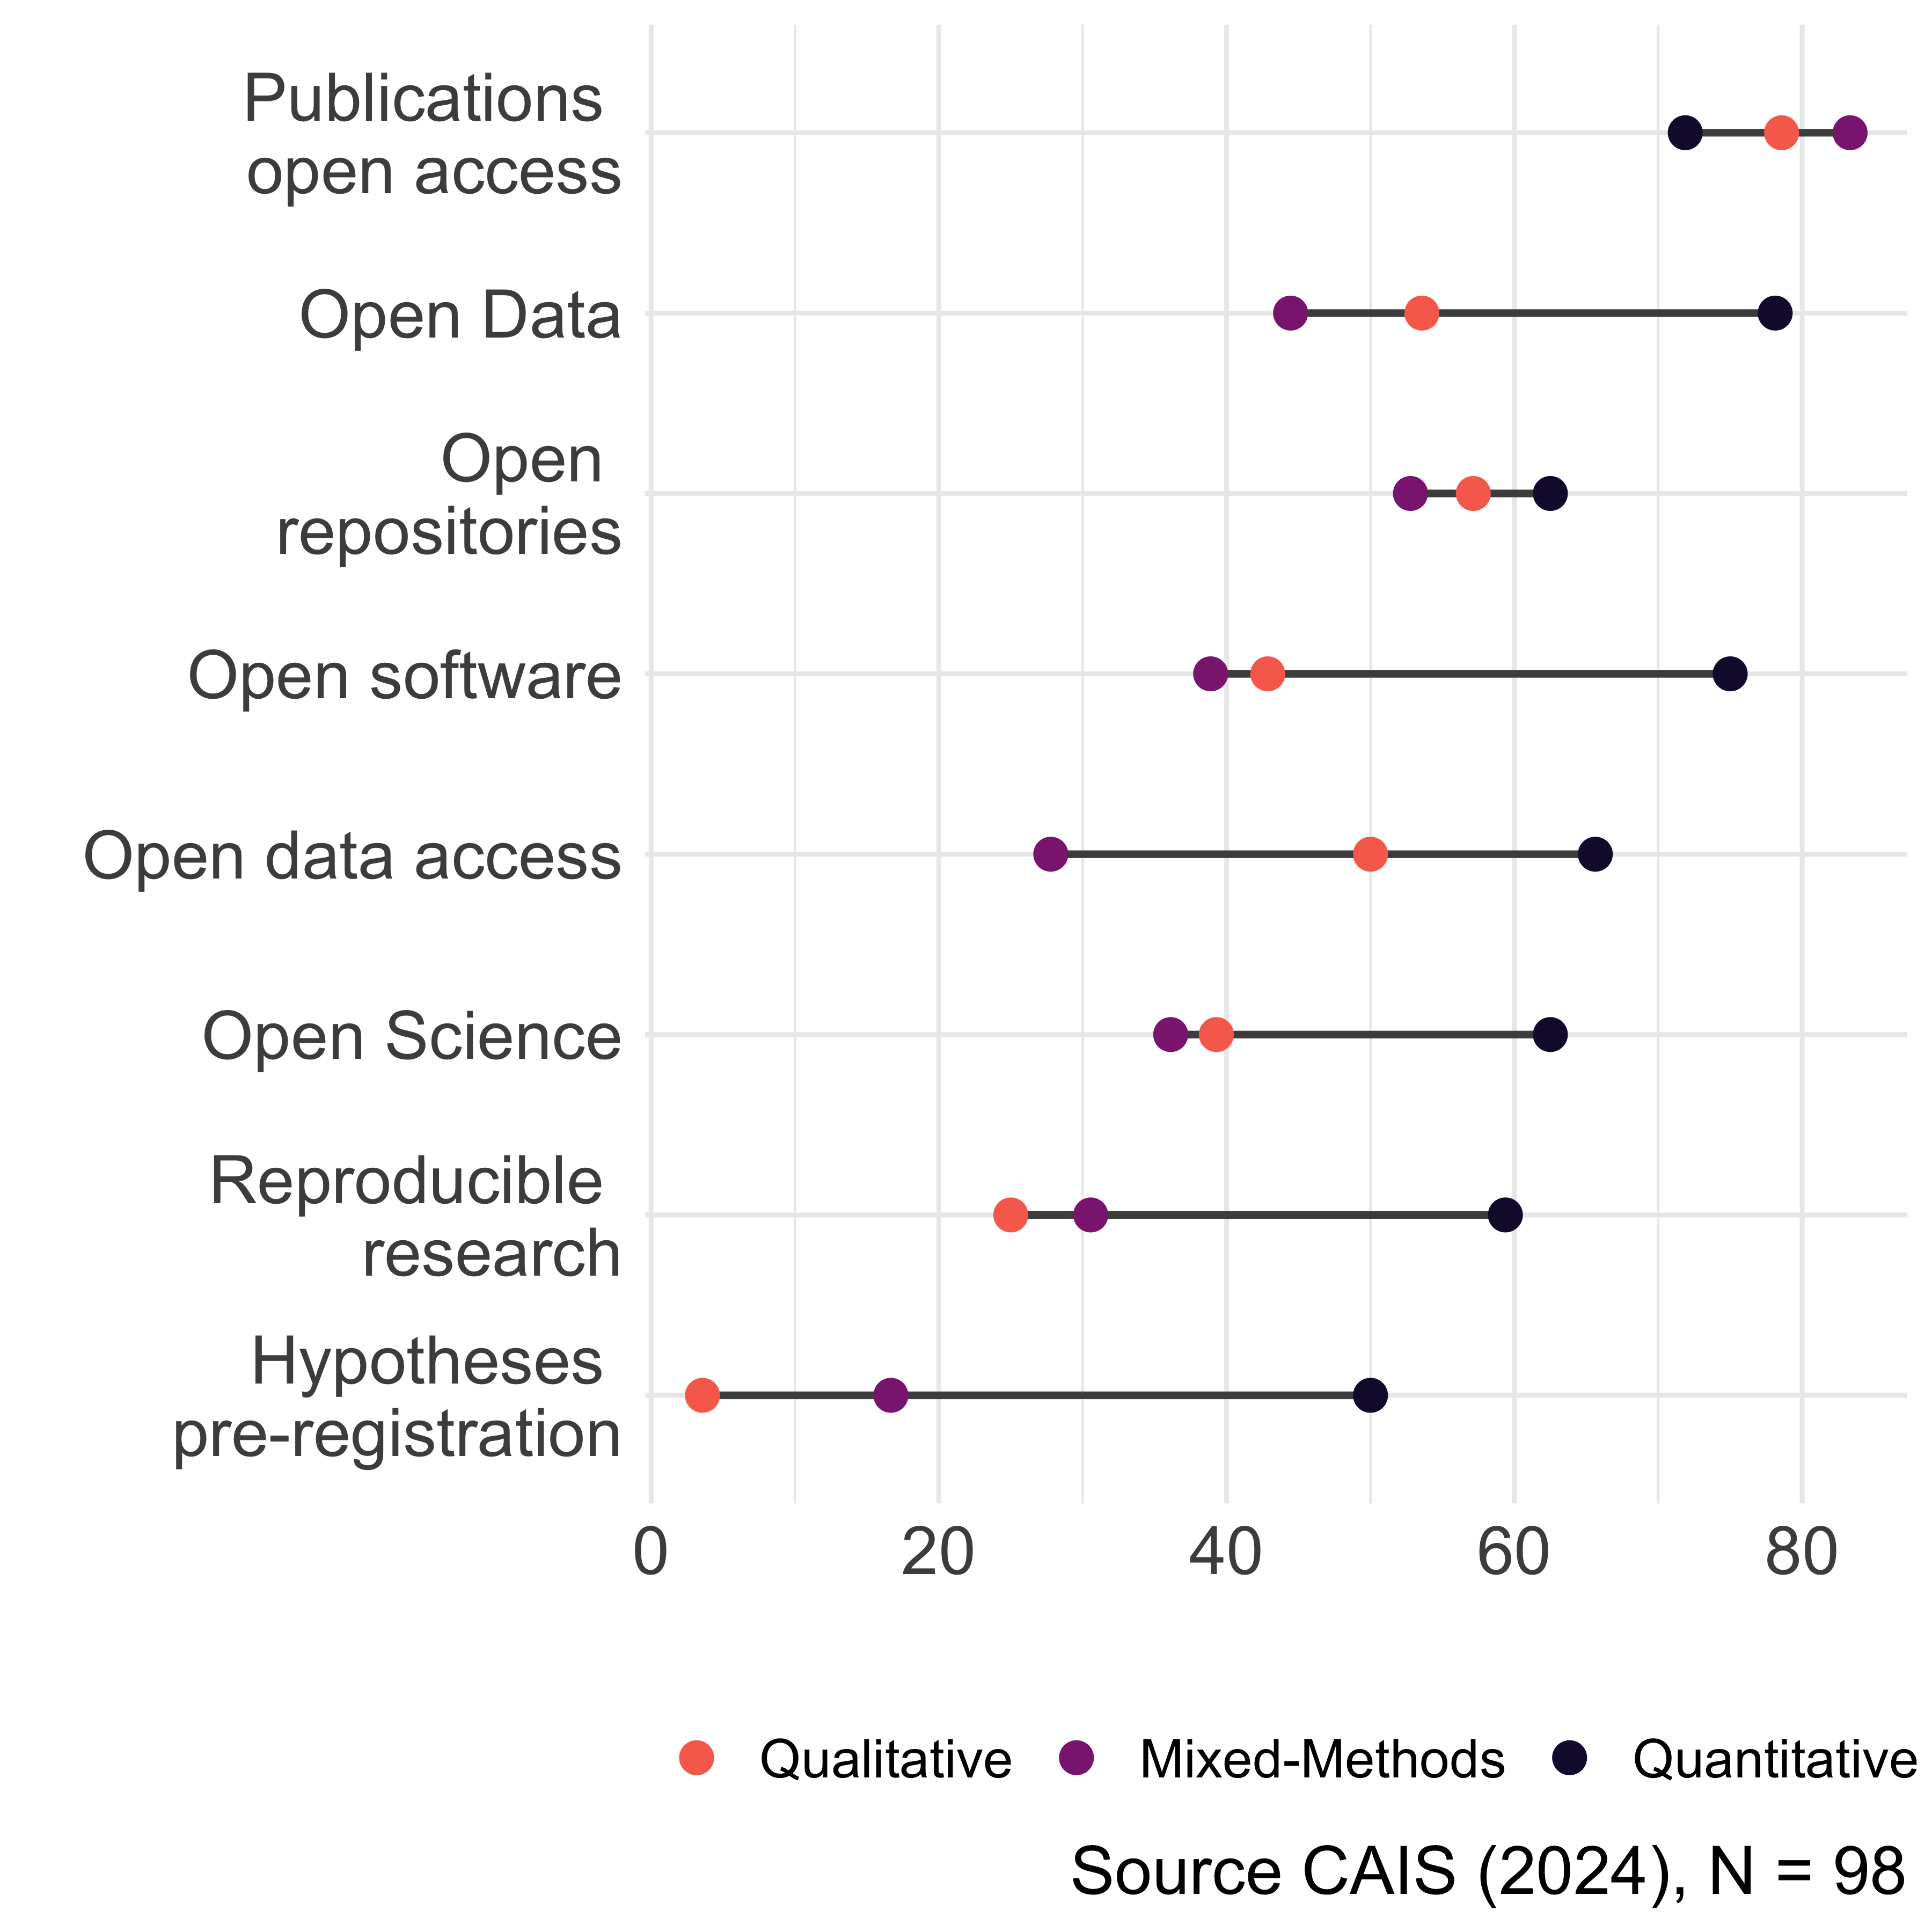
\includegraphics{paper_files/figure-pdf/fig-cca-grid-2.png}

}

}

\subcaption{\label{fig-cca-grid-2}Familiaridad conceptos ciencia abierta
por enfoque}
\end{minipage}%

\caption{\label{fig-cca-grid}Familiaridad conceptos ciencia abierta por
edad y enfoque de investigación}

\end{figure}

En la misma línea, La Política de Acceso Abierto a la Información
Científica y a Datos de Investigación muestra niveles de conocimiento de
intermedios a bajo. En concreto, solo la mitad de los encuestados han
escuchado hablar sobre la política de acceso abierto de la ANID. Por
otro lado, solo un 26\% conoce el plan de gestión de datos de la
política de acceso abierto de la ANID.

\textbf{Prácticas}

\begin{enumerate}
\def\labelenumi{\alph{enumi})}
\tightlist
\item
  Práctica propias y prácticas de la comunidad
\end{enumerate}

En general, se observa una baja frecuencia de prácticas relacionadas con
la ciencia abierta, como se aprecia en Figura~\ref{fig-prac}. Un 32\% de
los encuestados siempre o casi siempre utiliza repositorios en línea
para subir información relacionada a sus investigaciones, y un 16\%
declara compartir códigos entre investigadores
(Figura~\ref{fig-prac-2}). Este tipo de prácticas son más comunes entre
investigadores hombres, aquellos cuyo enfoque predominante es
cuantitativo, y quienes están en una etapa inicial de su carrera
académica.

\begin{figure}

\begin{minipage}[t]{\linewidth}

{\centering 

\raisebox{-\height}{

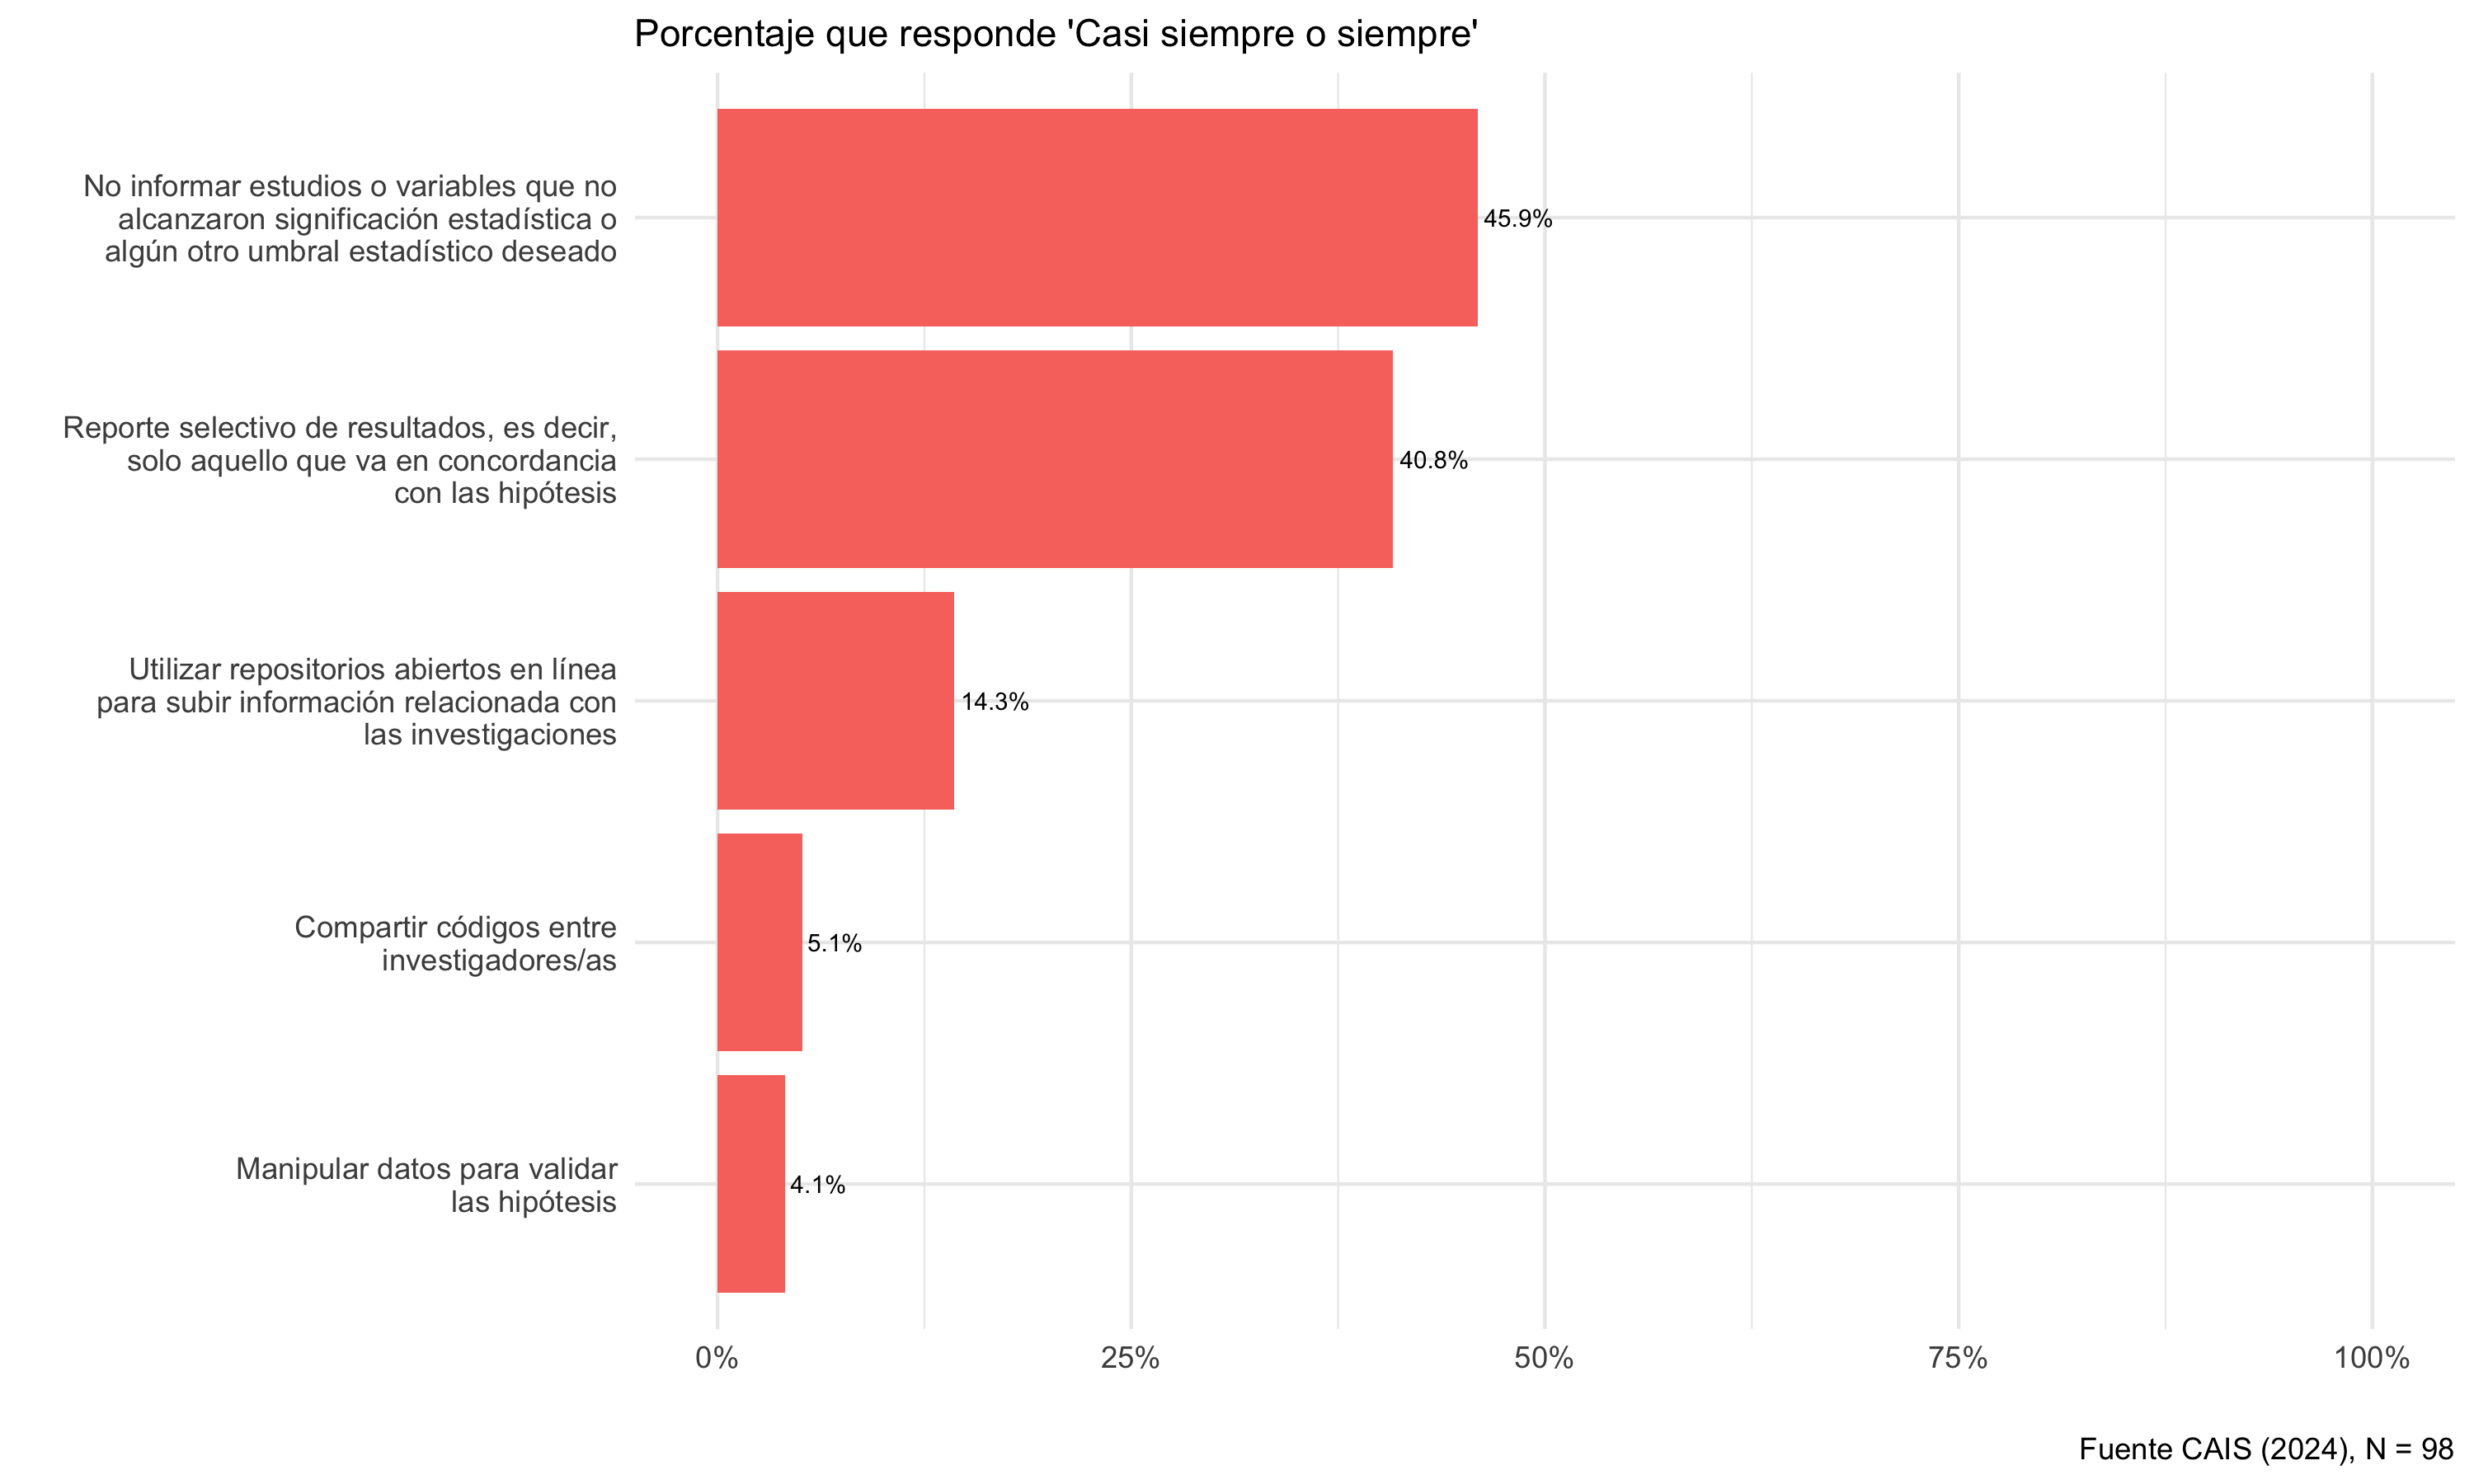
\includegraphics{paper_files/figure-pdf/fig-prac-1.png}

}

}

\subcaption{\label{fig-prac-1}Prácticas de la Comunidad}
\end{minipage}%
\newline
\begin{minipage}[t]{\linewidth}

{\centering 

\raisebox{-\height}{

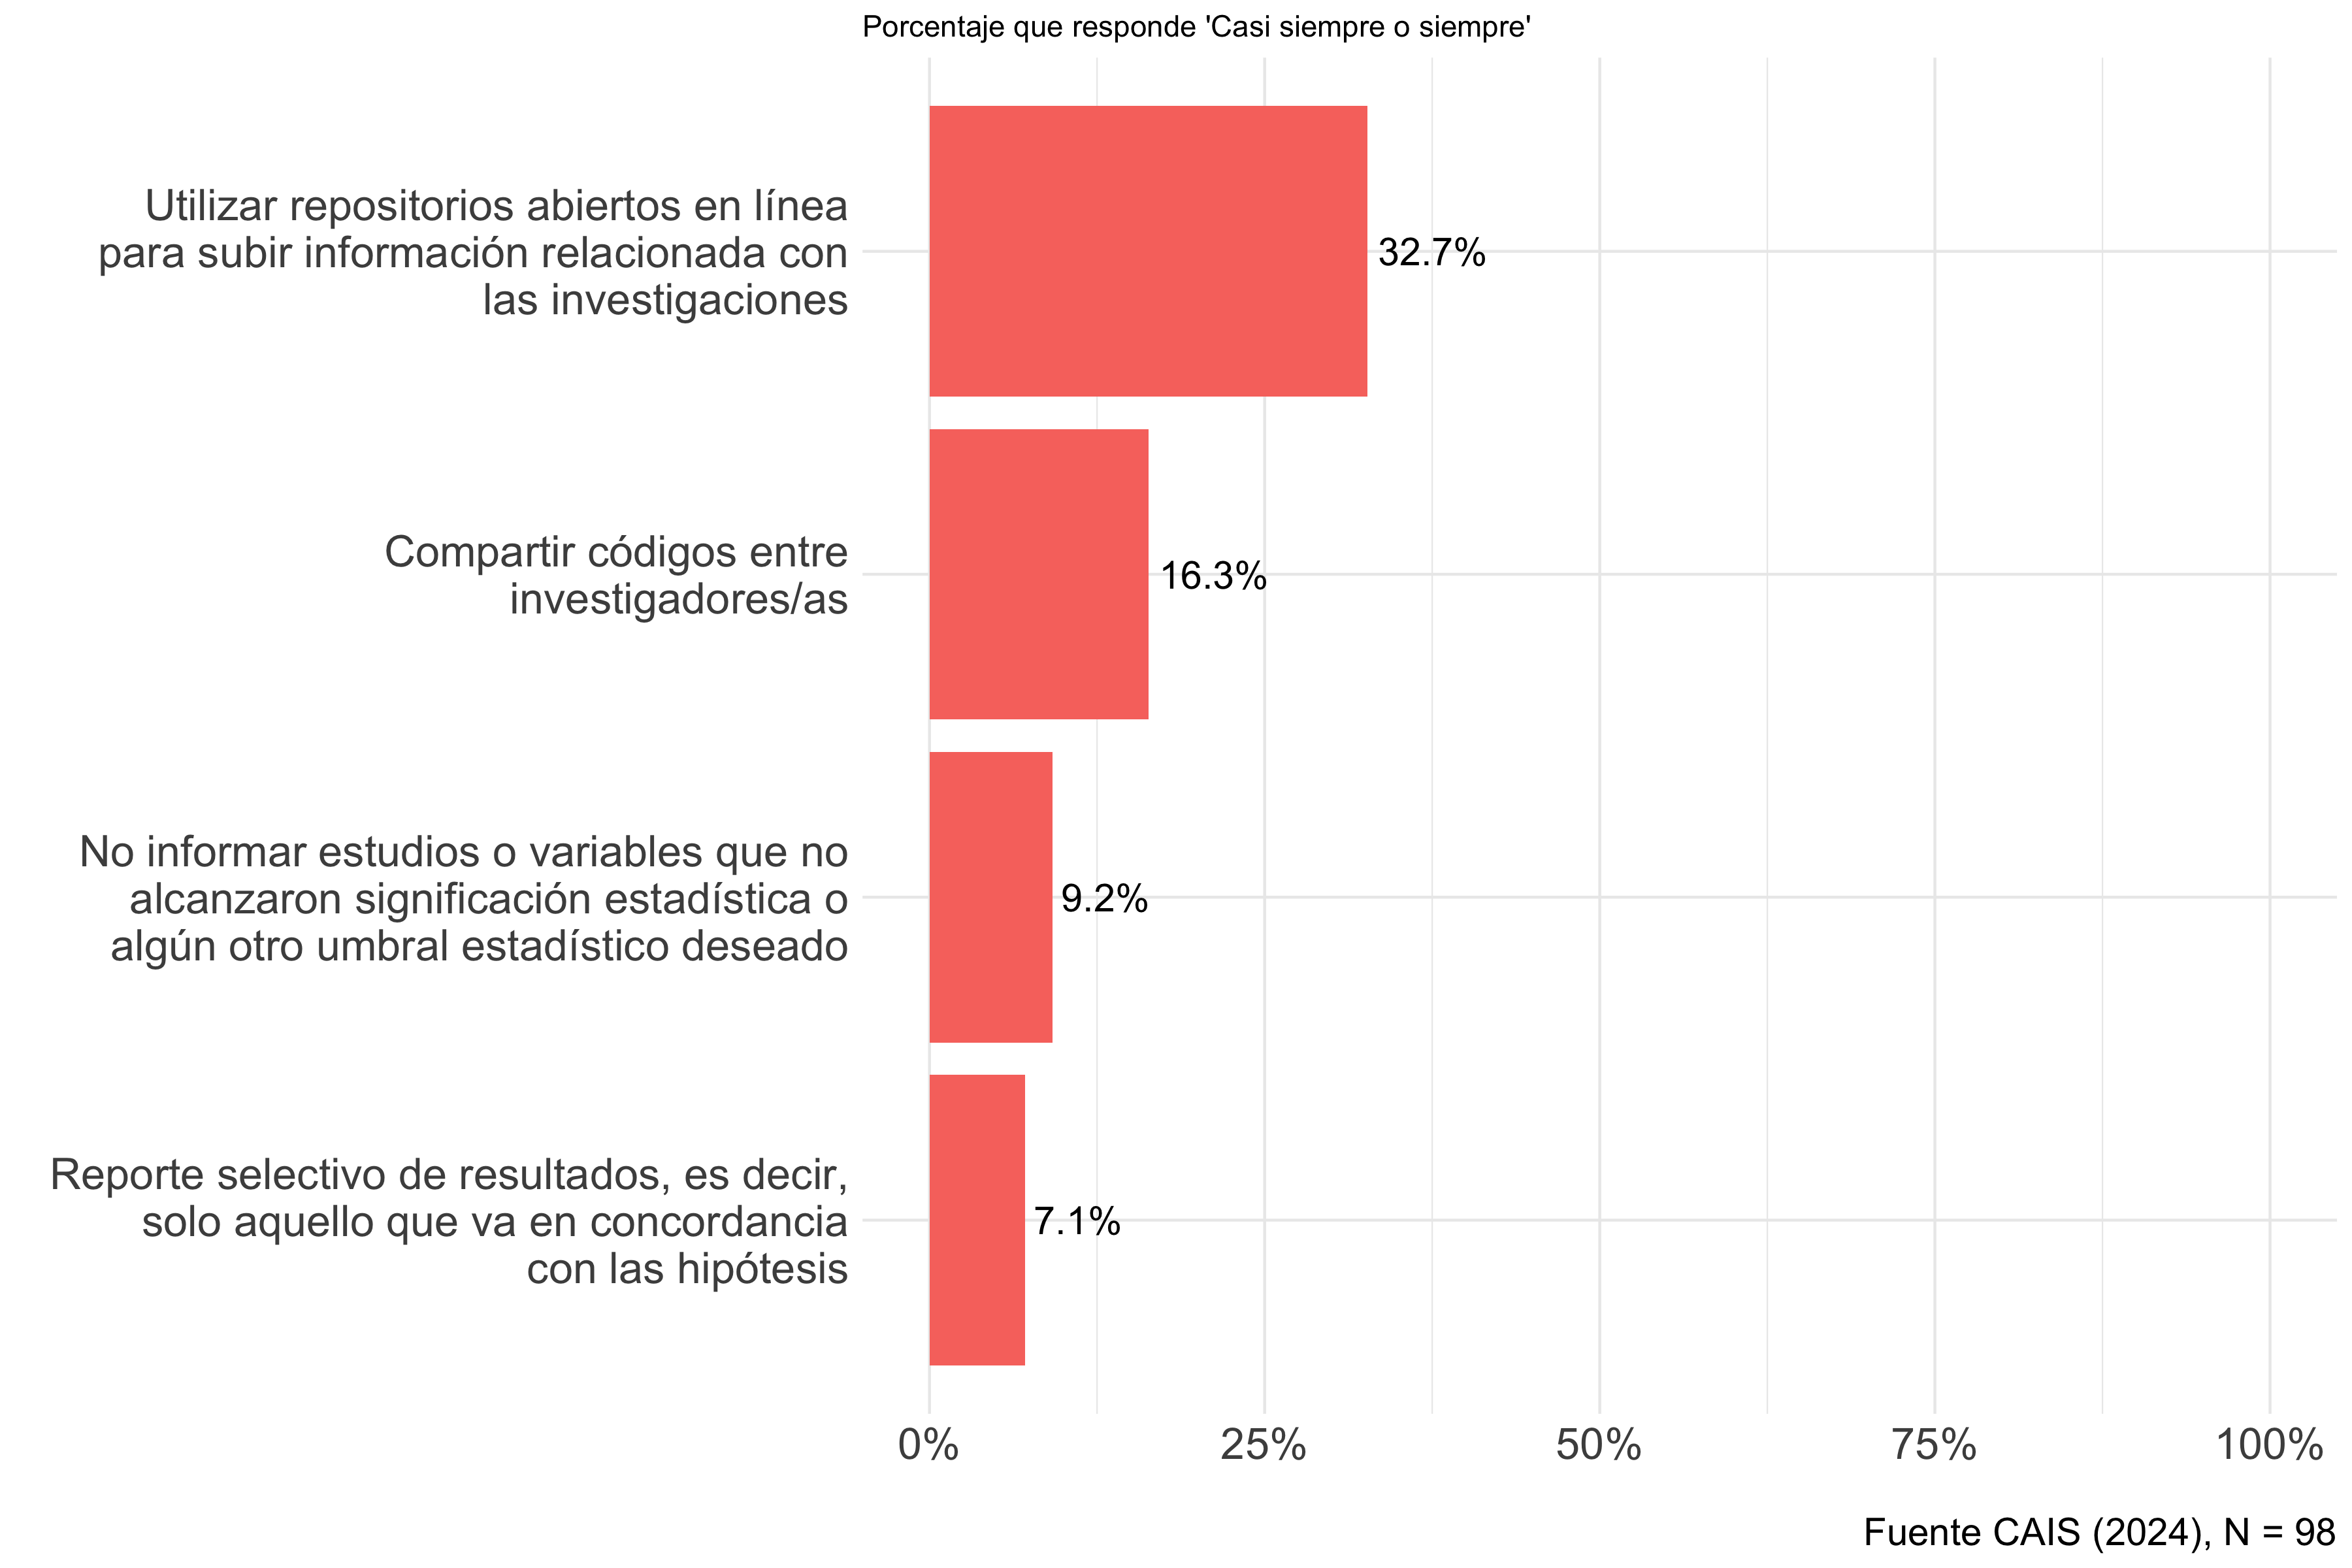
\includegraphics{paper_files/figure-pdf/fig-prac-2.png}

}

}

\subcaption{\label{fig-prac-2}Prácticas propias}
\end{minipage}%

\caption{\label{fig-prac}¿Con qué frecuencias se realizan las siguientes
prácticas?}

\end{figure}

Es interesante que, en general, los investigadores declaran mejores
prácticas propias que las percibidas en la comunidad. De tal modo, sólo
un 14\% cree que siempre o casi siempre la comunidad utiliza
repositorios en línea para subir información relacionada a sus
investigaciones, y un 5\% cree que los investigadores comparten códigos
con esa frecuencia (Figura~\ref{fig-prac-1}).

Esta brecha es cierta también en lo relativo a las malas prácticas. Un
9\% de los encuestados declara que casi siempre o siempre no informa
estudios o variables que no alcanzaron significación estadística,
mientras que un 45\% percibe esta práctica como frecuente en la
comunidad. Por otro lado, mientras un 7\% declara reportar
selectivamente resultados, el 40\% cree que esto ocurre siempre o casi
siempre entre la comunidad. Finalmente, mientras nadie reconoce
manipular datos para validar una hipótesis, el 4\% afirma que esto
ocurre siempre o casi siempre en la comunidad.

Es curioso que al desagregar el análisis en distintos grupos, se repiten
ciertas tendencias: Los investigadores hombres, de enfoque cuantitativo
y de carrera inicial son, al mismo tiempo, quienes reconocen mayor
frecuencia de prácticas propias, tanto negativas como positivas, como
quienes perciben la mayor cantidad de prácticas negativas en la
comunidad. Estas diferencias se pueden ver en detalle en
Figura~\ref{fig-prac-grid}

\begin{figure}

\begin{minipage}[t]{\linewidth}

{\centering 

\raisebox{-\height}{

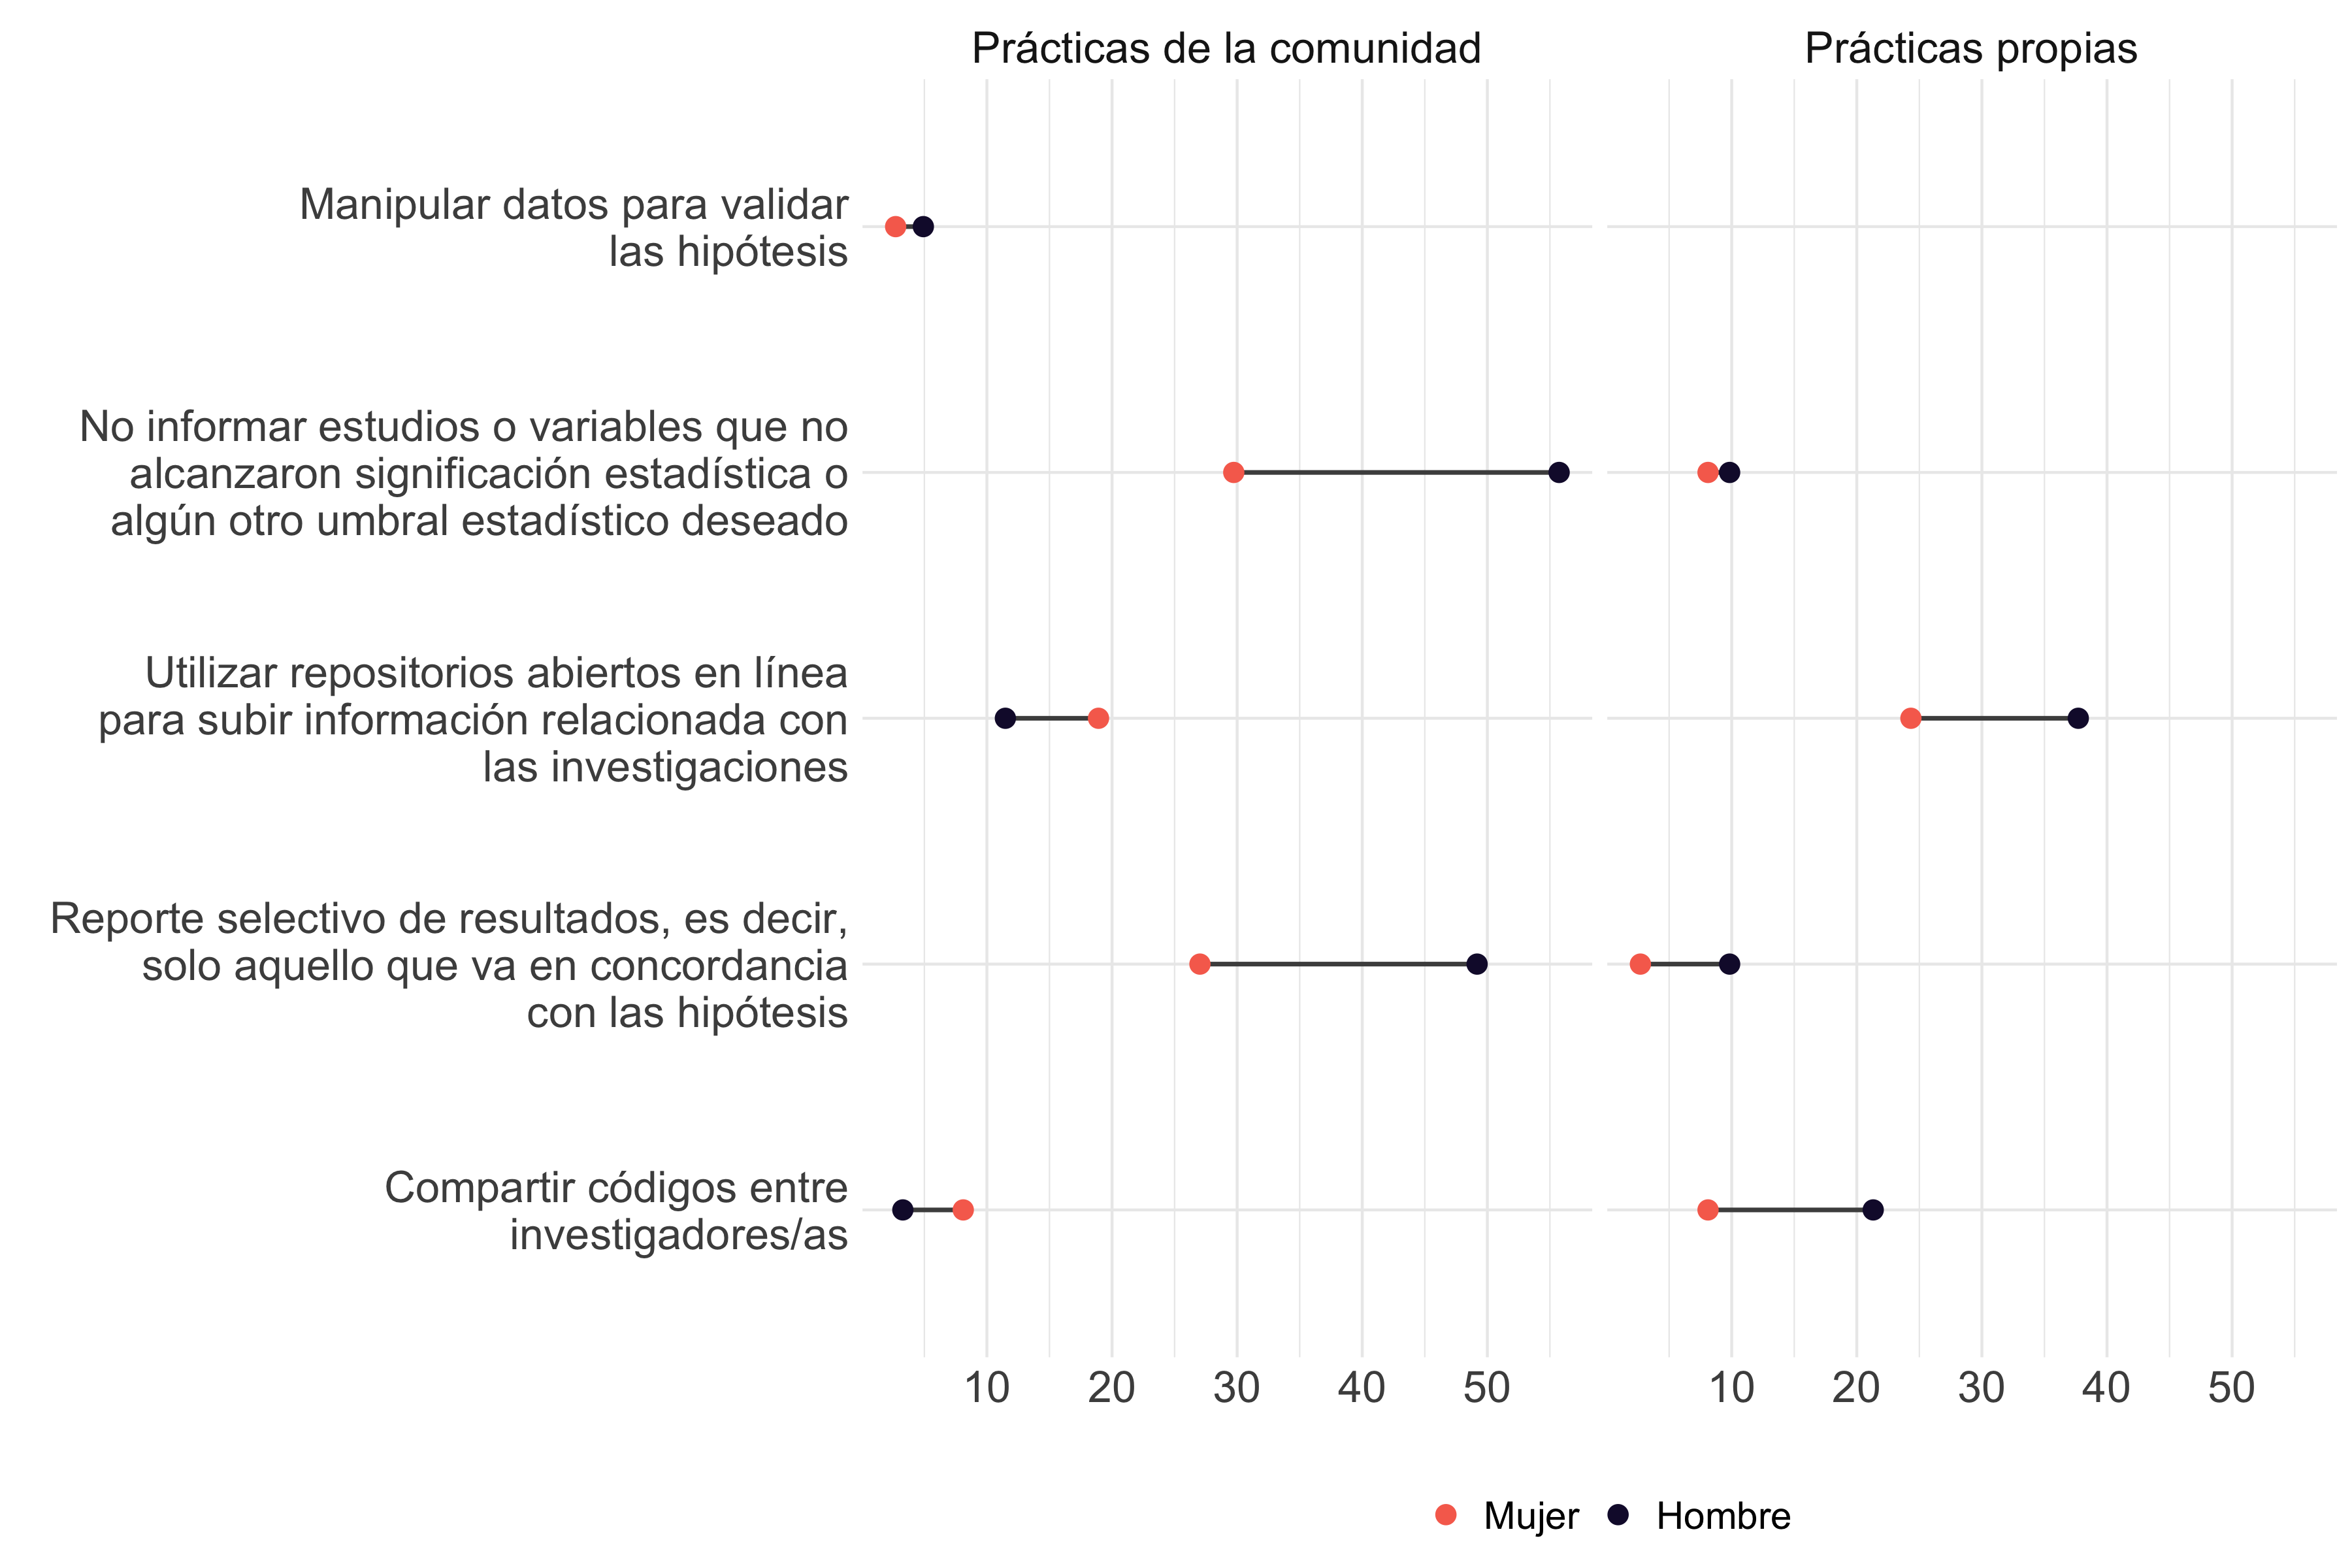
\includegraphics{paper_files/figure-pdf/fig-prac-grid-1.png}

}

}

\subcaption{\label{fig-prac-grid-1}Por sexo}
\end{minipage}%
\newline
\begin{minipage}[t]{\linewidth}

{\centering 

\raisebox{-\height}{

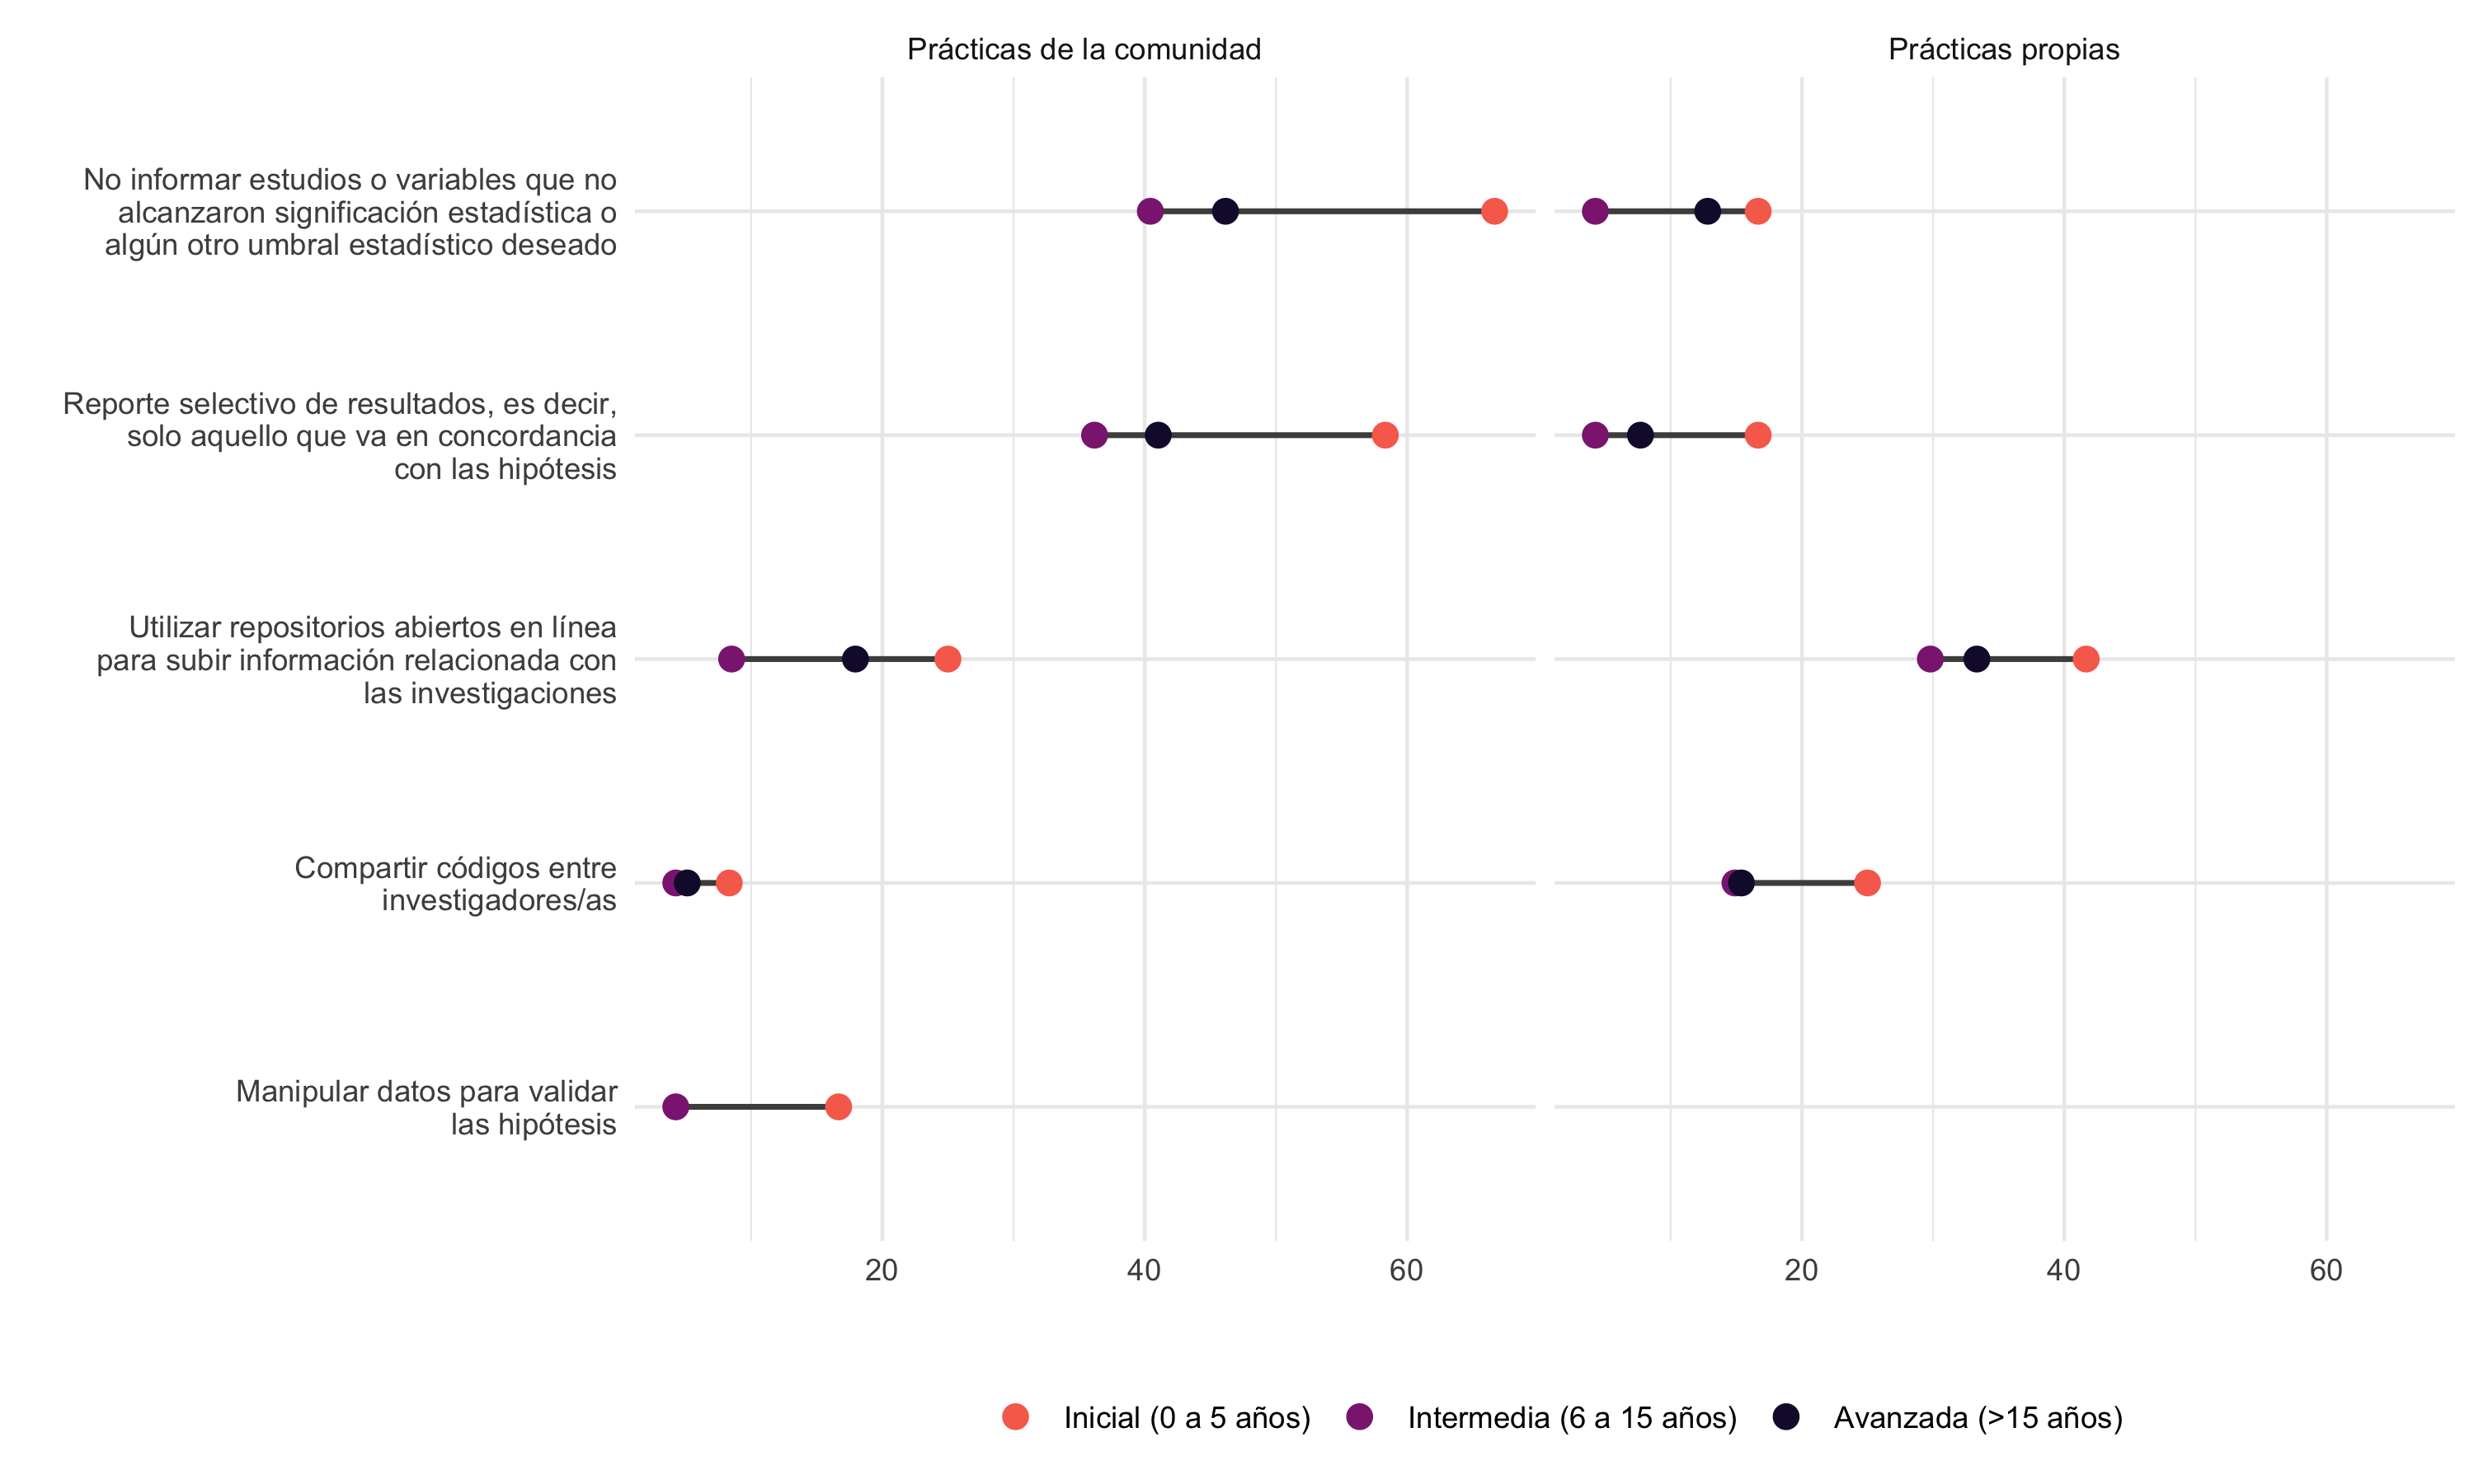
\includegraphics{paper_files/figure-pdf/fig-prac-grid-2.png}

}

}

\subcaption{\label{fig-prac-grid-2}Por etapa en la carrera académica}
\end{minipage}%
\newline
\begin{minipage}[t]{\linewidth}

{\centering 

\raisebox{-\height}{

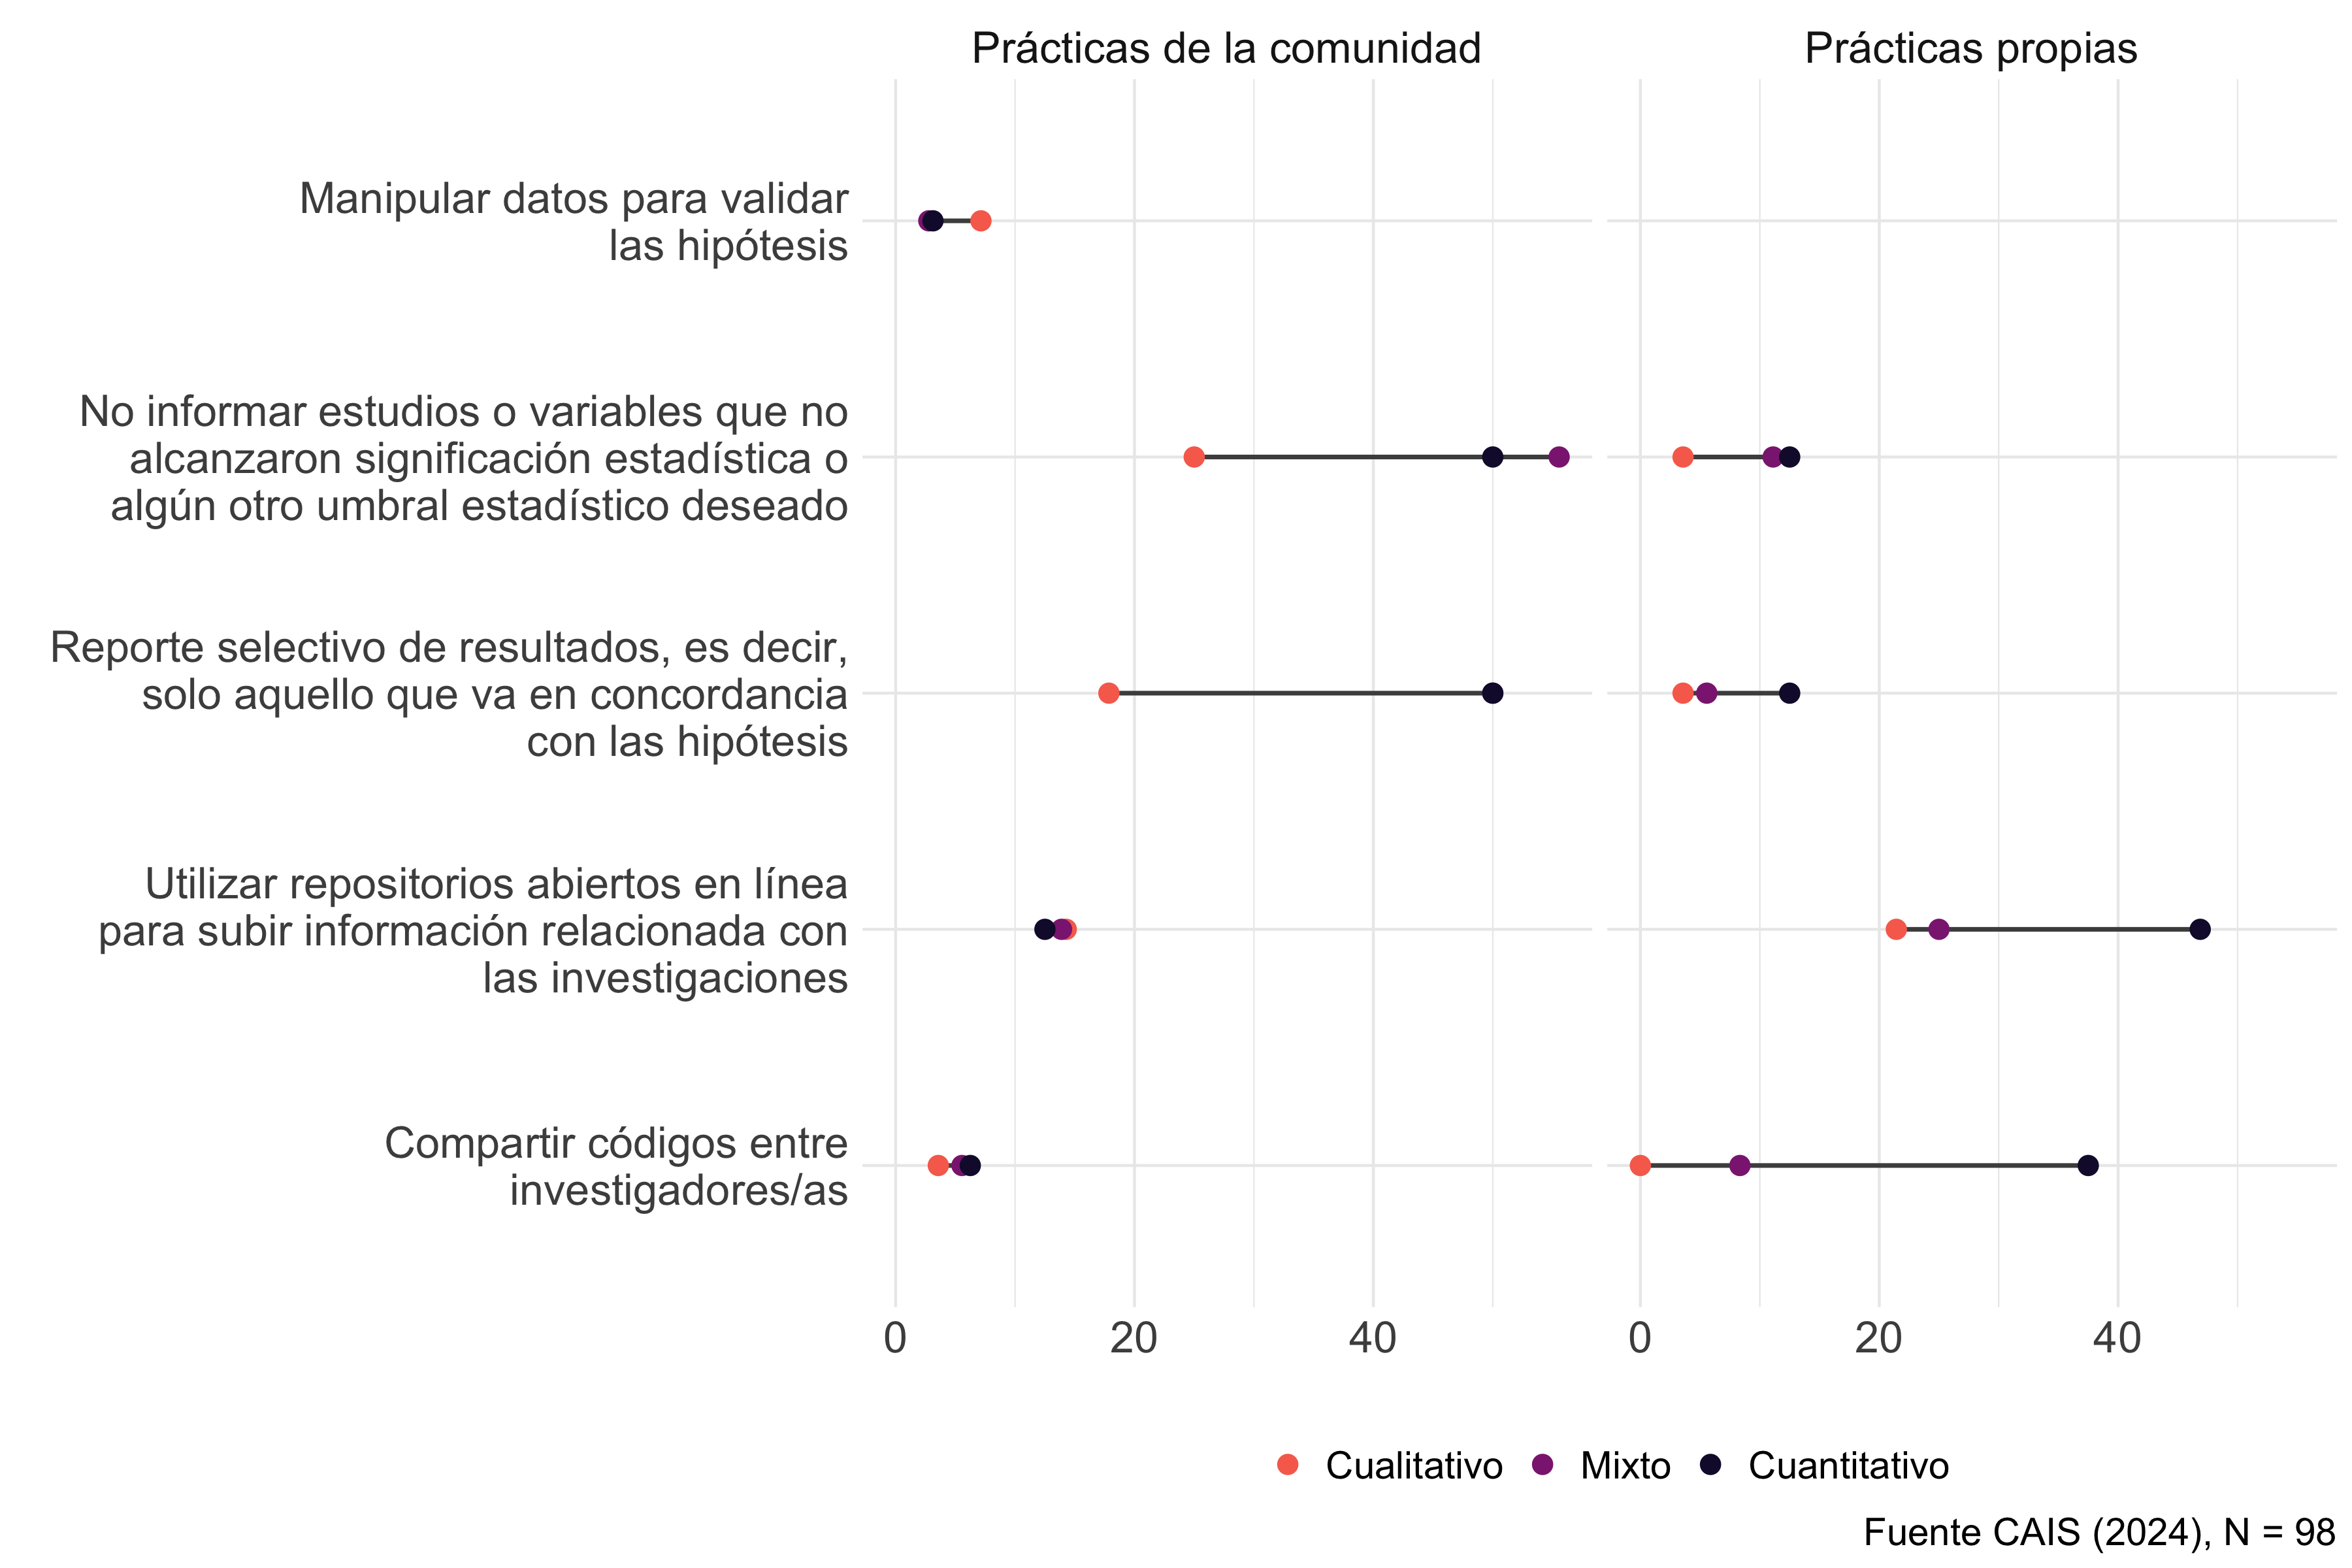
\includegraphics{paper_files/figure-pdf/fig-prac-grid-3.png}

}

}

\subcaption{\label{fig-prac-grid-3}Por enfoque de investigación}
\end{minipage}%

\caption{\label{fig-prac-grid}¿Con qué frecuencias se realizan las
siguientes prácticas?}

\end{figure}

\begin{enumerate}
\def\labelenumi{\alph{enumi})}
\setcounter{enumi}{1}
\tightlist
\item
  Barreras para la Ciencia Abierta
\end{enumerate}

Por otro lado, se observa una alta percepción de barreras para el
desarrollo de la ciencia abierta en todas sus dimensiones. La Falta de
políticas es reconocida como la principal barrera en todas las
dimensiones, como se puede apreciar en la Figura~\ref{fig-barreras}. La
falta de conocimientos también aparece como una barrera importante,
particularmente para el diseño transparente, la apertura de datos y la
investigación reproducible. Por último, la falta de incentivos es
reconocida como otro aspecto que dificulta la apertura de datos.

\begin{figure}

{\centering 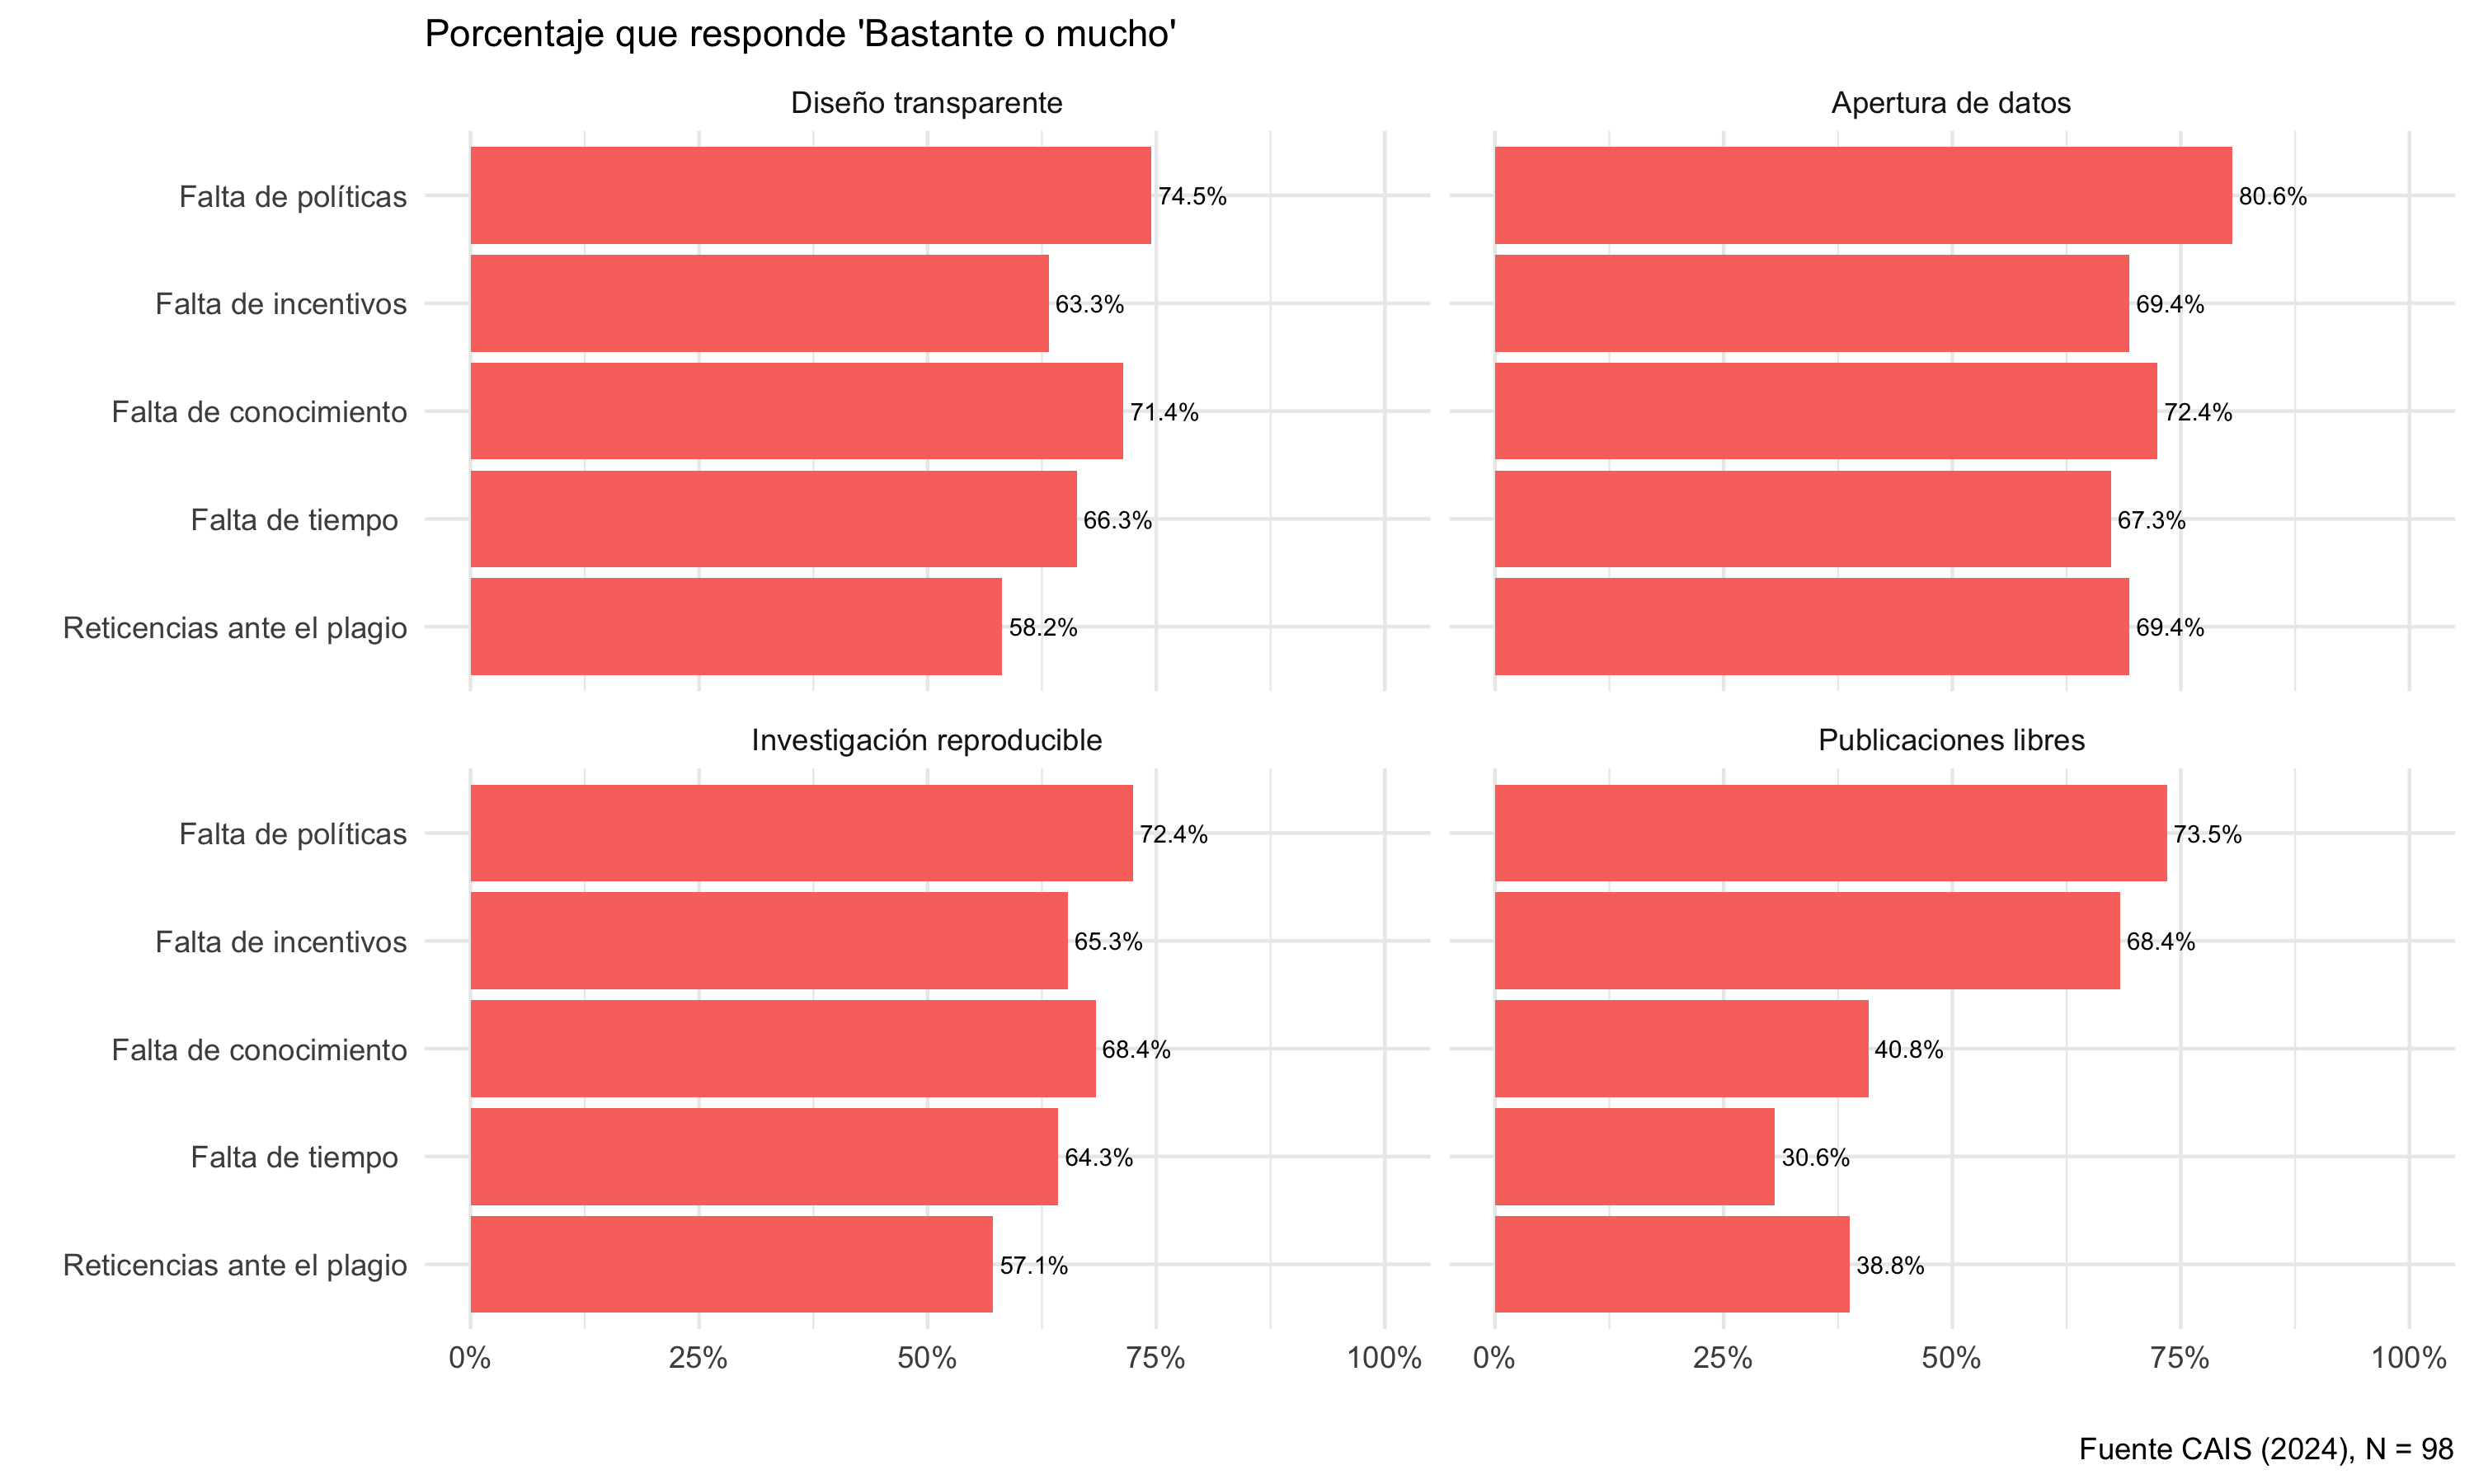
\includegraphics{paper_files/figure-pdf/fig-barreras-1.png}

}

\caption{\label{fig-barreras}¿En qué medida considera que los siguientes
factores limitan la Ciencia Abierta?}

\end{figure}

Respecto a este último punto, se abordaron los incentivos que podrían
tener los investigadores para abrir sus datos. Como se aprecia en la
Figura~\ref{fig-motivaciones}, tanto generar redes, como difundir a la
comunidad datos financiados con recursos públicos y aumentar la
visibilidad propia son altamente valoradas como incentivos para la
apertura de datos.

\begin{figure}

{\centering 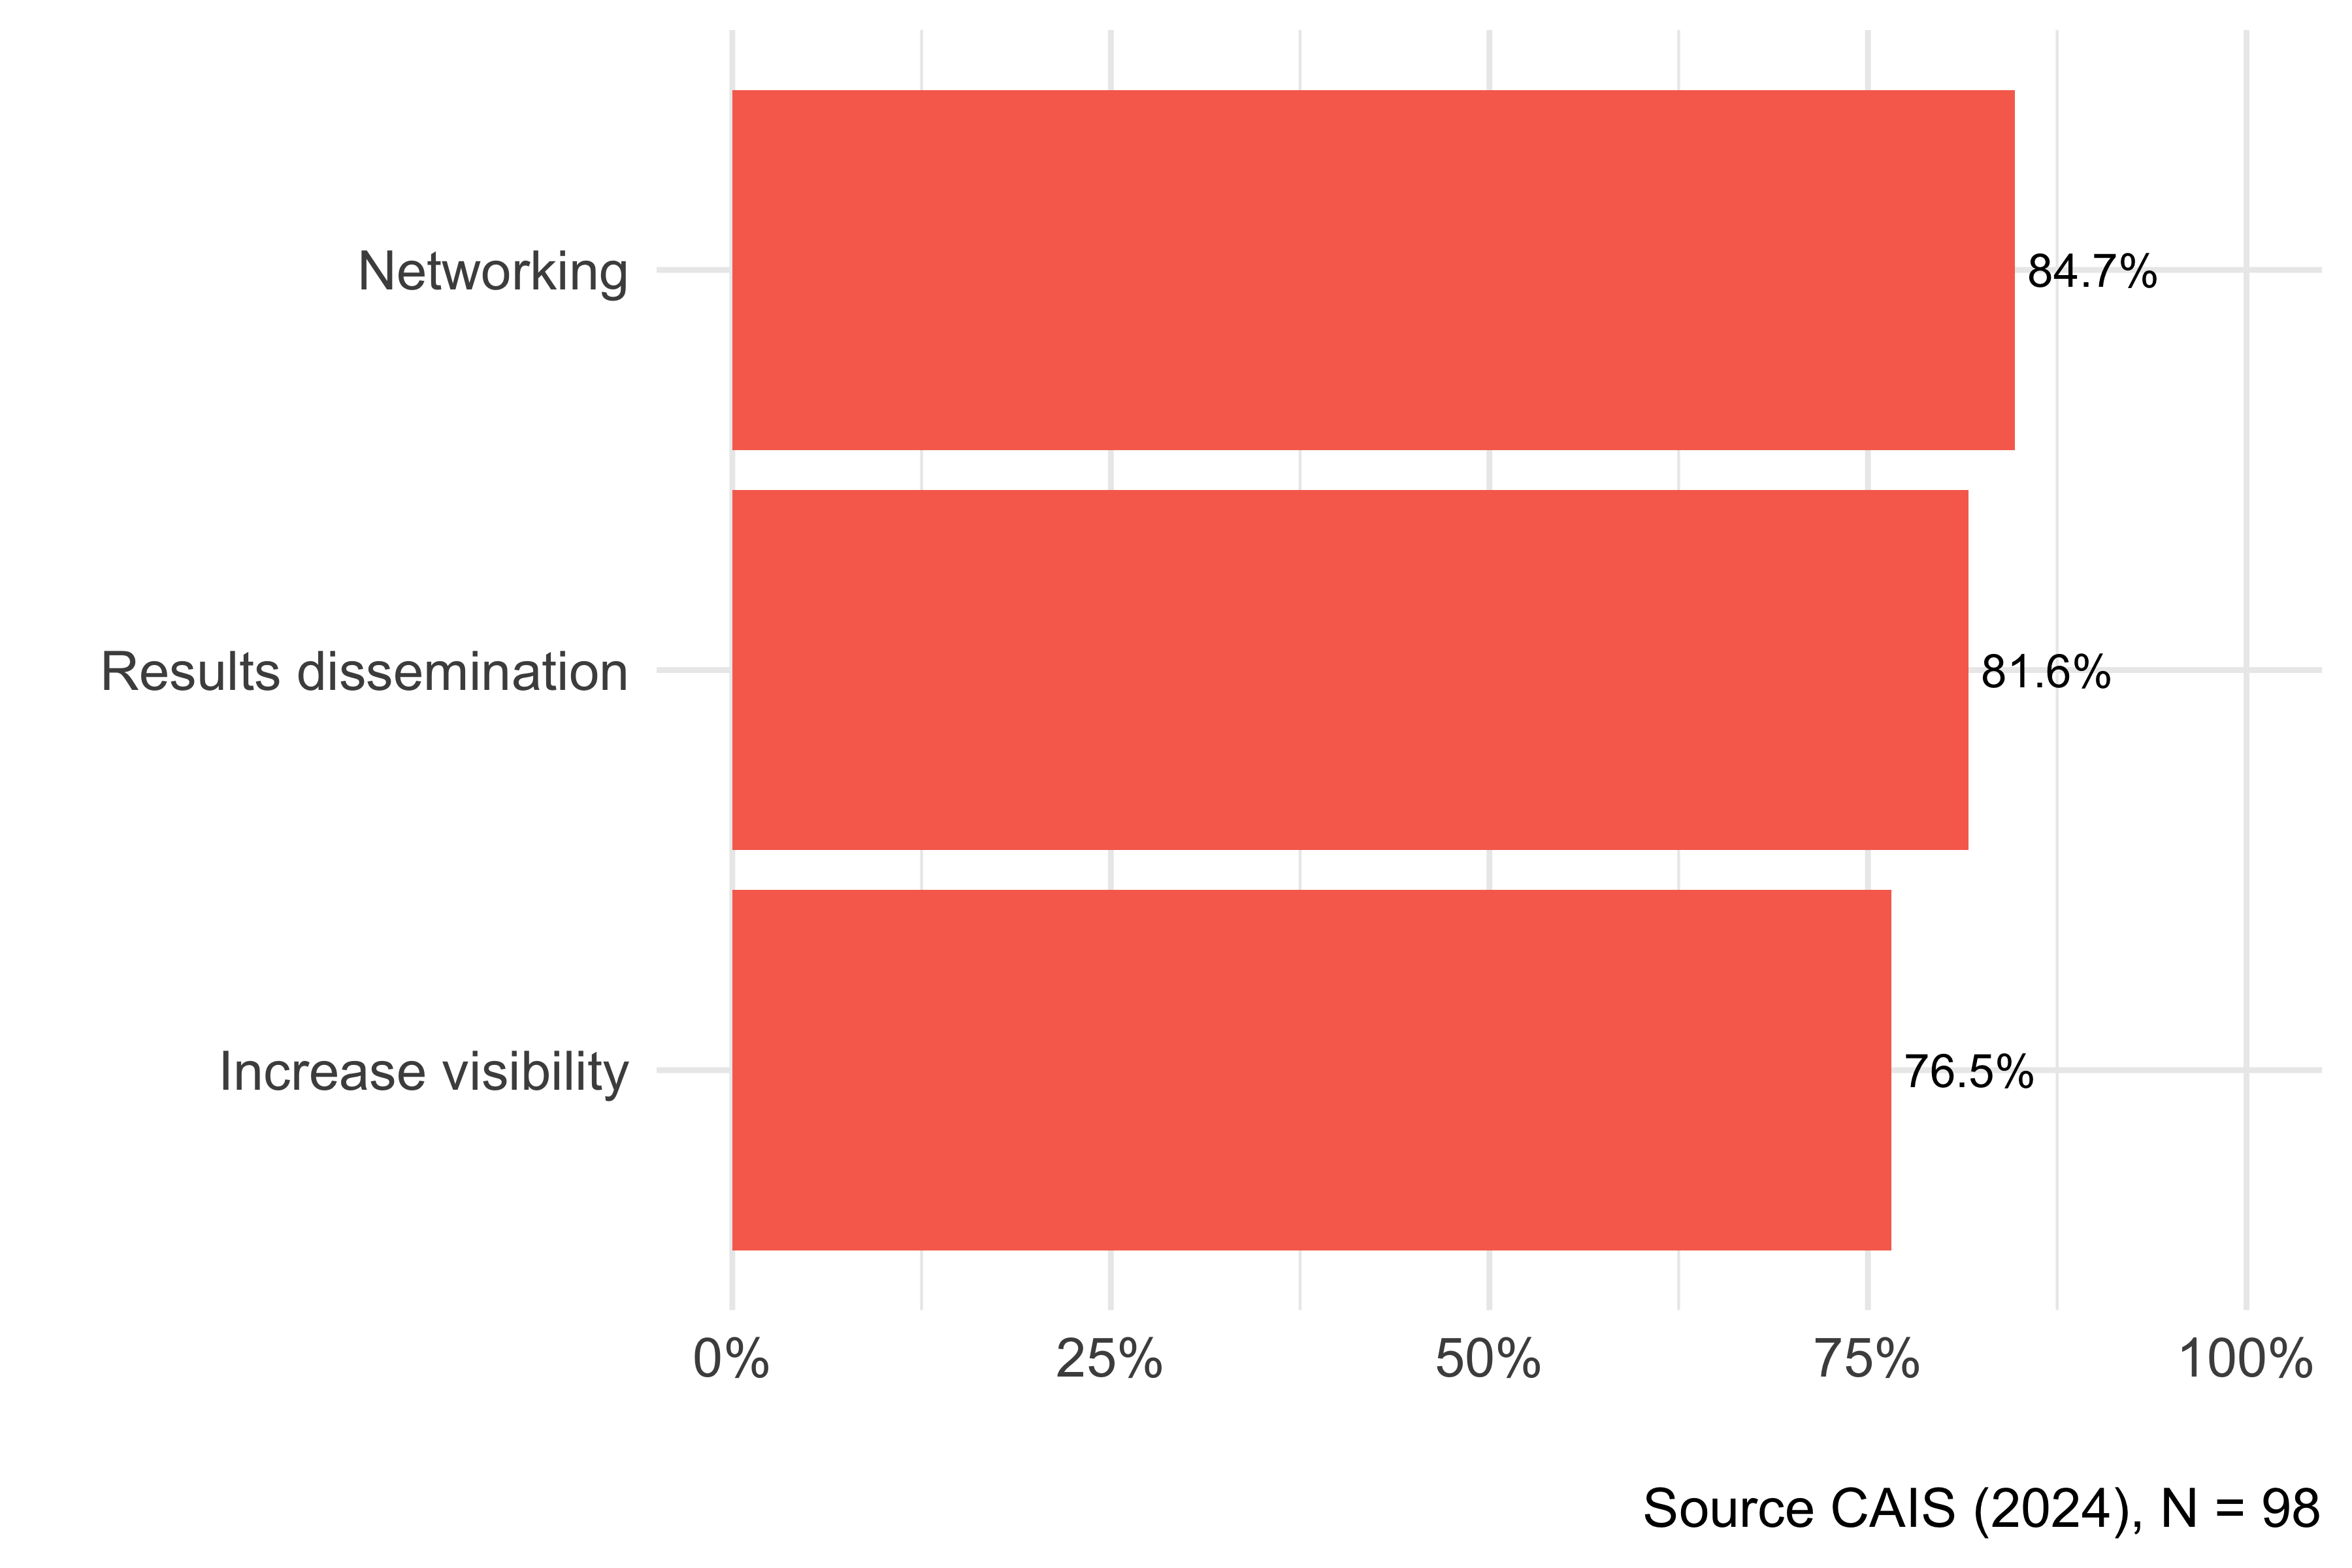
\includegraphics{paper_files/figure-pdf/fig-motivaciones-1.png}

}

\caption{\label{fig-motivaciones}Motivaciones apertura de datos}

\end{figure}

Es interesante constatar que, como se ve en la
Figura~\ref{fig-motivaciones-grid}, difundir resultados es valorado
transversalmente, hay grupos donde la valoración de motivaciones
extrínsecas tienen una mayor preponderancia. Particularmente, el generar
redes y aumentar la visibilidad son incentivos más valorados por mujeres
(Figura~\ref{fig-motivaciones-grid-1}) e investigadores de entre 35 y 49
años (Figura~\ref{fig-motivaciones-grid-2}).

\begin{figure}

\begin{minipage}[t]{\linewidth}

{\centering 

\raisebox{-\height}{

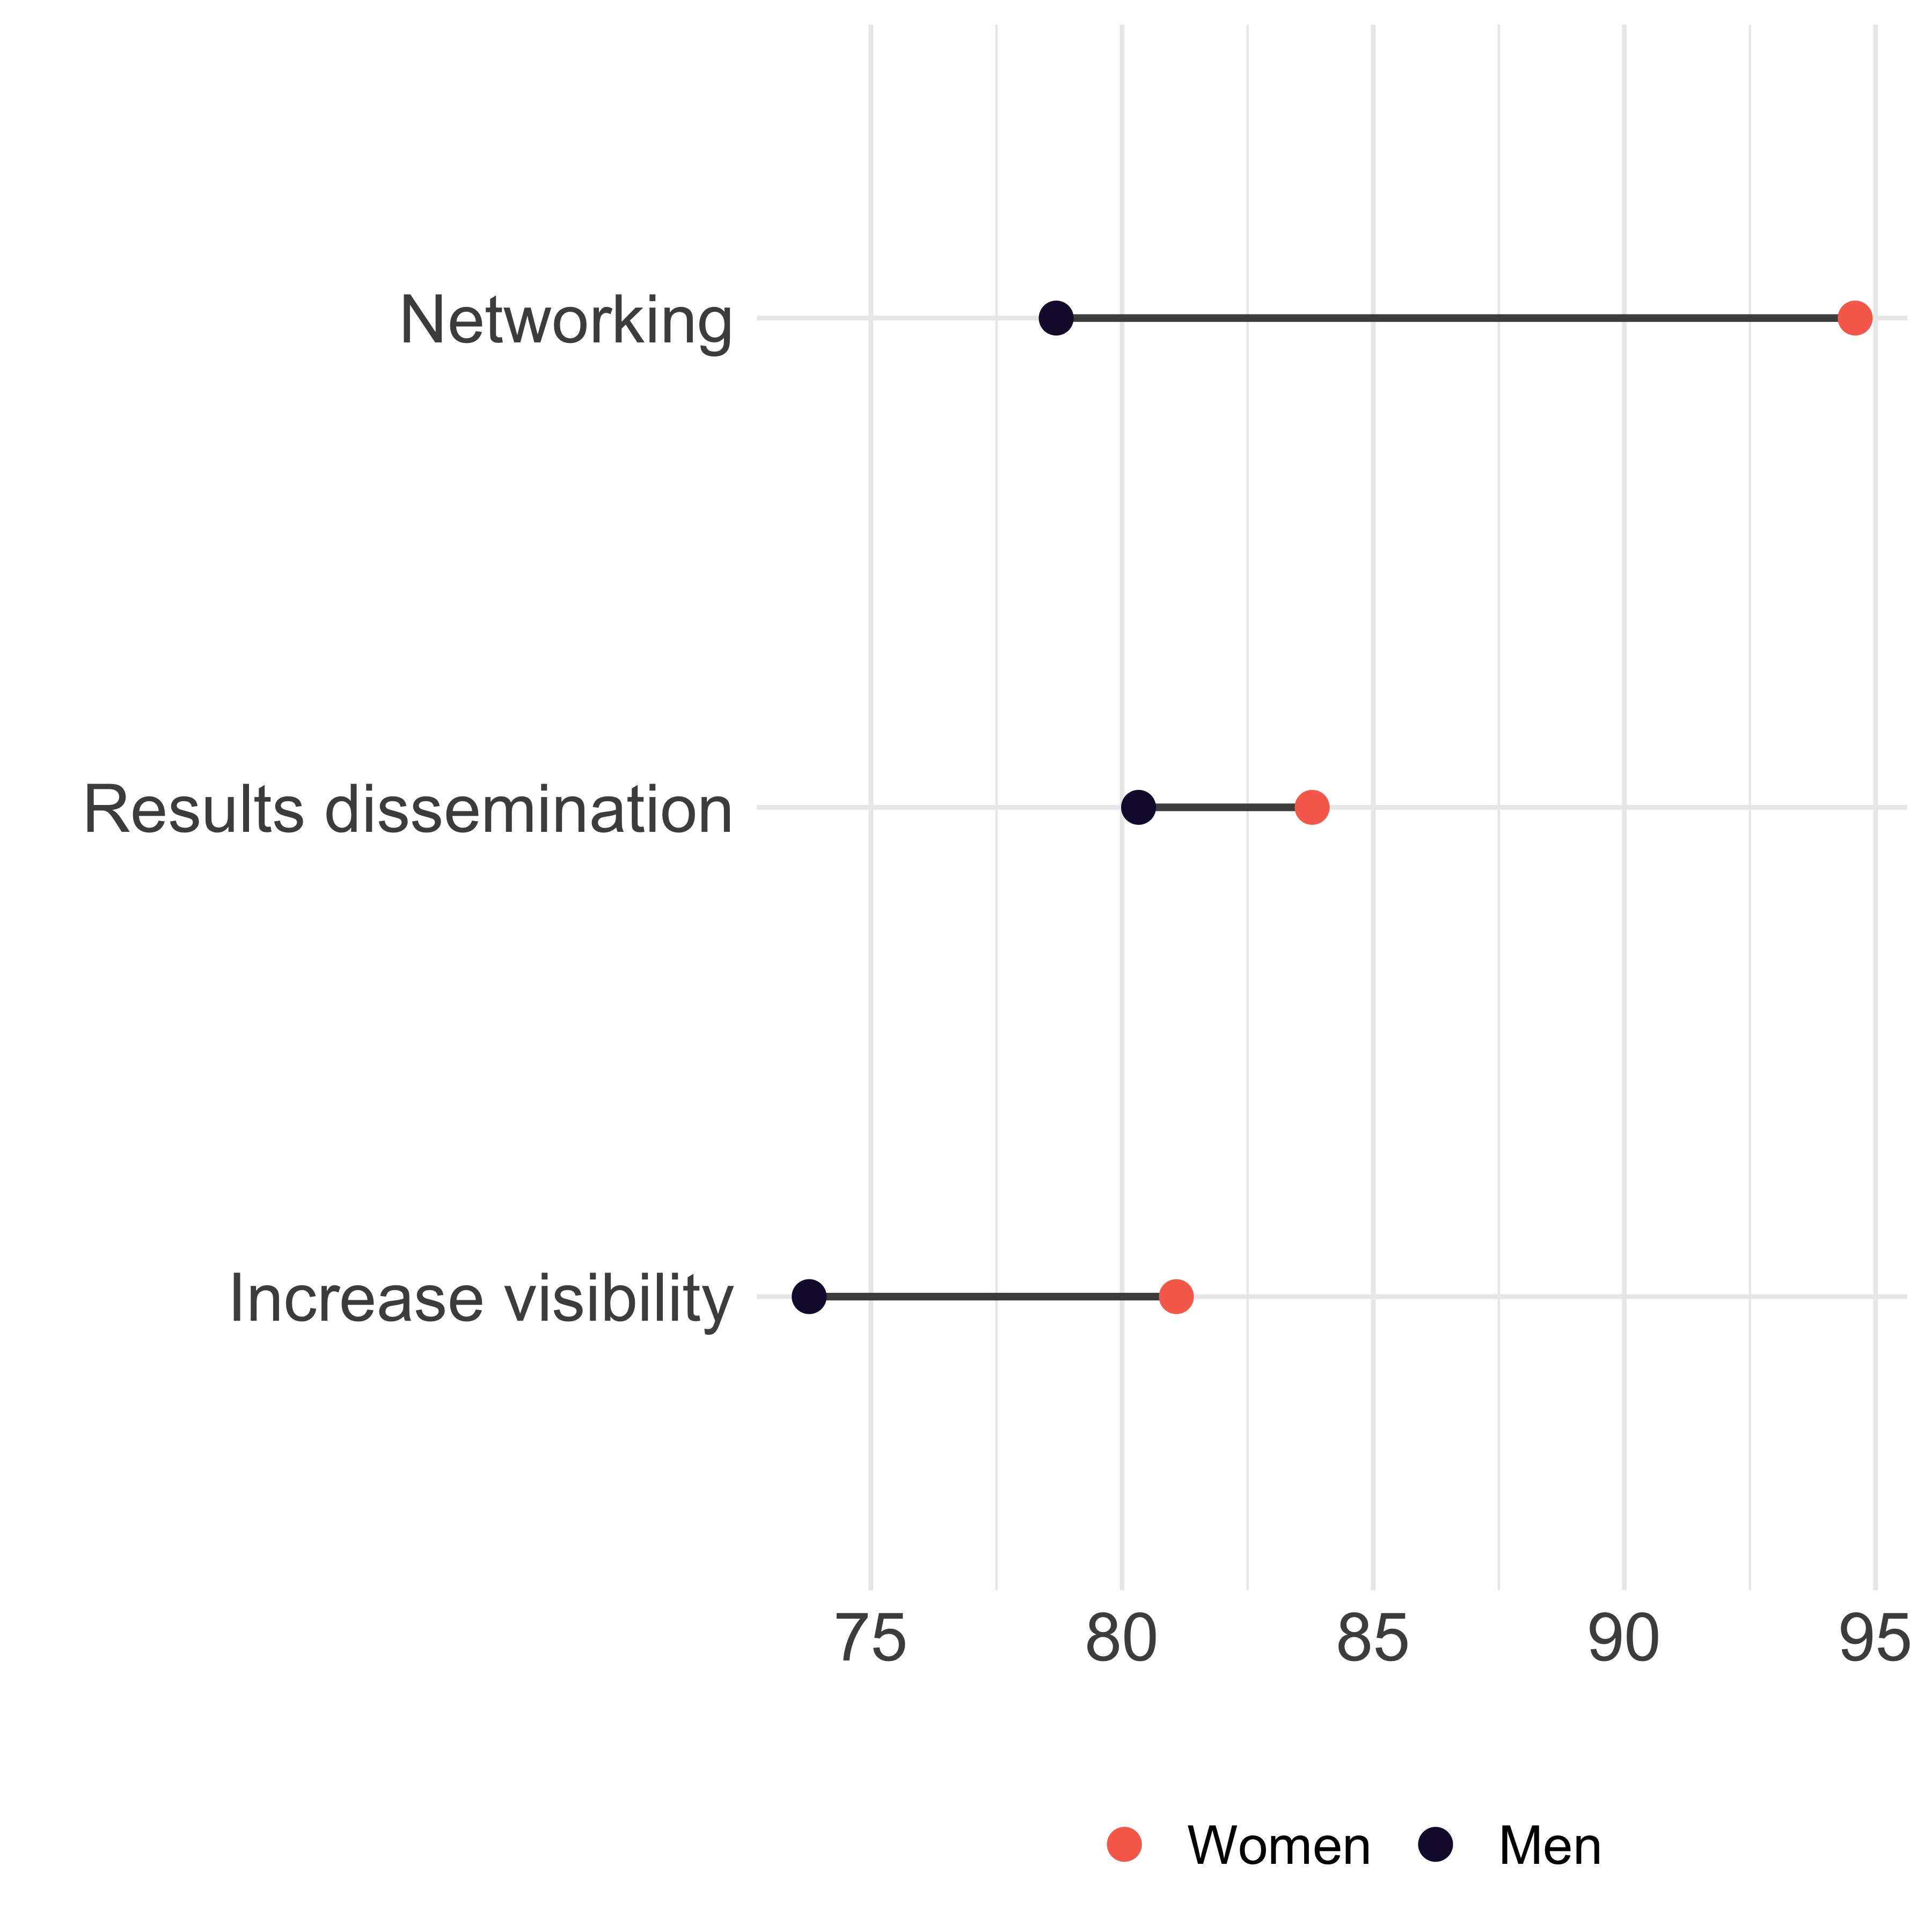
\includegraphics{paper_files/figure-pdf/fig-motivaciones-grid-1.png}

}

}

\subcaption{\label{fig-motivaciones-grid-1}Por sexo}
\end{minipage}%
\newline
\begin{minipage}[t]{\linewidth}

{\centering 

\raisebox{-\height}{

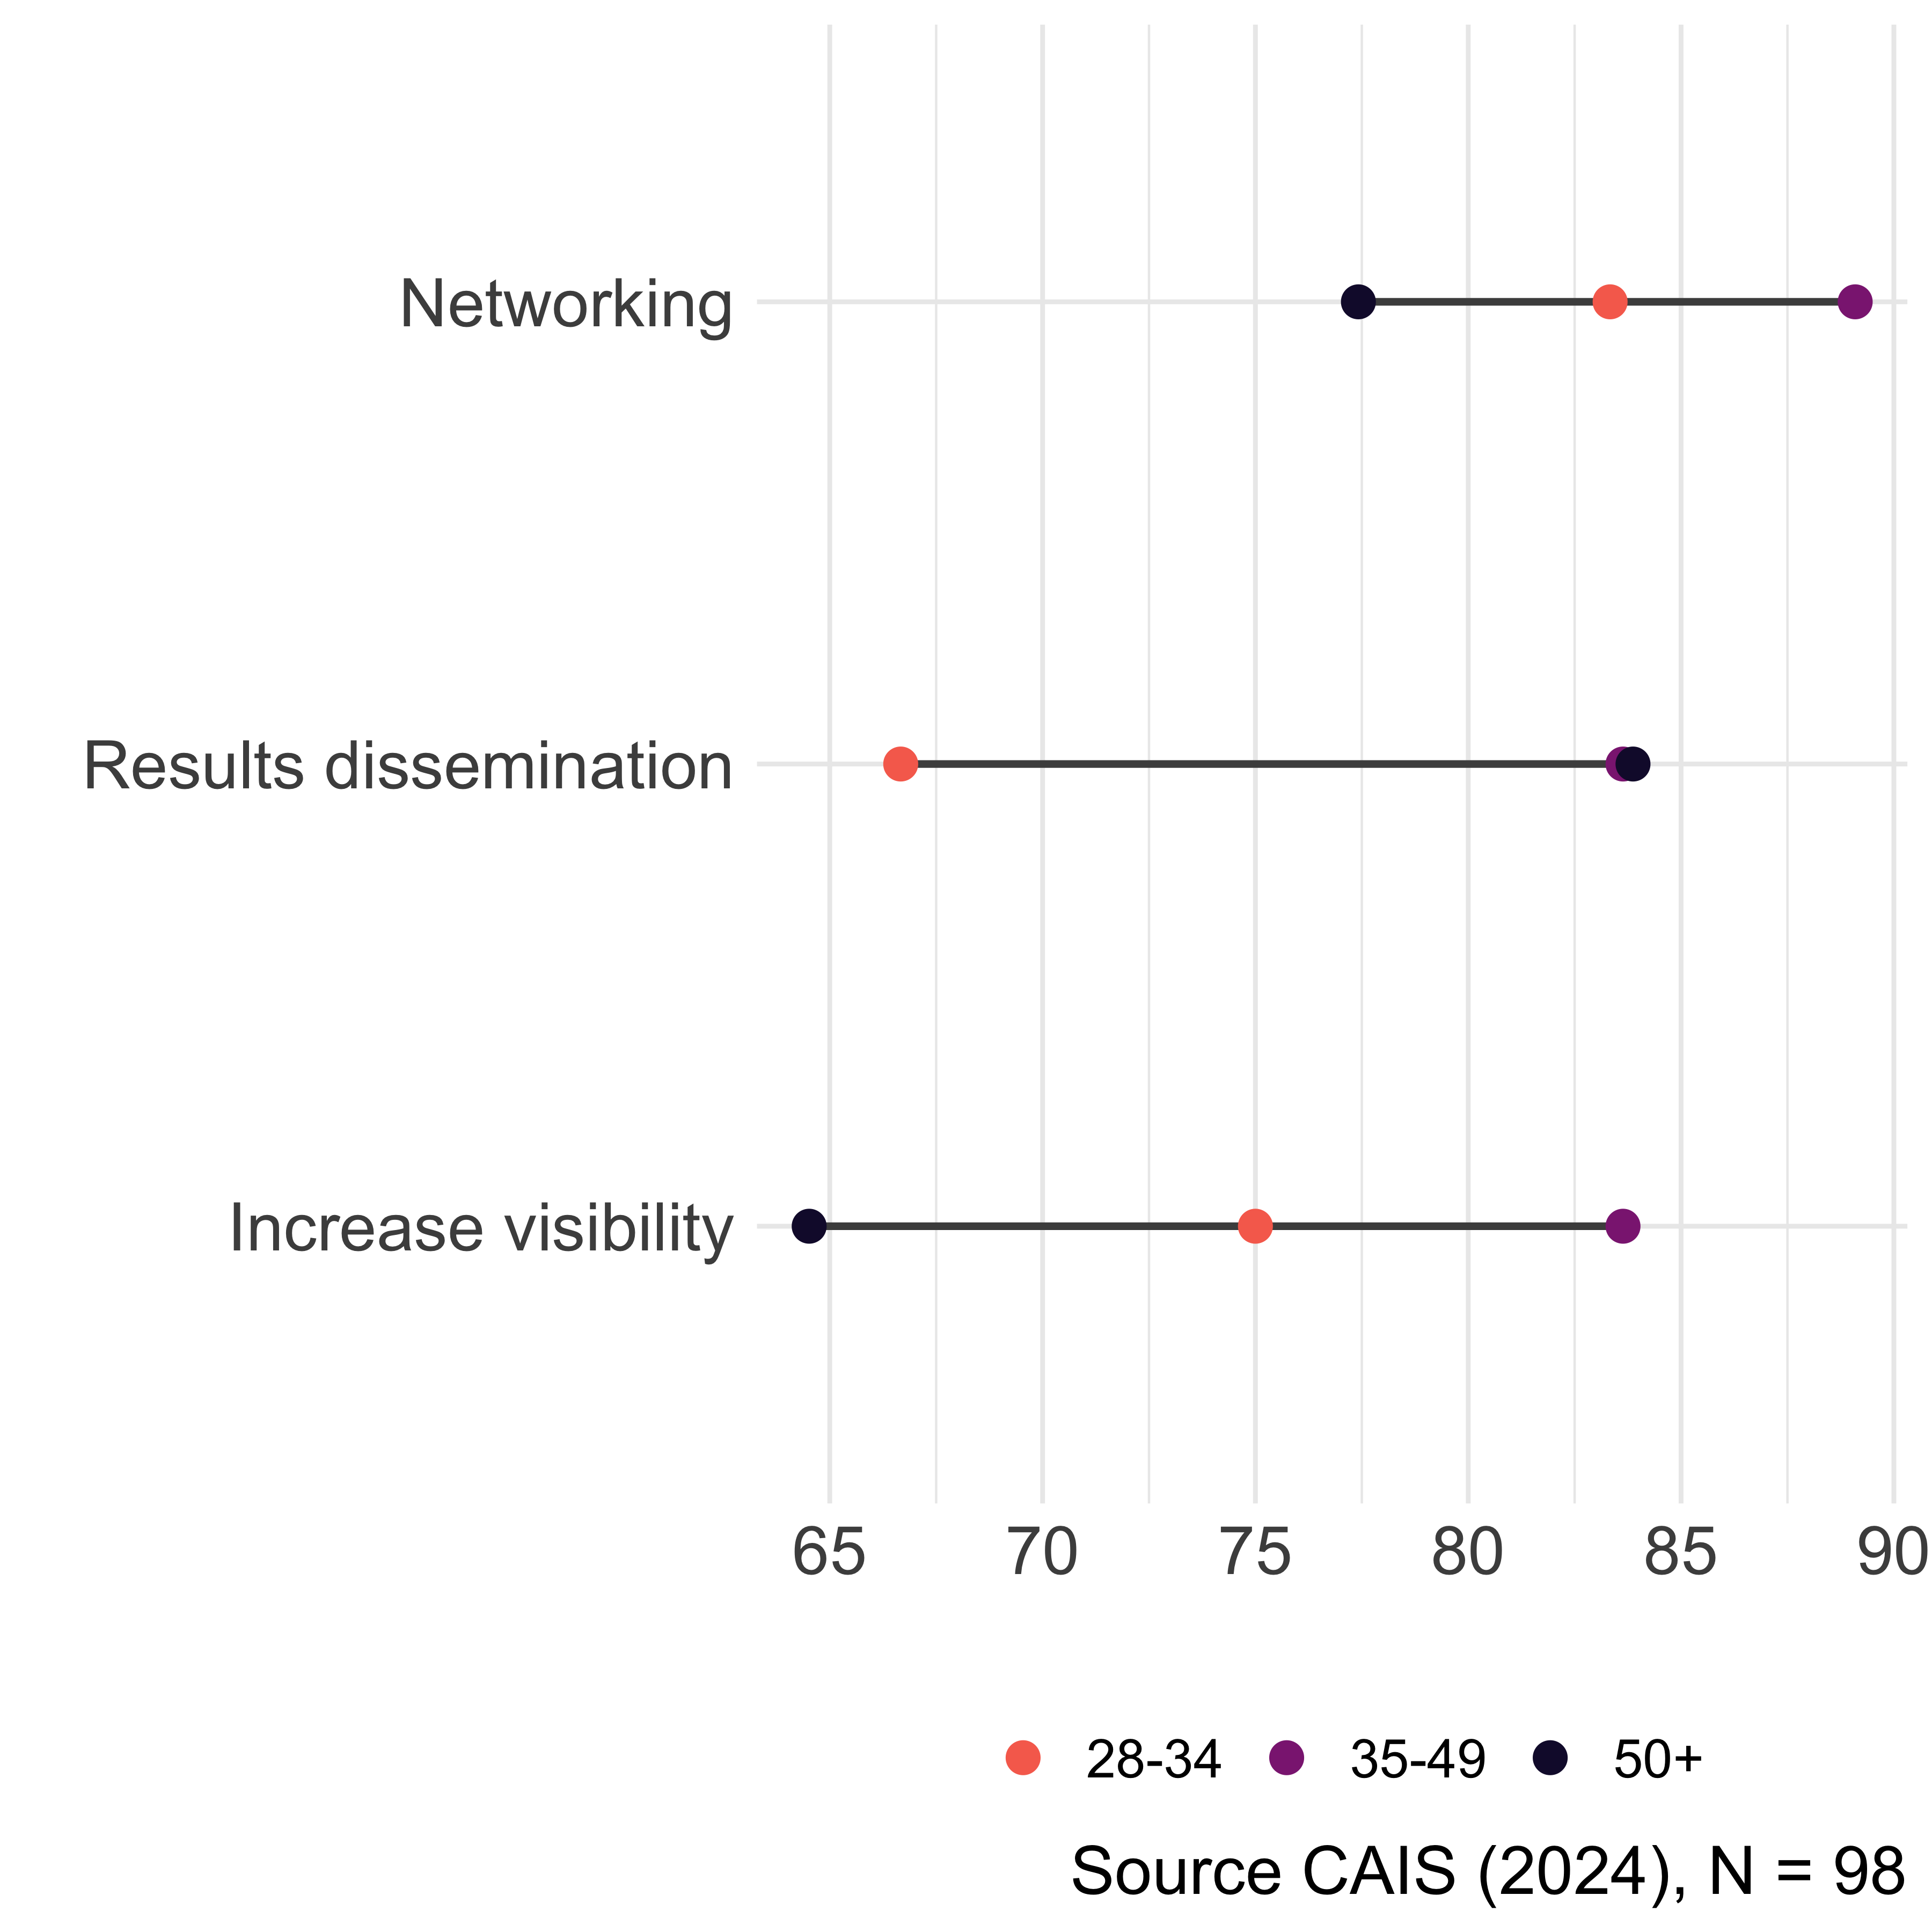
\includegraphics{paper_files/figure-pdf/fig-motivaciones-grid-2.png}

}

}

\subcaption{\label{fig-motivaciones-grid-2}Por edad}
\end{minipage}%

\caption{\label{fig-motivaciones-grid}Motivaciones apertura de datos}

\end{figure}

\textbf{Valoraciones}

\begin{enumerate}
\def\labelenumi{\alph{enumi})}
\tightlist
\item
  Valoraciones sobre medidas de Ciencia Abierta
\end{enumerate}

En general, se valora positivamente la posibilidad de adoptar medidas de
Ciencia Abierta en las Ciencias Sociales, como se puede observar en
Figura~\ref{fig-val} . El acceso abierto (92\%), la replicación de
hallazgos (67\%), el reporte de resultados no estadísticamente
significativos (76\%), y la disponibilización en línea de datos y
materiales de análisis (72\%), todas muestran un alto nivel de
aceptación entre los encuestados. La única excepción es el pre-registro
de hipótesis, que solo tiene un 42\% de evaluación positiva. Esto se
explica por un mayor nivel de desconocimiento (17\% dice no conocer la
medida), además de las reticencias ya observadas en las entrevistas del
estudio cualitativo.

\begin{figure}

{\centering 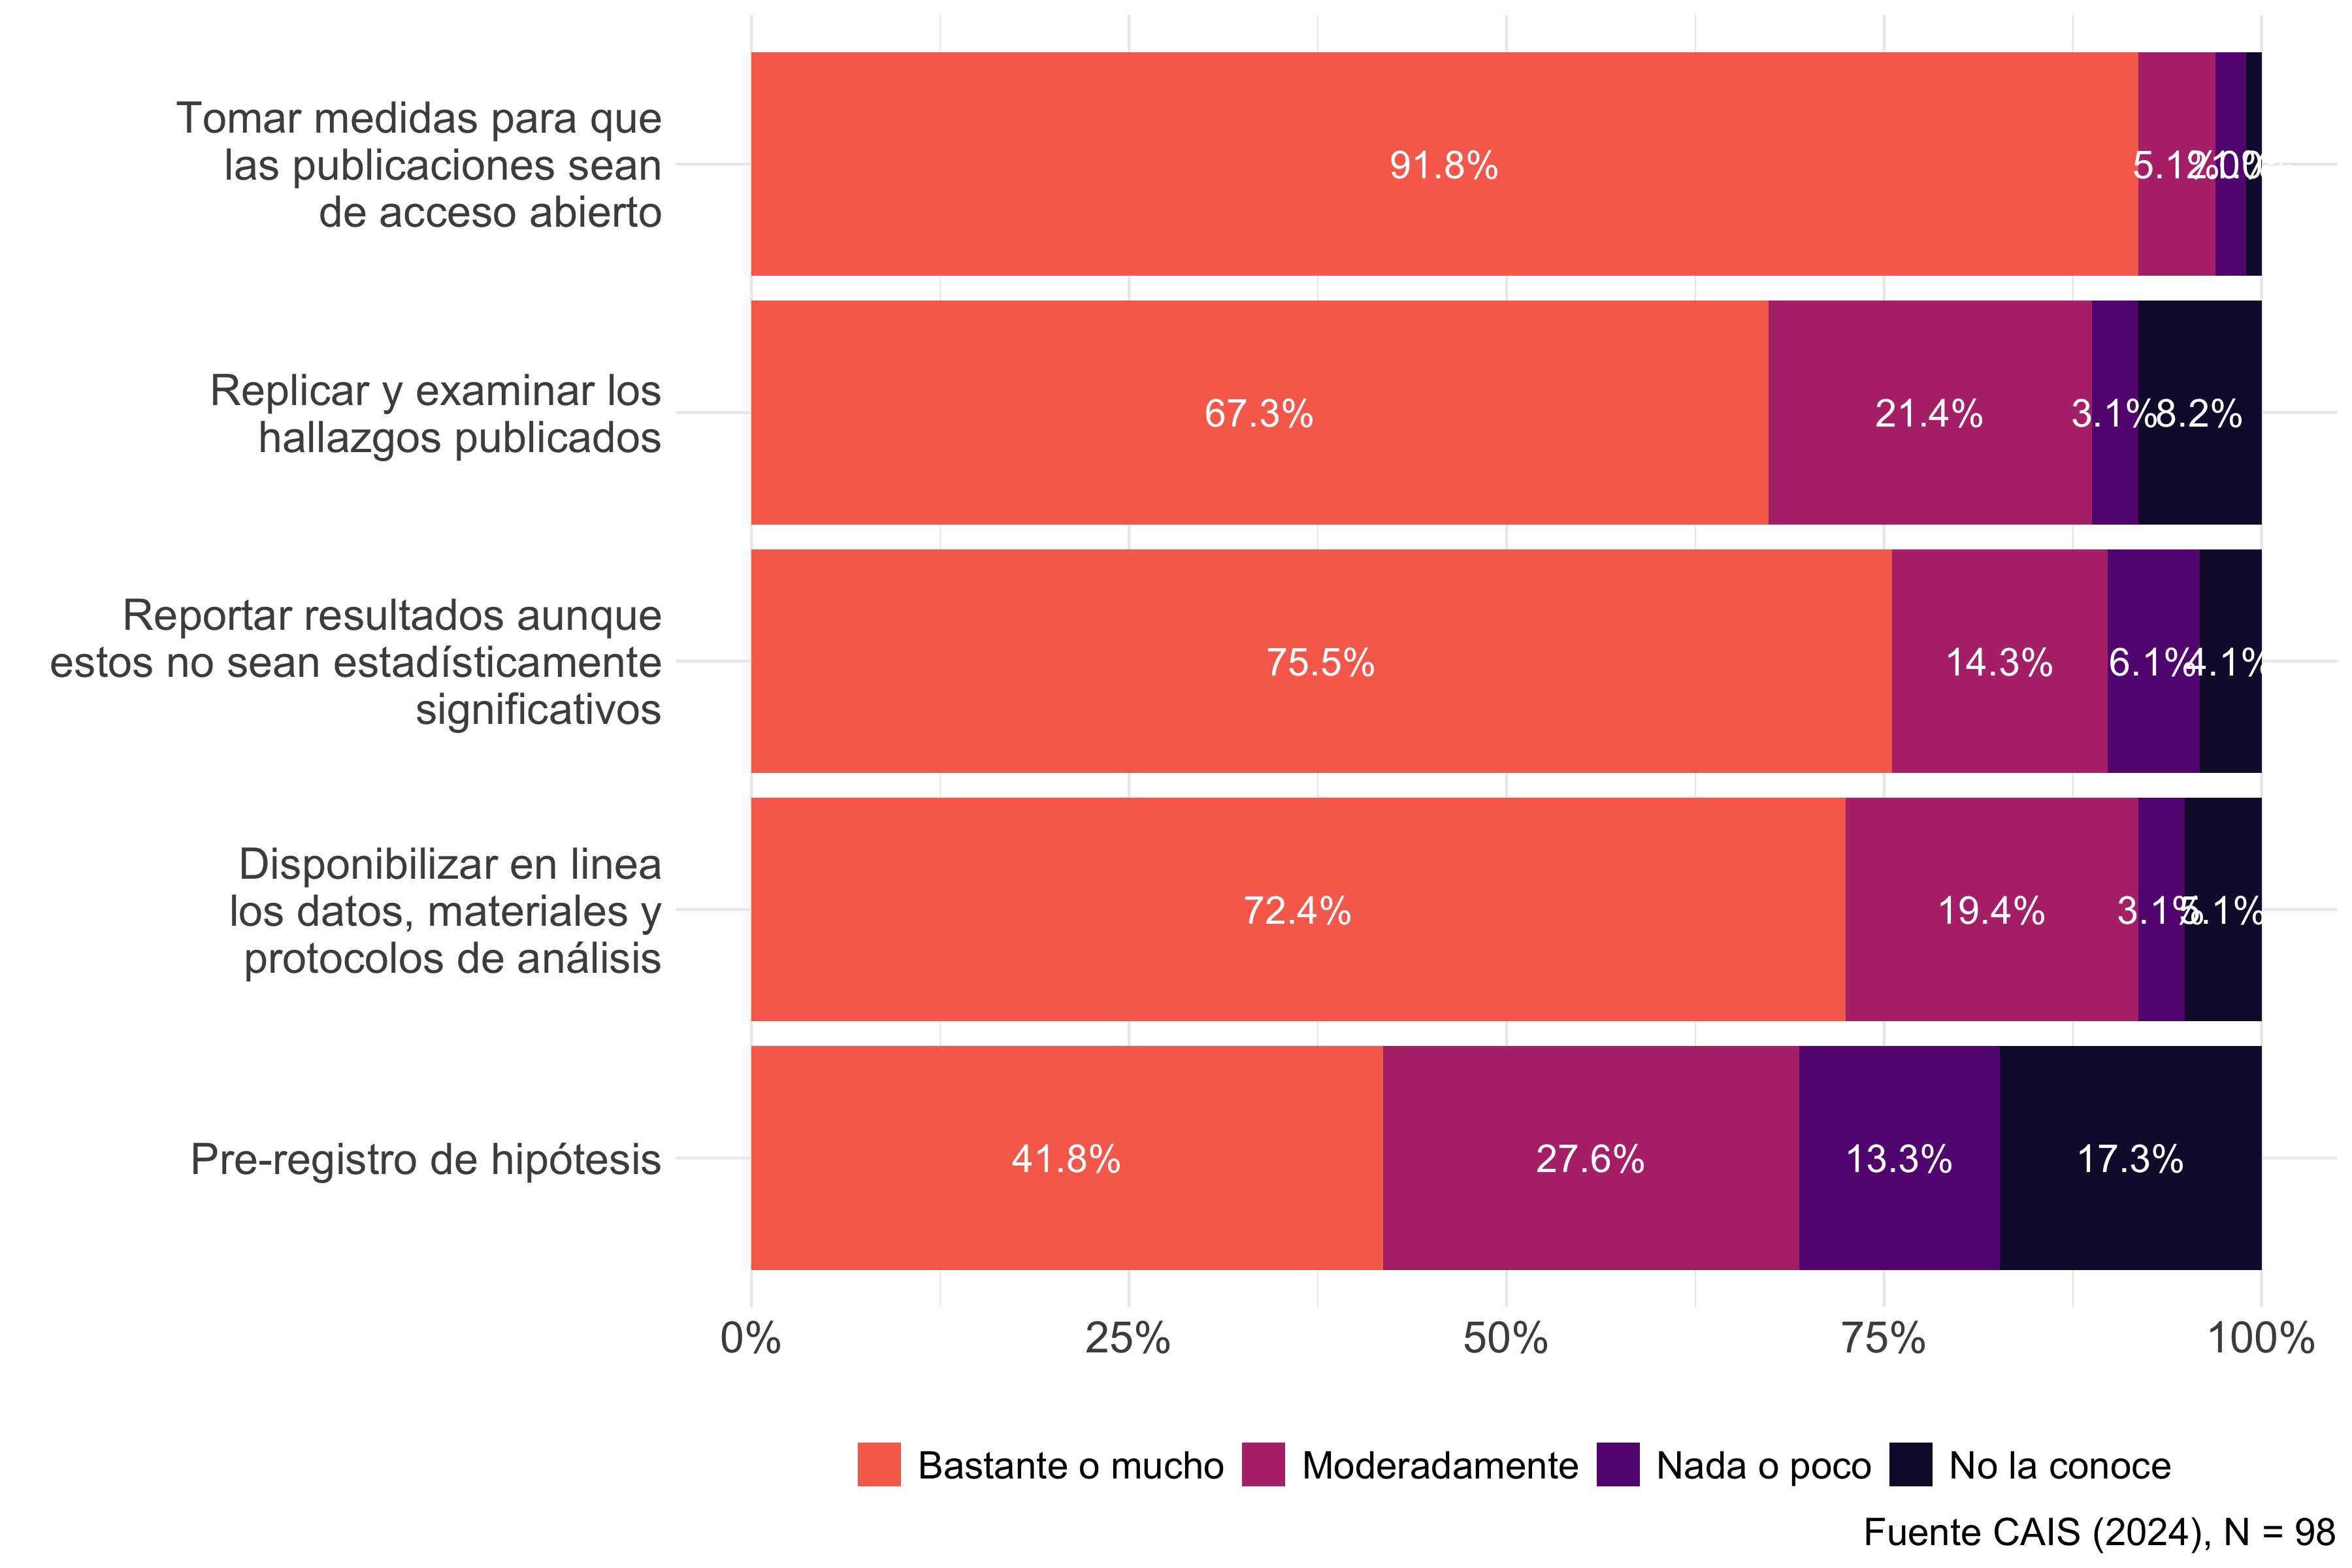
\includegraphics{paper_files/figure-pdf/fig-val-1.png}

}

\caption{\label{fig-val}¿Qué tan necesarias cree que son las siguientes
medidas impulsadas por la CA para la investigación en Ciencias
Sociales?}

\end{figure}

Salvo por el acceso abierto a publicaciones, que es valorada
transversalmente por todos los grupos, estas medidas son apoyadas en
mayor medida por investigadoras mujeres y por investigadores con enfoque
cuantitativo, como se puede apreciar en la Figura~\ref{fig-vca-grid}.

\begin{figure}

\begin{minipage}[t]{\linewidth}

{\centering 

\raisebox{-\height}{

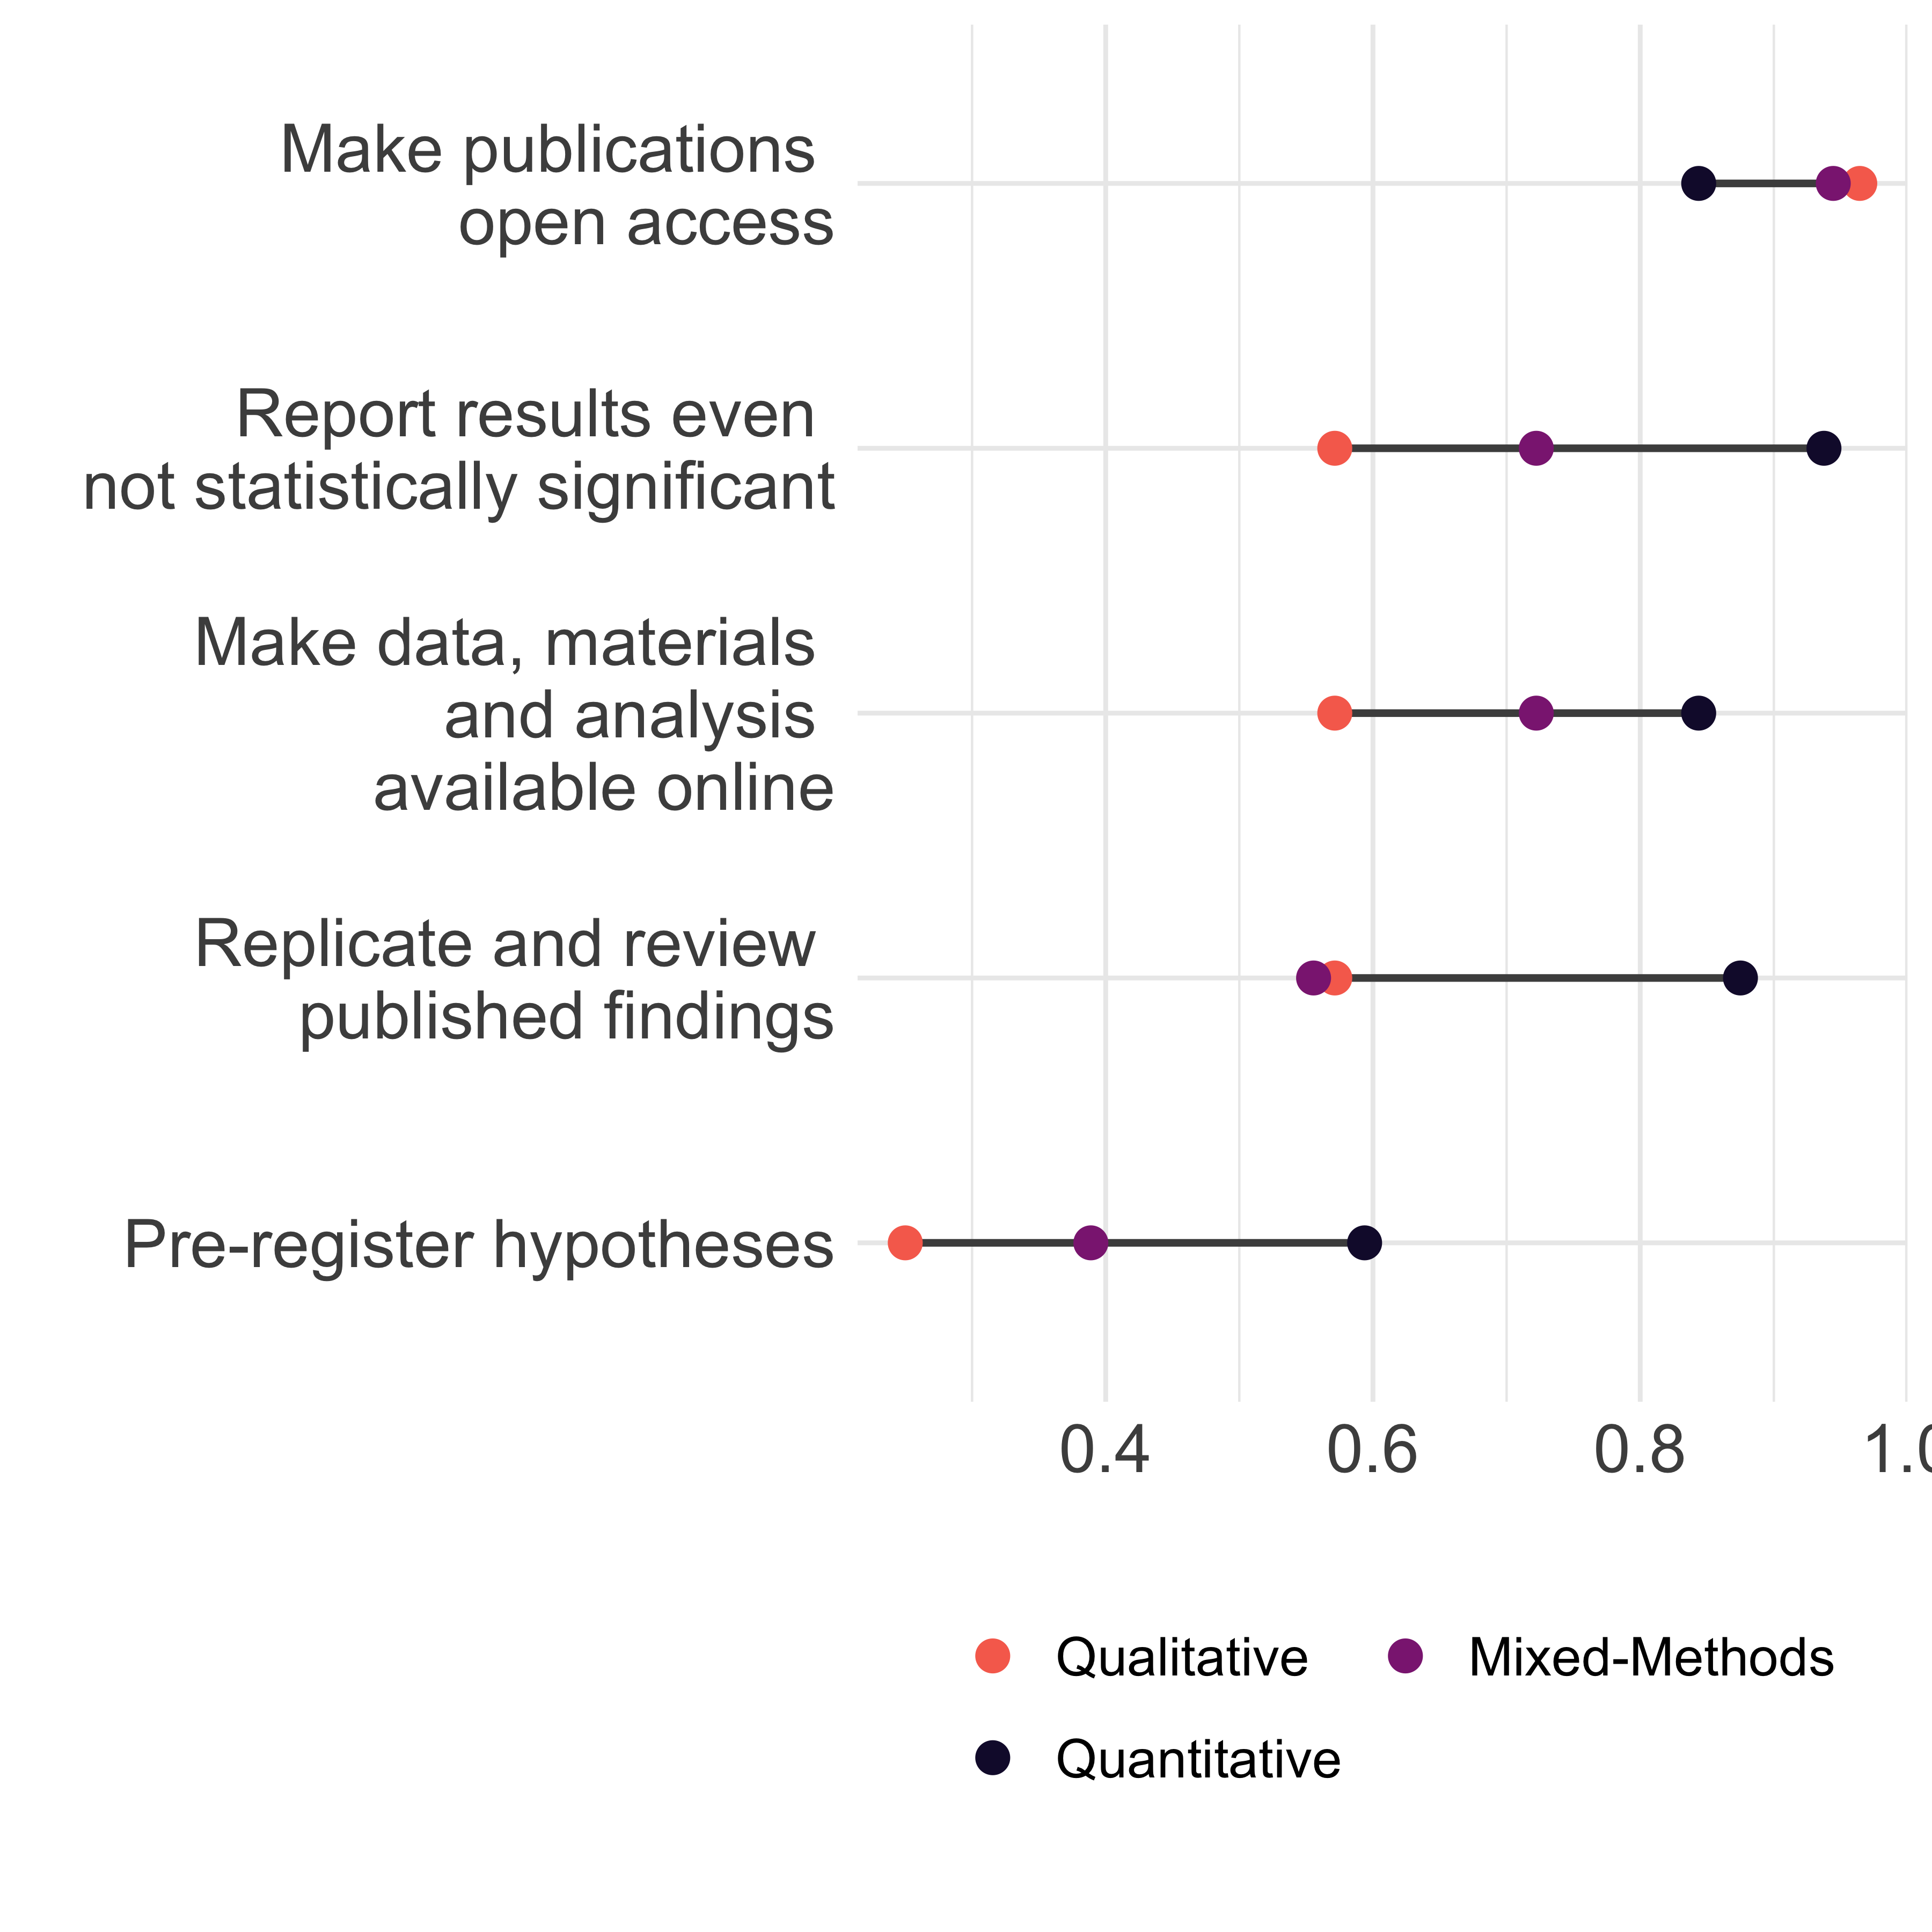
\includegraphics{paper_files/figure-pdf/fig-vca-grid-1.png}

}

}

\subcaption{\label{fig-vca-grid-1}Por sexo}
\end{minipage}%
\newline
\begin{minipage}[t]{\linewidth}

{\centering 

\raisebox{-\height}{

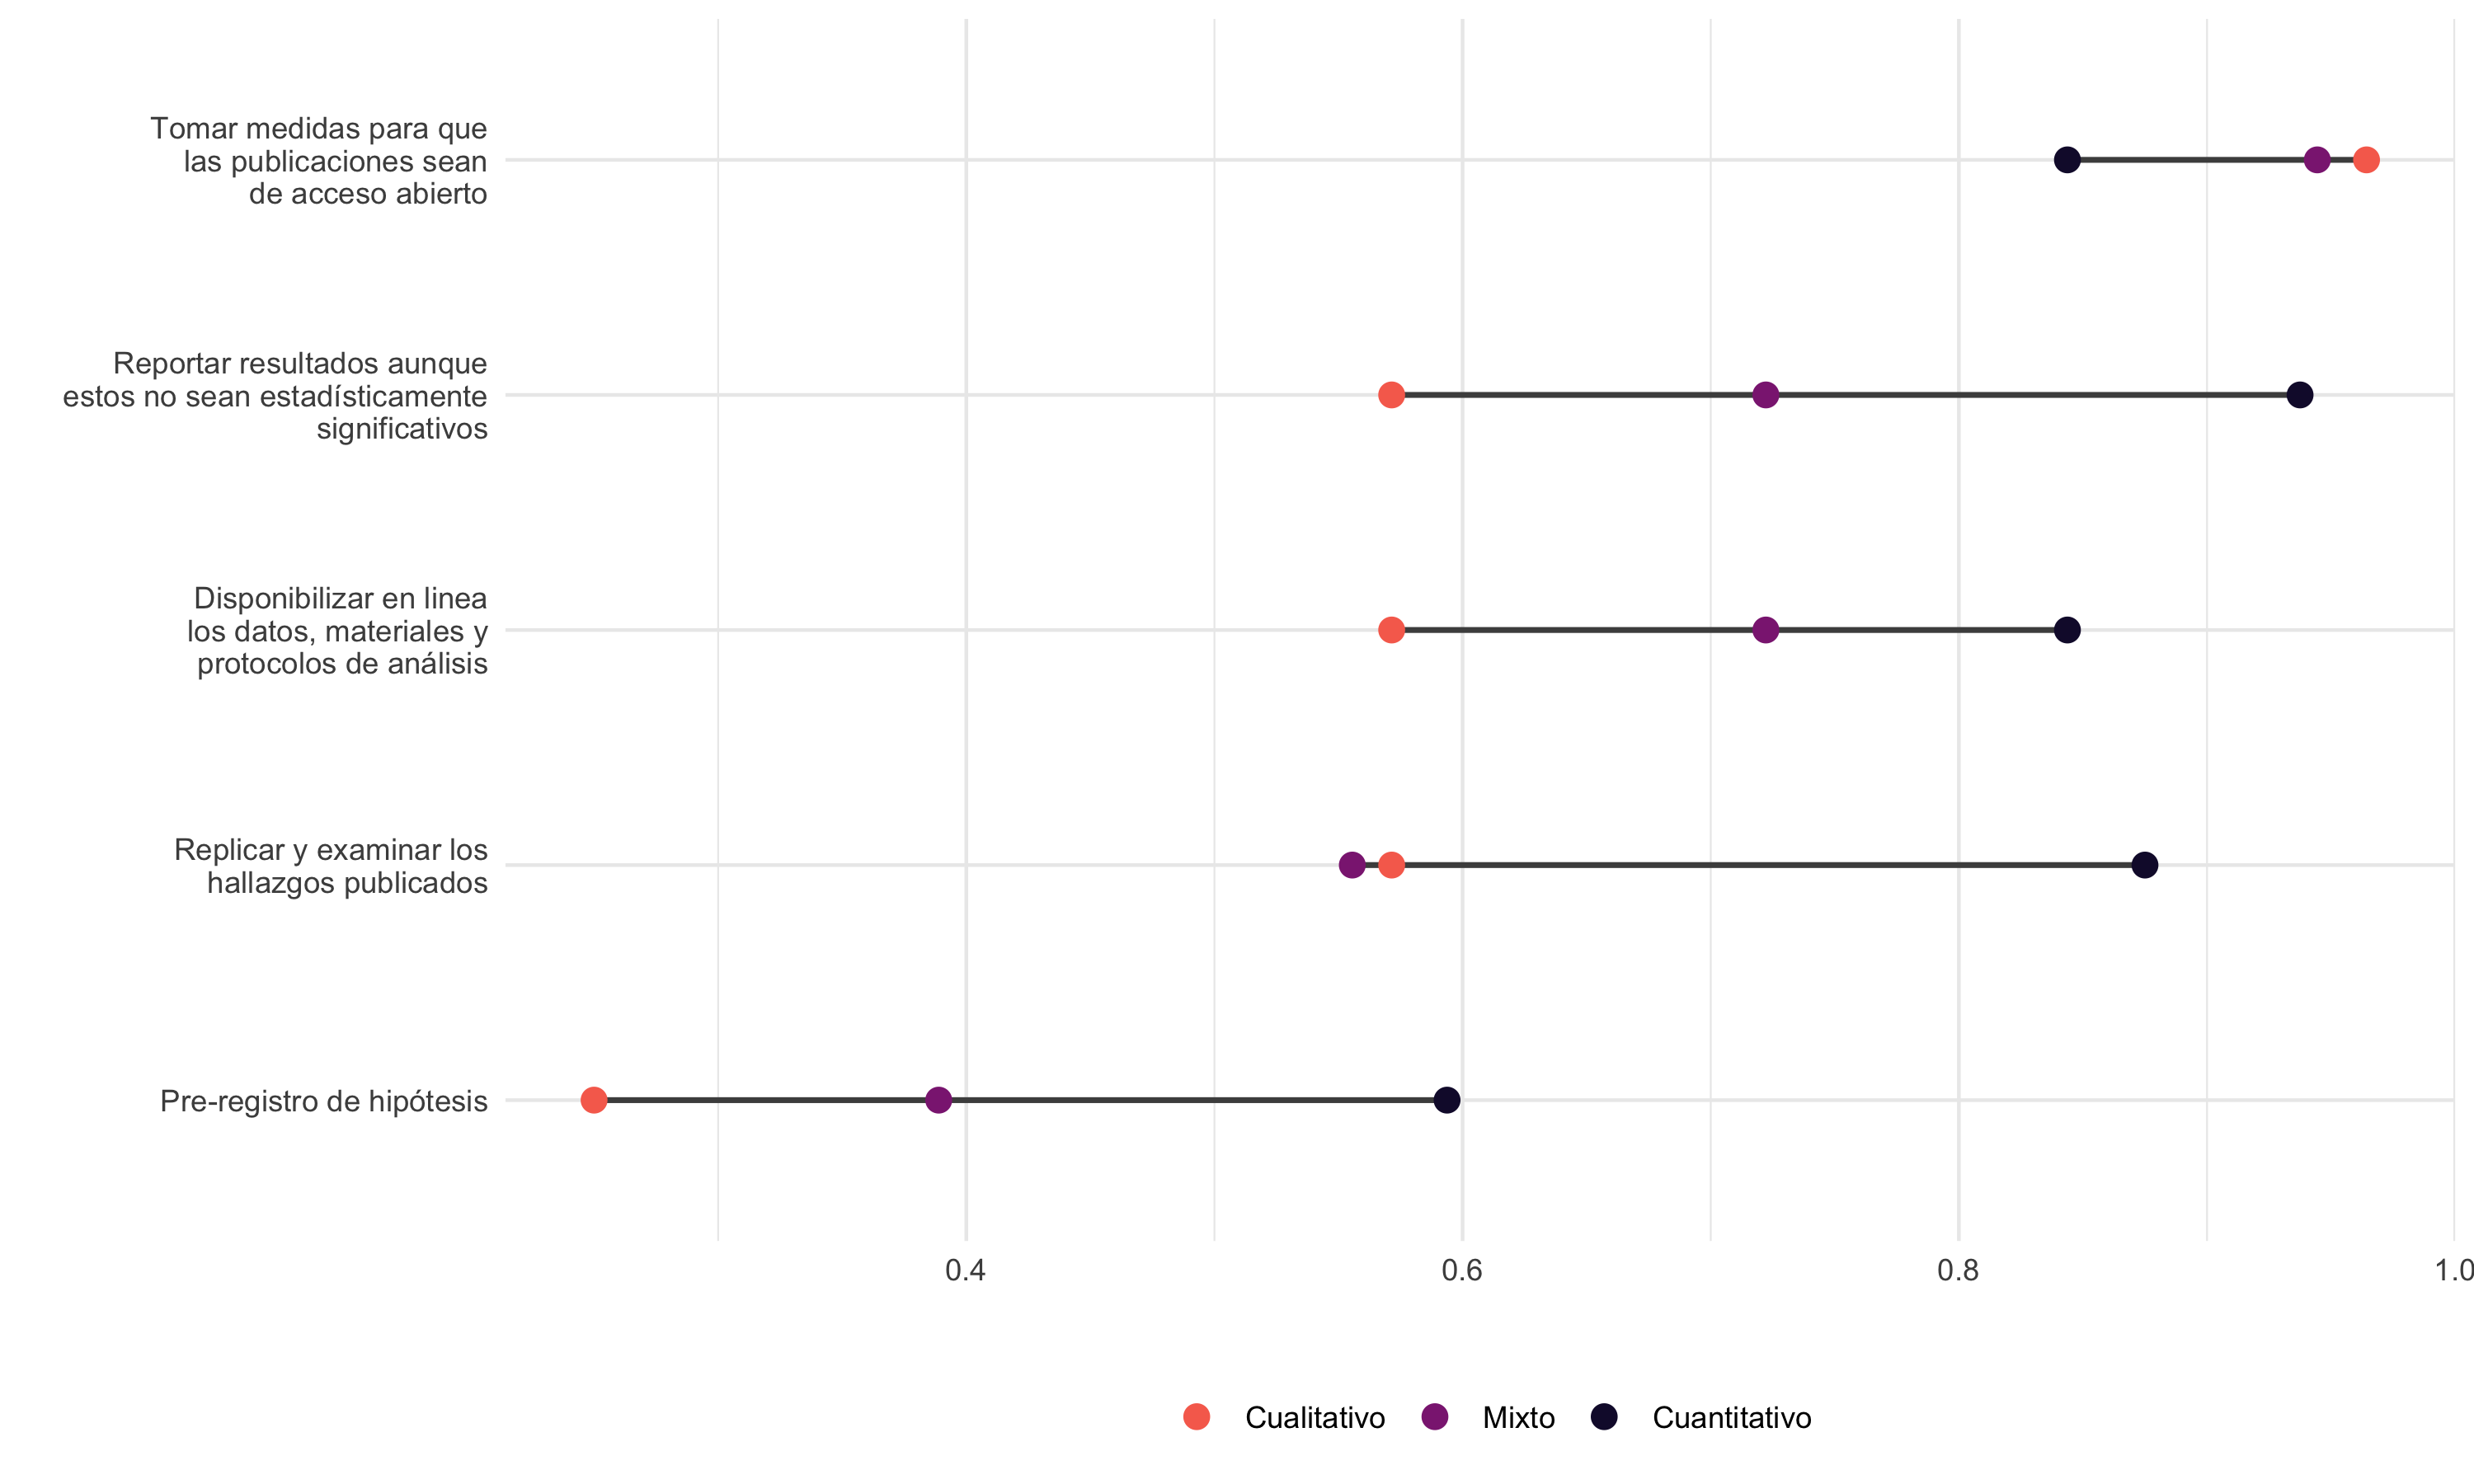
\includegraphics{paper_files/figure-pdf/fig-vca-grid-2.png}

}

}

\subcaption{\label{fig-vca-grid-2}Por enfoque}
\end{minipage}%

\caption{\label{fig-vca-grid}¿Qué tan necesarias cree que son las
siguientes medidas impulsadas por la CA para la investigación en
Ciencias Sociales?, por sexo y enfoque de investigación}

\end{figure}

\begin{enumerate}
\def\labelenumi{\alph{enumi})}
\setcounter{enumi}{1}
\tightlist
\item
  Valoraciones sobre la Crisis de Reproducibilidad
\end{enumerate}

Como se evidencia en la Figura~\ref{fig-dona}, el 39\% de los
encuestados cree que hay una crisis importante de reproducibilidad,
mientras que el 40\% no sabe si la hay.

\begin{figure}

{\centering 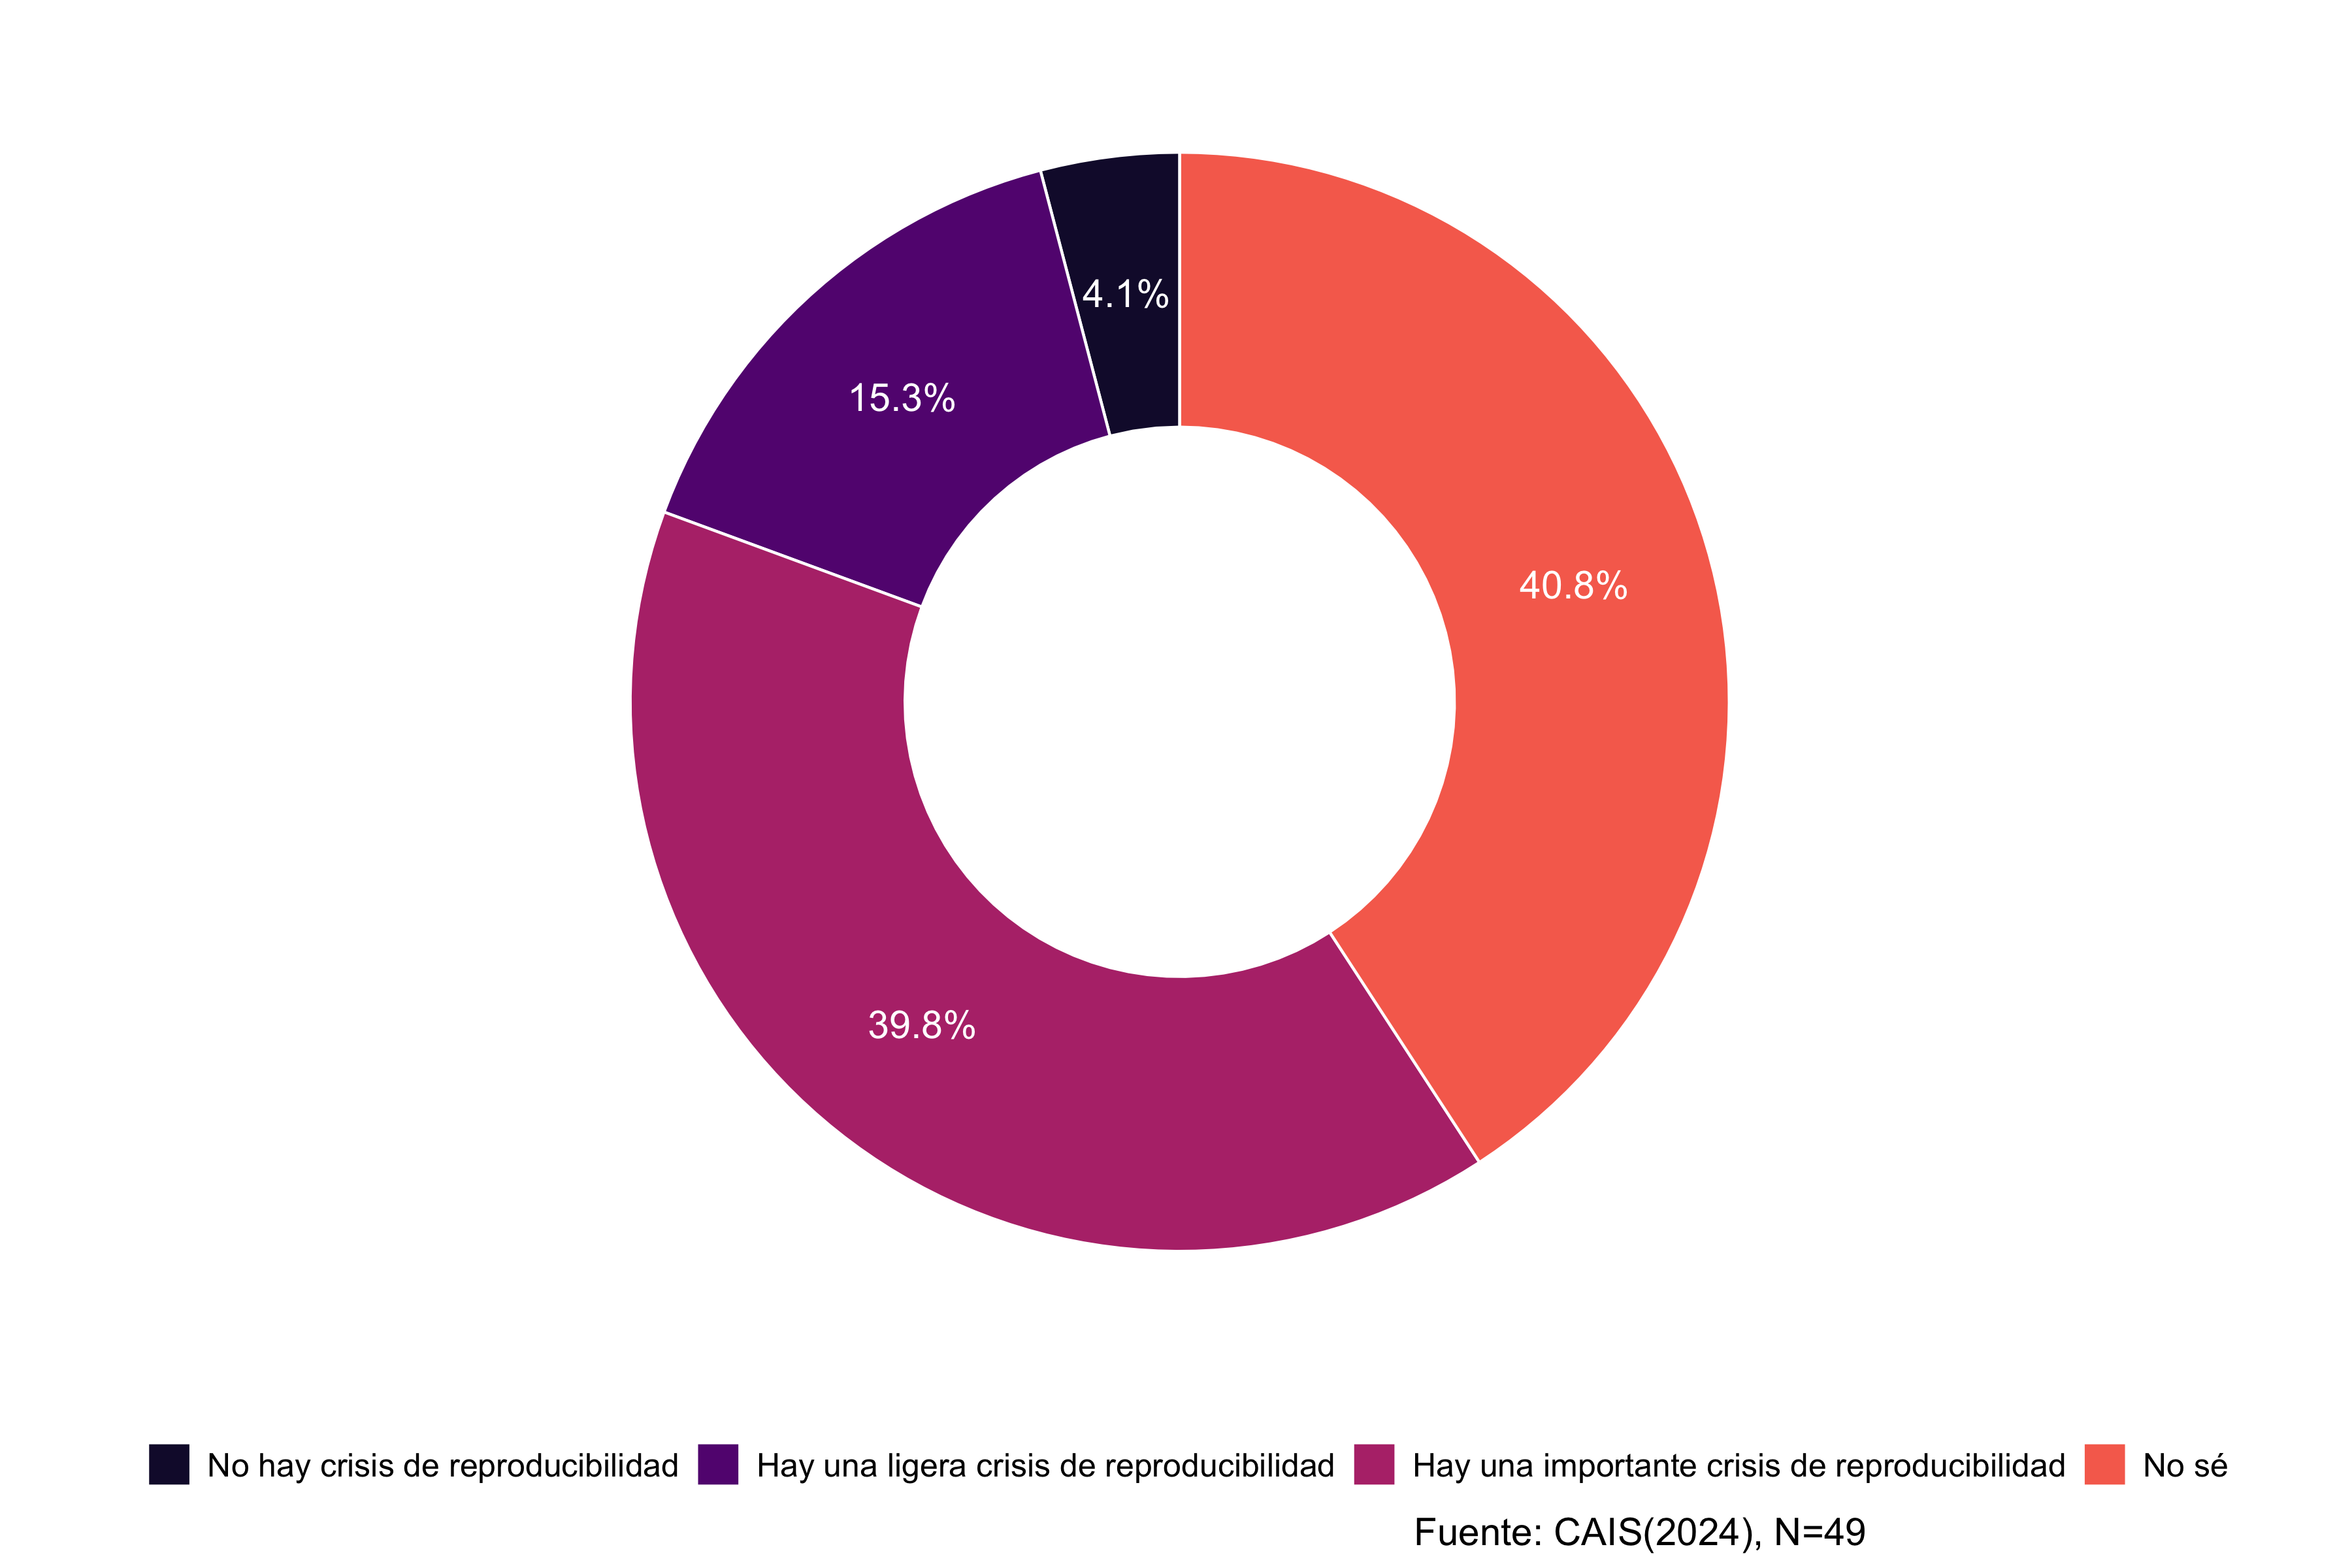
\includegraphics{paper_files/figure-pdf/fig-dona-1.png}

}

\caption{\label{fig-dona}¿Con cuál de las siguientes afirmaciones
respecto a la crisis de reproducibilidad está de acuerdo?}

\end{figure}

Además, se identificaron diferencias respecto al enfoque de
investigación (ver Figura~\ref{fig-dona-grid}). La preocupación es mayor
entre los investigadores cuantitativos, ya que el 70\% cree que la
crisis es importante. Si bien entre los investigadores cualitativos no
se llega a negar la crisis, sí hay un 60\% que desconoce si la hay o no.

\begin{figure}

{\centering 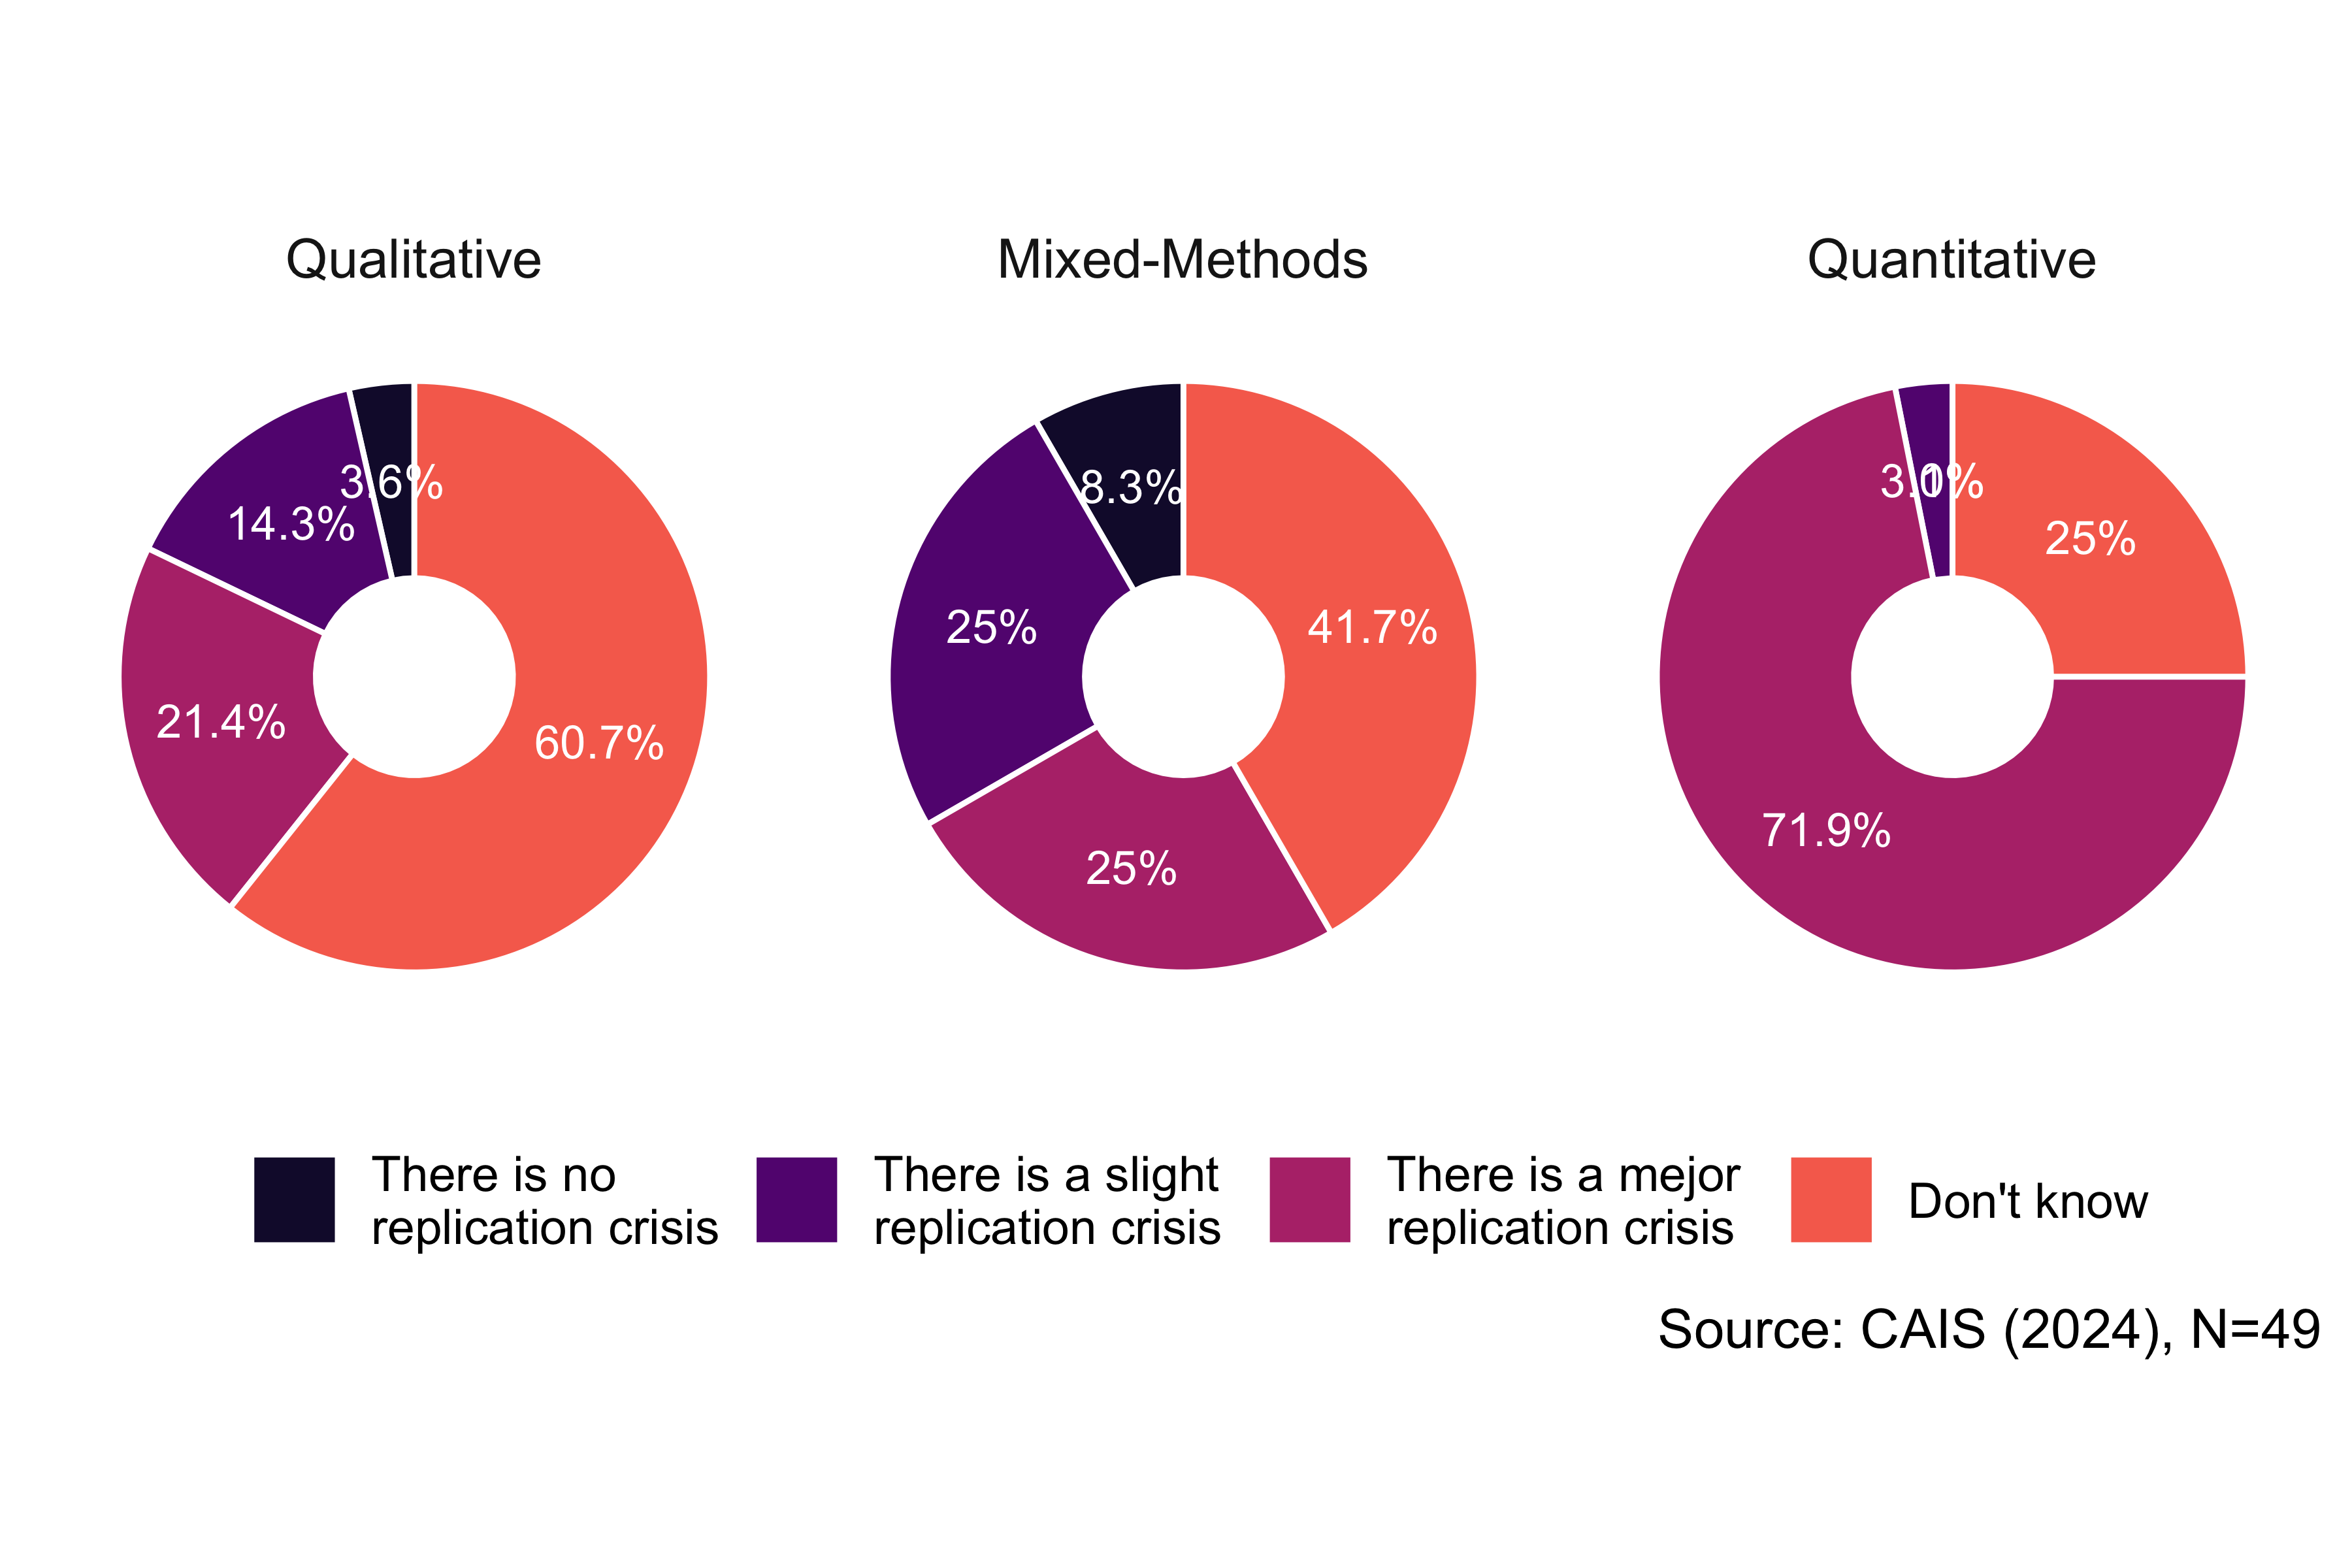
\includegraphics{paper_files/figure-pdf/fig-dona-grid-1.png}

}

\caption{\label{fig-dona-grid}Percepcion sobre la crisis de
reproducibilidad por enfoque.}

\end{figure}

Por otro lado, el 59\% cree que el 30\% o menos de las investigaciones
en ciencias sociales son reproducibles; el 83\% cree que menos de la
mitad de las investigaciones en ciencias sociales son reproducibles,
como se muestra en Tabla~\ref{tbl-tablaacum}.

Investigaciones

\hypertarget{tbl-tablaacum}{}
\begin{longtable}[]{@{}rrr@{}}
\caption{\label{tbl-tablaacum}Percepción de porcentaje de
investigaciones reproducibles en Ciencias Sociales}\tabularnewline
\toprule\noalign{}
Reproducibles & Frecuencia & Acum (\%) \\
\midrule\noalign{}
\endfirsthead
\toprule\noalign{}
Reproducibles & Frecuencia & Acum (\%) \\
\midrule\noalign{}
\endhead
\bottomrule\noalign{}
\endlastfoot
0 & 1 & 1.02 \\
10 & 16 & 17.35 \\
20 & 13 & 30.61 \\
30 & 23 & 54.08 \\
40 & 3 & 57.14 \\
50 & 25 & 82.65 \\
60 & 4 & 86.73 \\
70 & 4 & 90.82 \\
80 & 4 & 94.90 \\
90 & 5 & 100.00 \\
\end{longtable}

Esto va en línea con que el 40\% de los encuestados ha intentado
reproducir resultados de otros investigadores
(Figura~\ref{fig-dona-2-1}). De este porcentaje, solo el 20\% de los
intentos han logrado una reproducción completa, mientras que el 69\% ha
logrado reproducciones parciales (Figura~\ref{fig-dona-2-2}).

\begin{figure}

{\centering 

\begin{figure}

{\centering 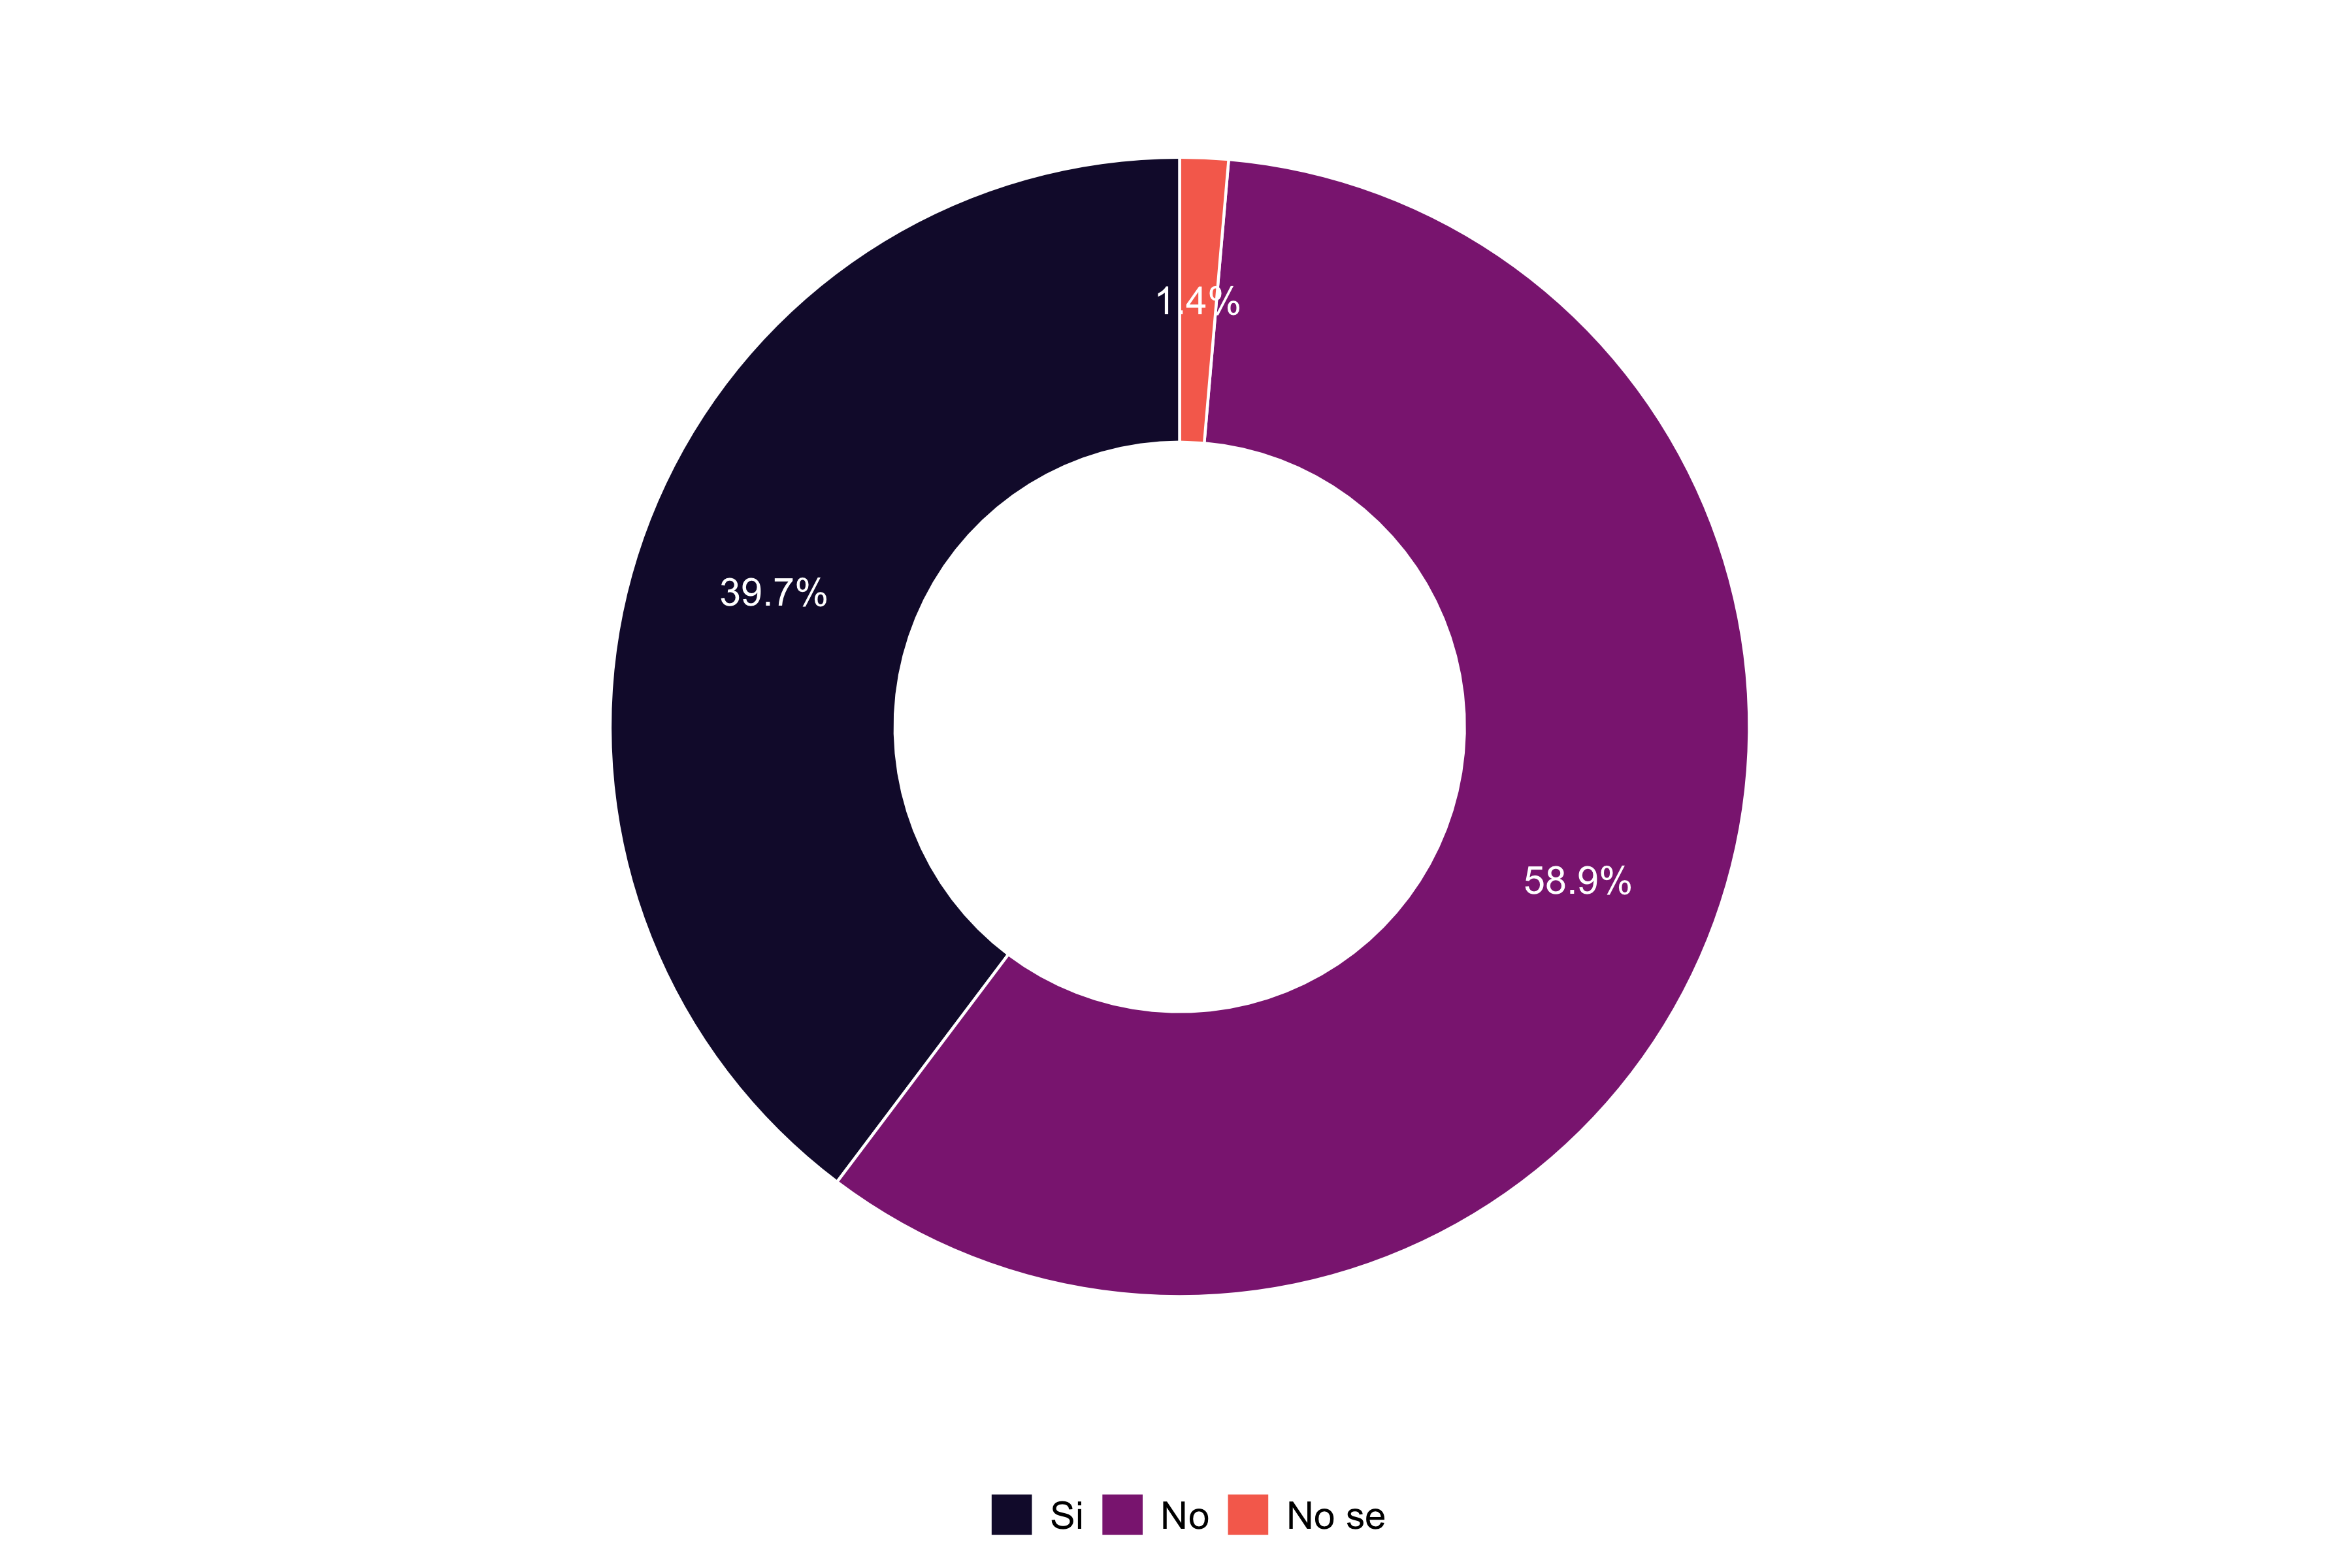
\includegraphics{paper_files/figure-pdf/fig-dona-2-1.png}

}

\caption{¿Ha intentado reproducir resultados de alguien más?}

\end{figure}

\begin{figure}

{\centering 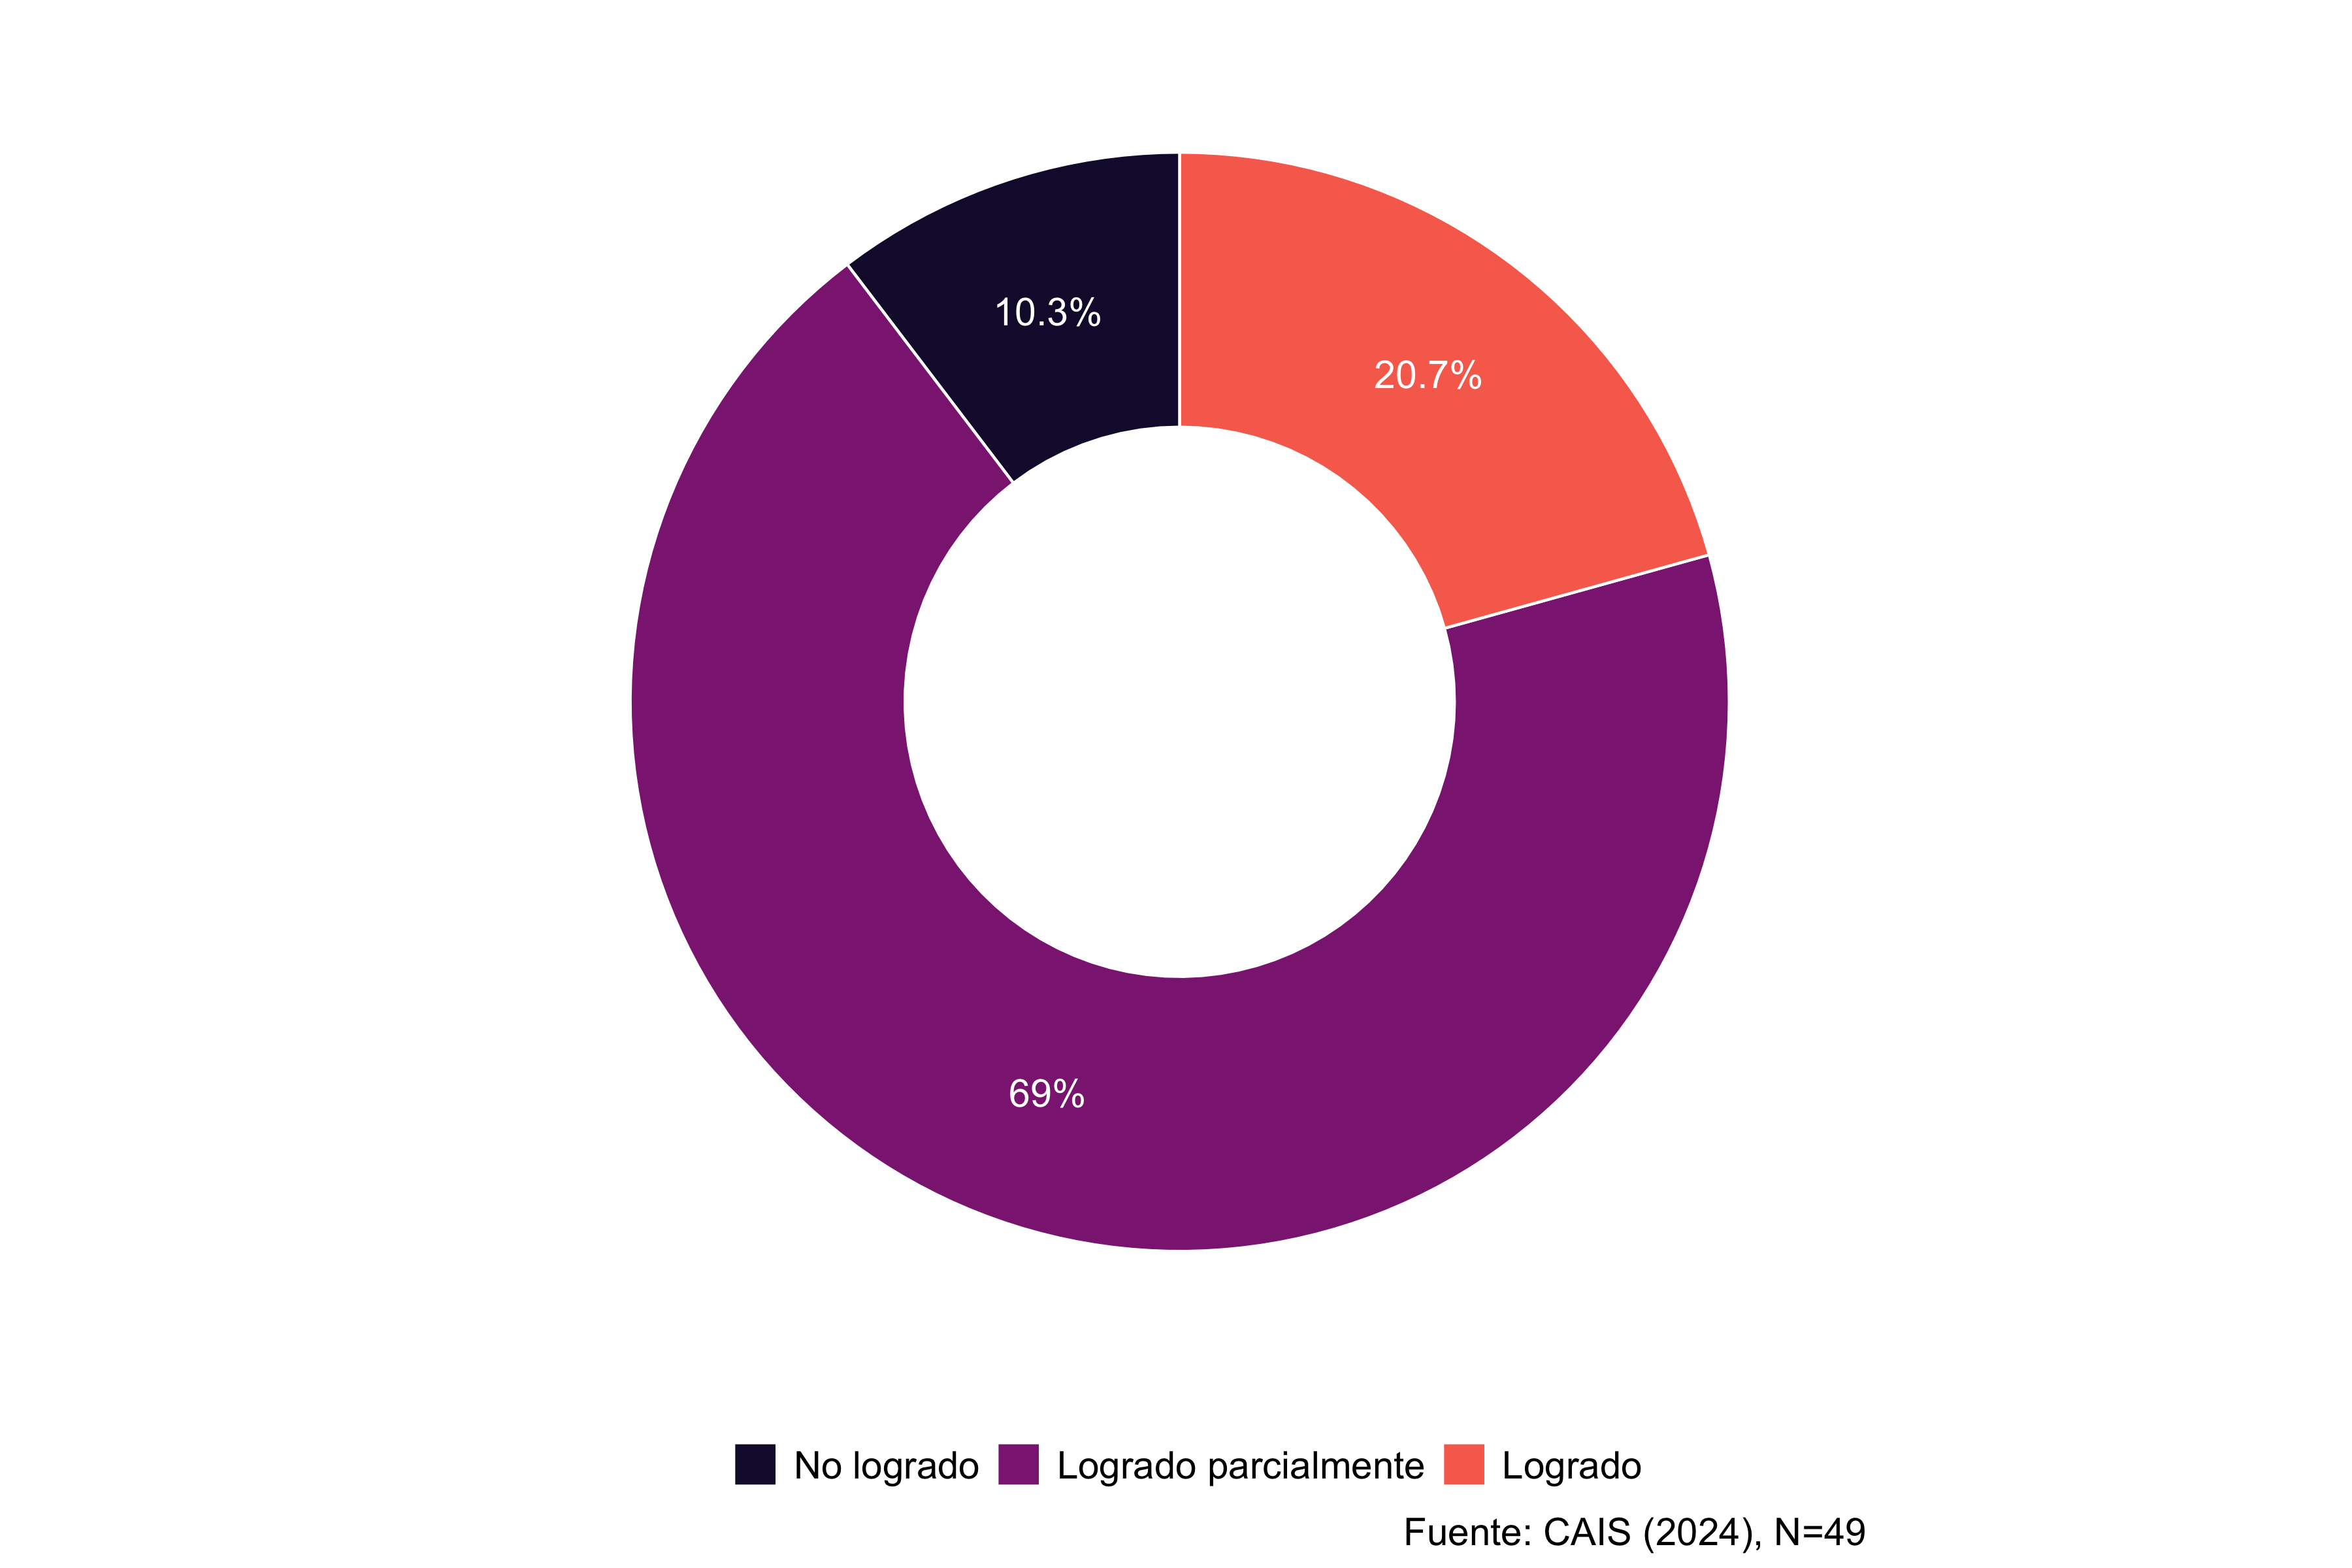
\includegraphics{paper_files/figure-pdf/fig-dona-2-2.png}

}

\caption{De haberlo intentado, ¿En cuál de estas etapas quedó?}

\end{figure}

}

\caption{\label{fig-dona-2}Prácticas asociadas a la reproducibilidad}

\end{figure}

\begin{enumerate}
\def\labelenumi{\alph{enumi})}
\setcounter{enumi}{2}
\tightlist
\item
  Valoraciones Política de Ciencia Abierta de ANID
\end{enumerate}

En primera instancia, la Política de Ciencia Abierta de ANID encuentra
buena acogida entre los encuestados. Así, el 90\% considera que está de
acuerdo o muy de acuerdo con que ANID continúe desarrollando políticas
de ciencia abierta, como se muestra en Figura~\ref{fig-vanid-grid-2-2}.
Asimismo, el 84\% considera bastante o muy necesario la implementación
de políticas de acceso abierto, como se observa en
Figura~\ref{fig-vanid-grid-1}.

\begin{figure}

{\centering 

\begin{figure}

{\centering 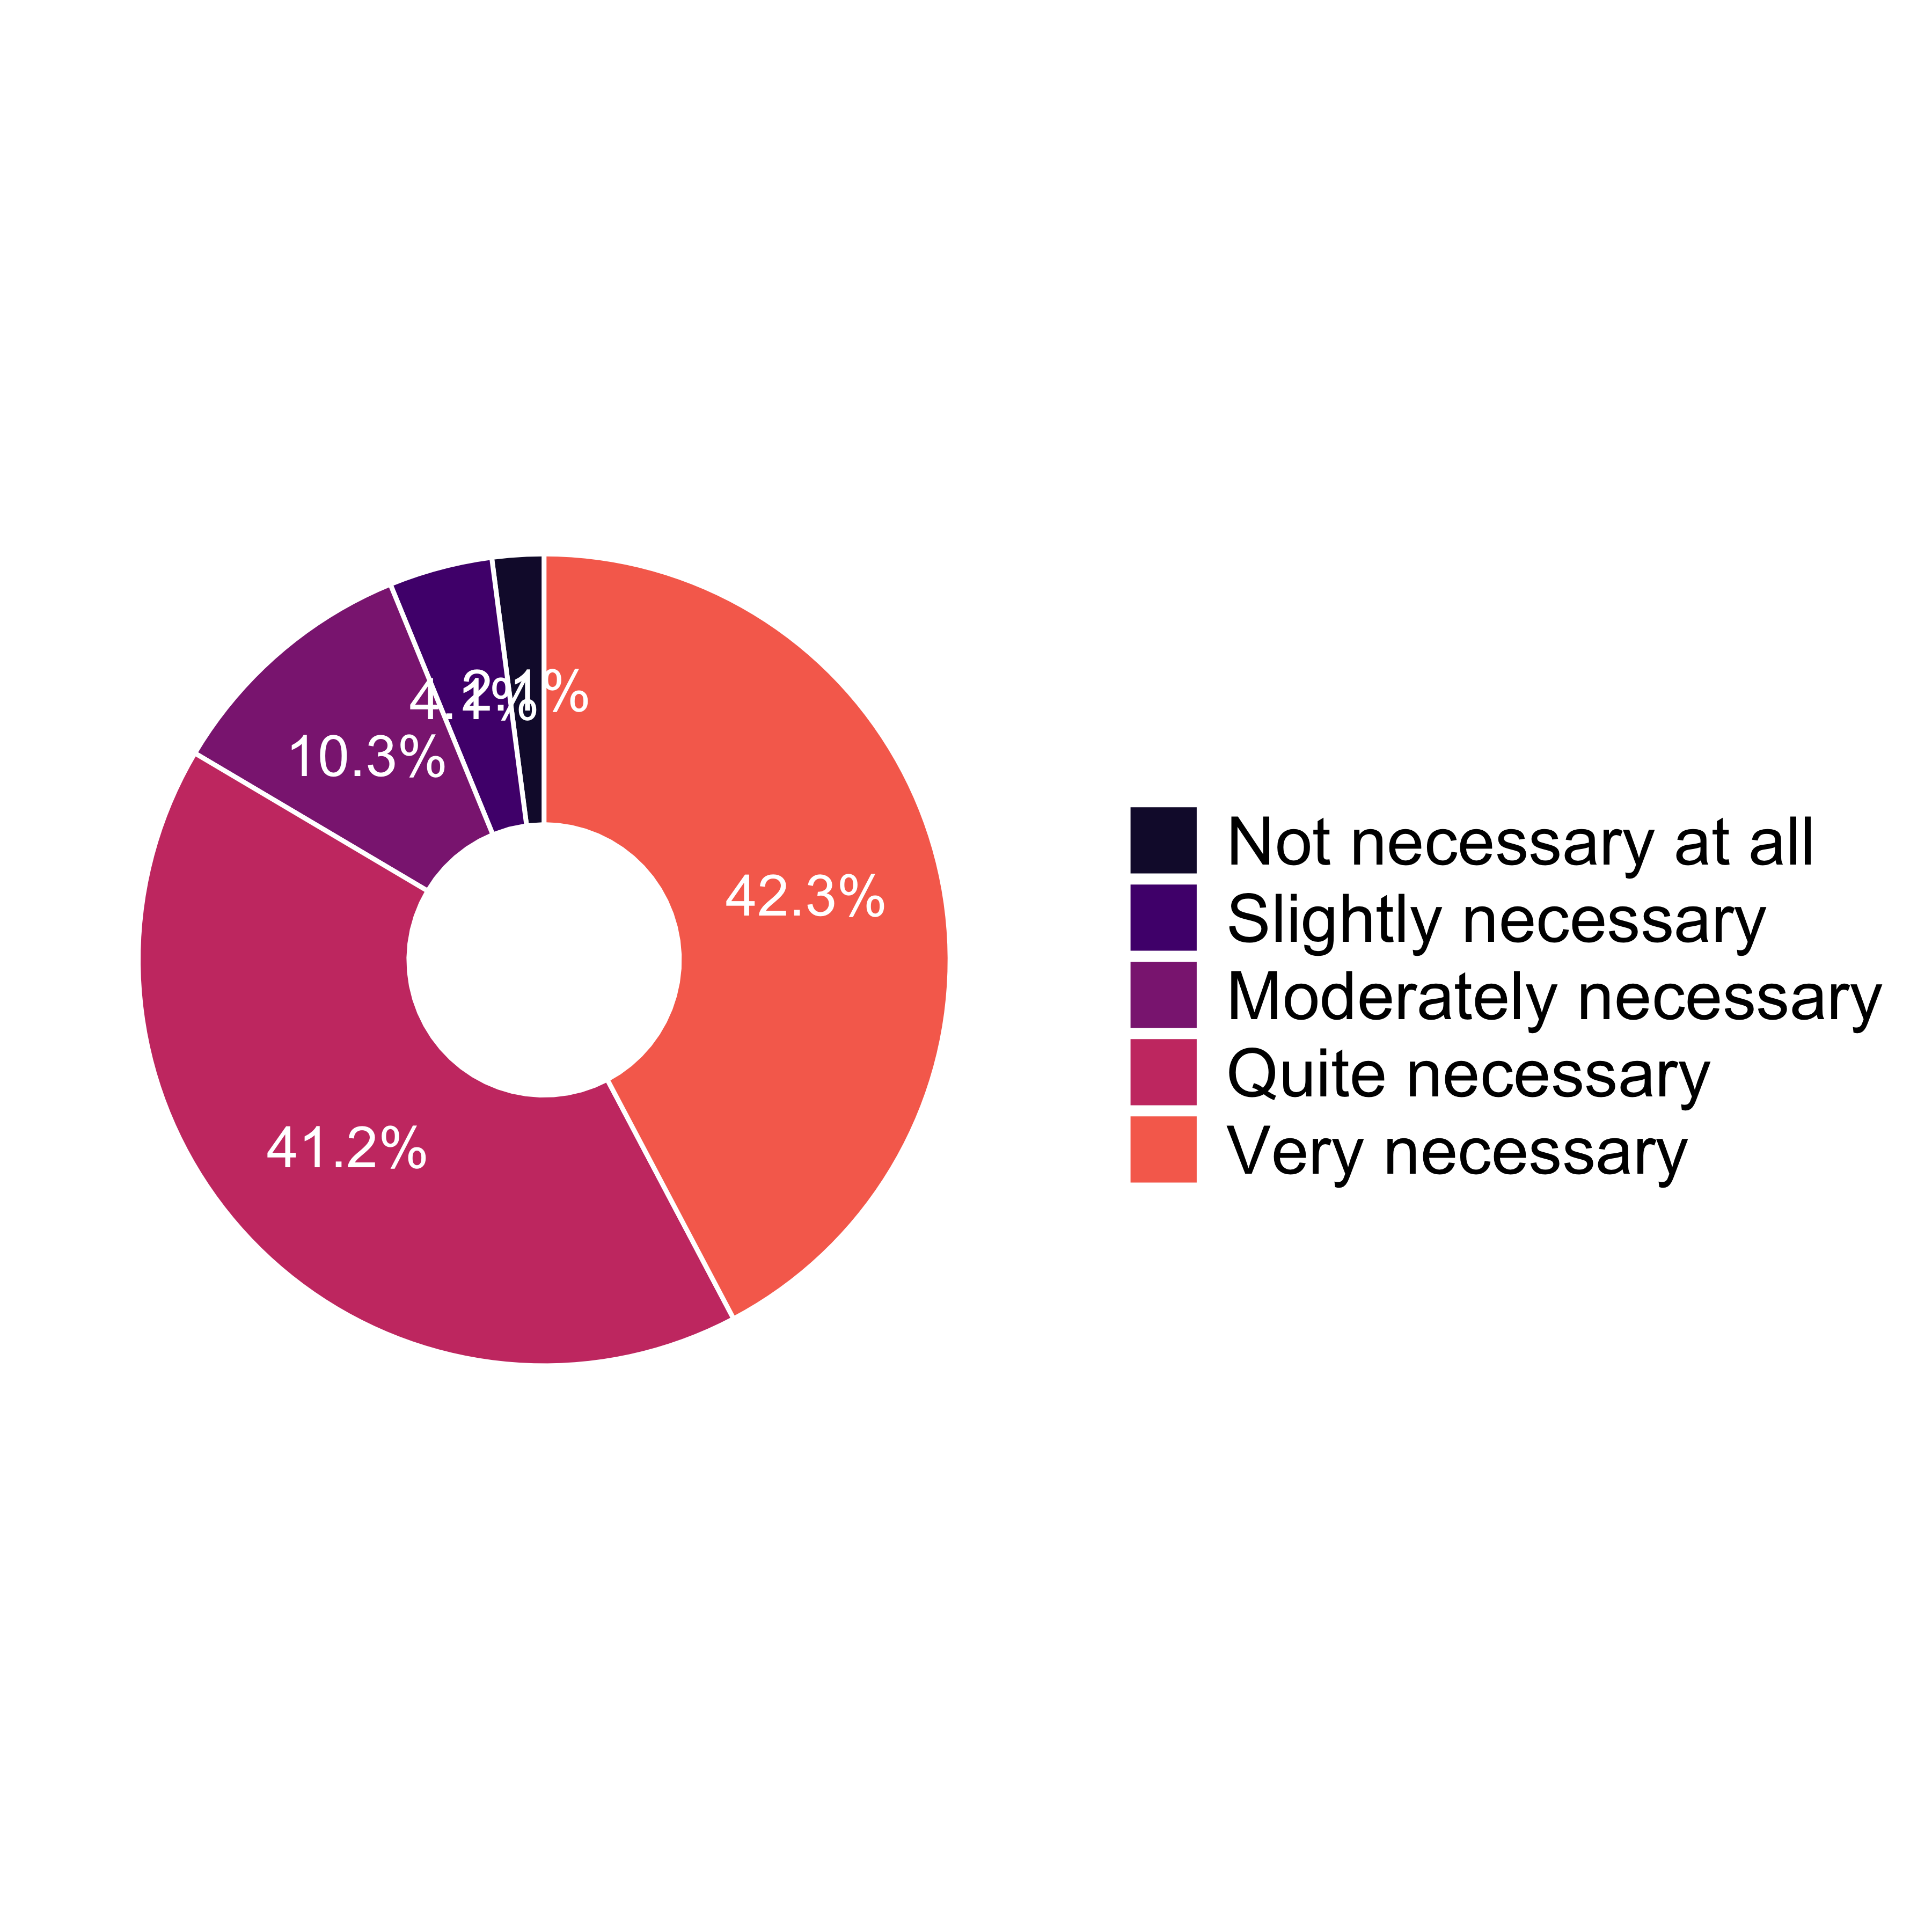
\includegraphics{paper_files/figure-pdf/fig-vanid-grid-1.png}

}

\caption{Qué tan necesario es la implementación de políticas de acceso
abierto obligatorias para investigaciones financiadas por fondos
públicos?}

\end{figure}

\begin{figure}

{\centering 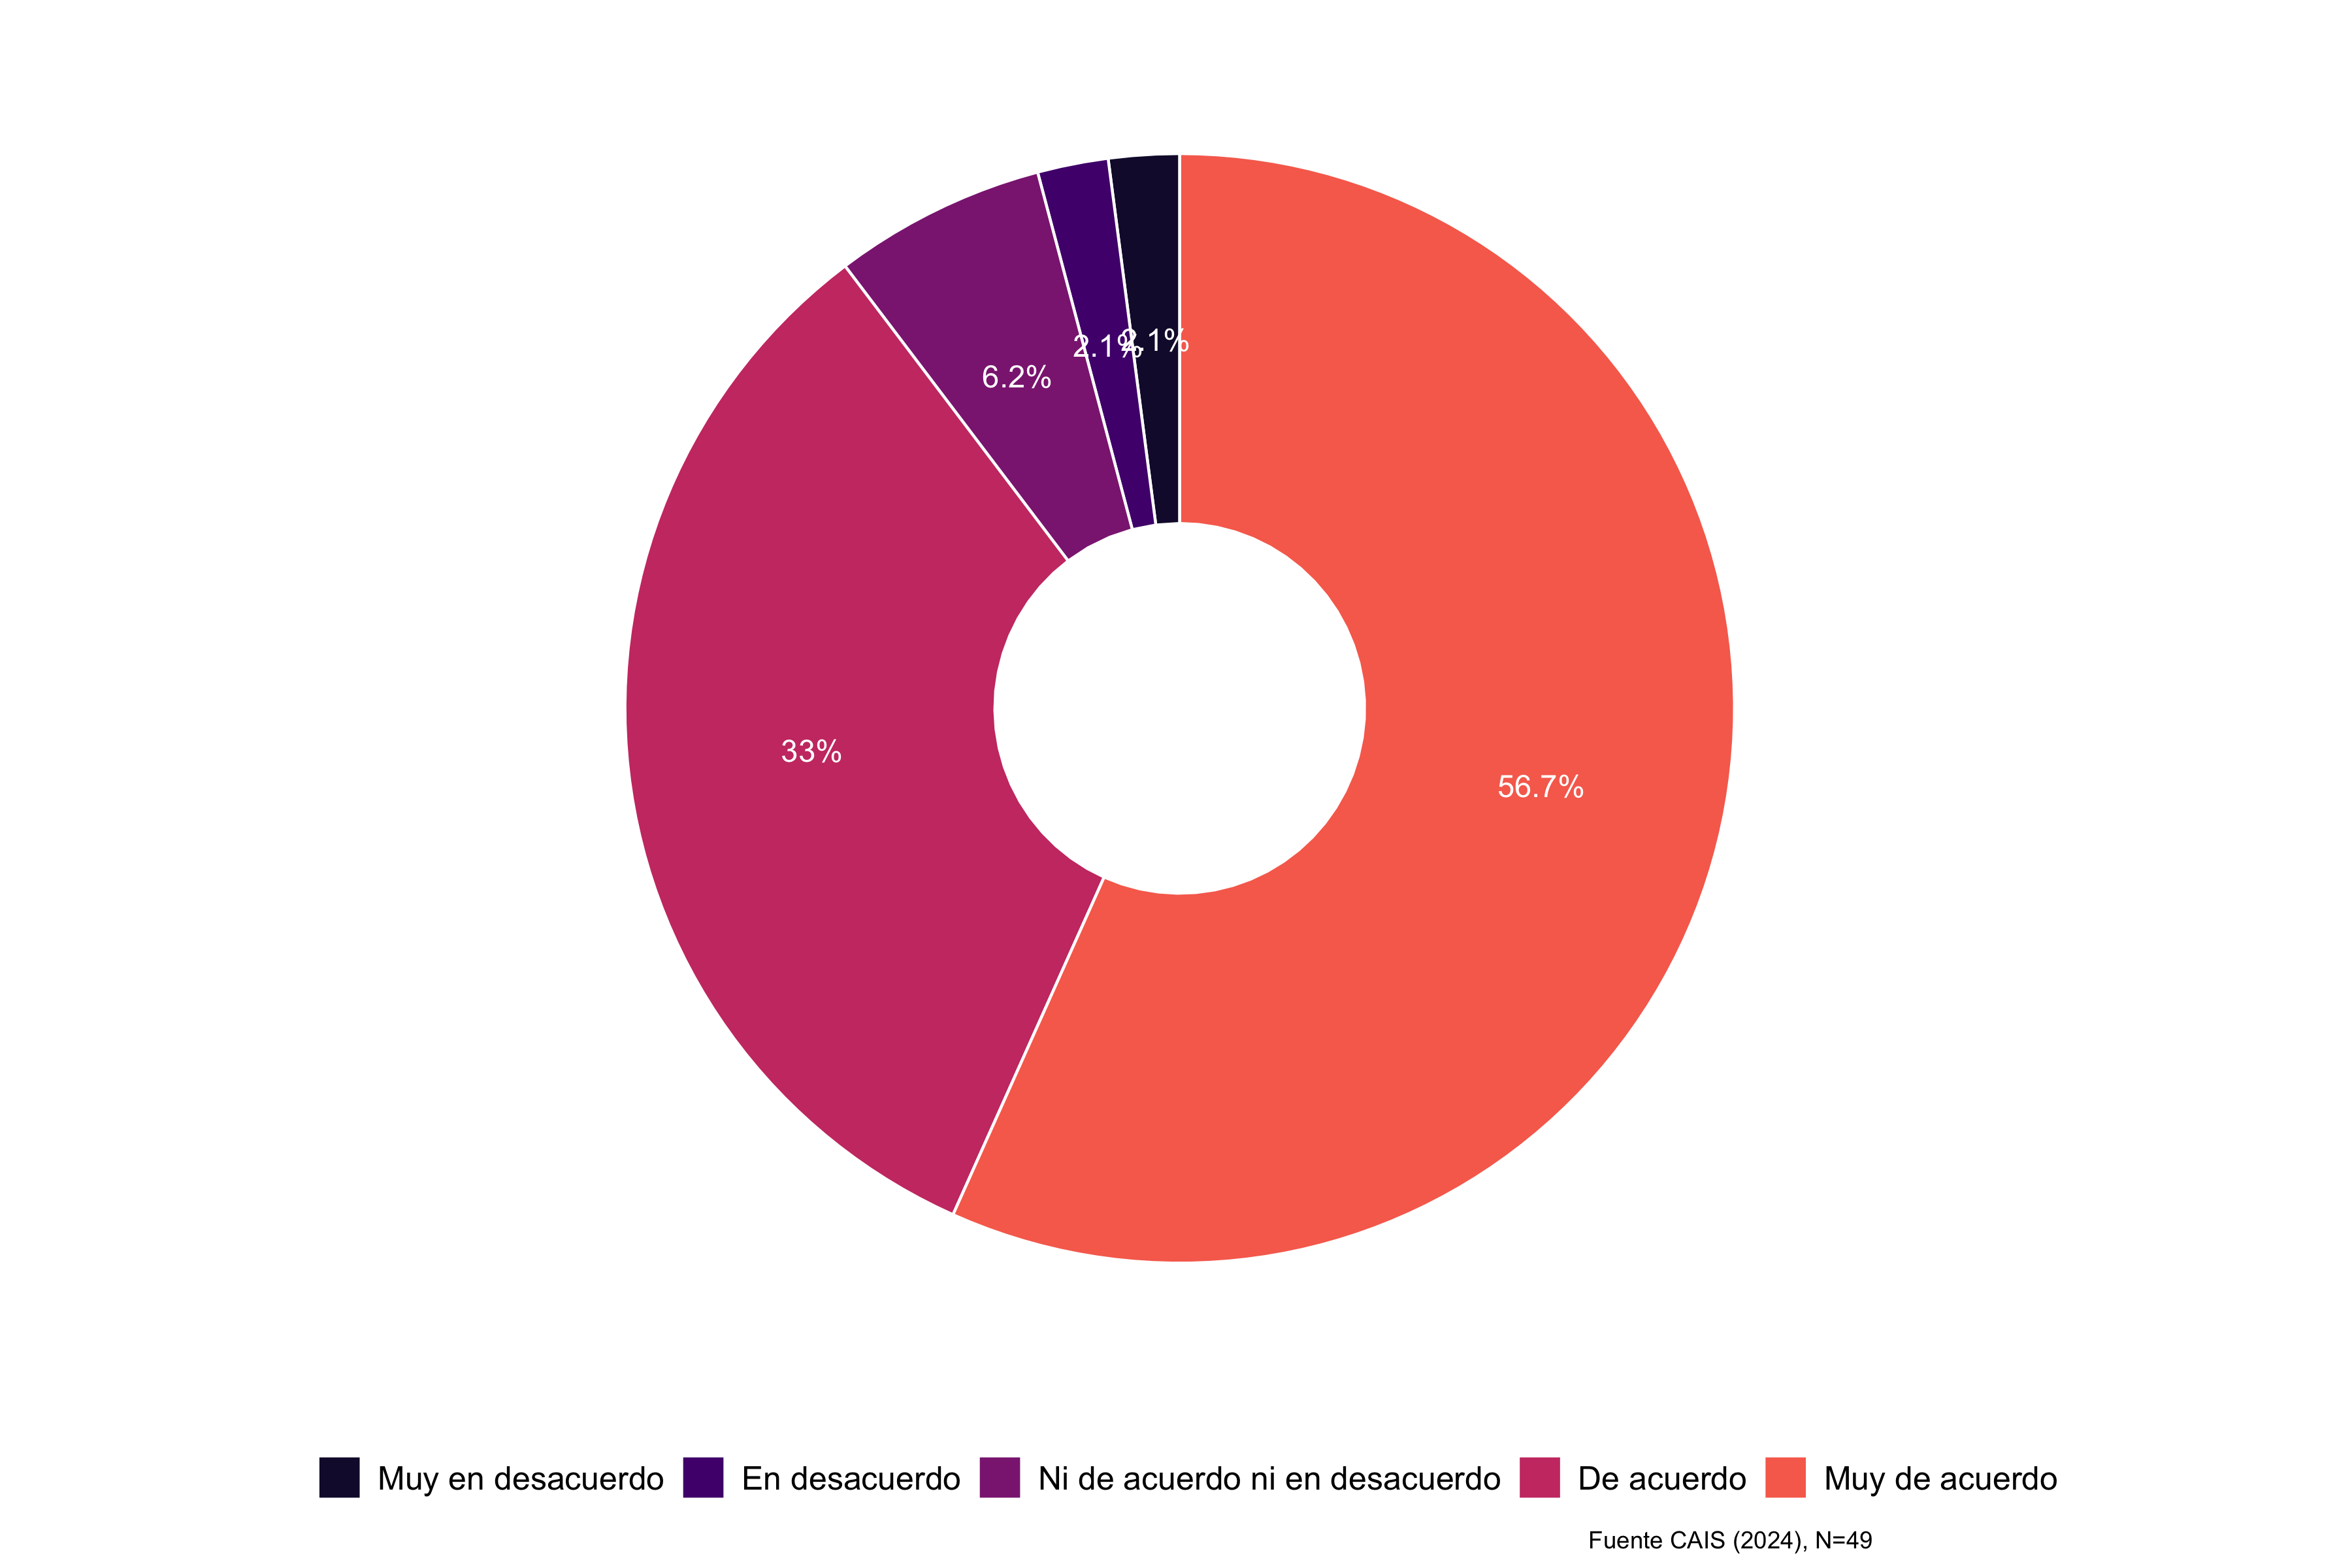
\includegraphics{paper_files/figure-pdf/fig-vanid-grid-2.png}

}

\caption{¿Qué tan de acuerdo se encuentra con que la ANID continúe
desarrollando e implementando políticas de acceso abierto a la
producción científica?}

\end{figure}

}

\caption{\label{fig-vanid-grid}Valoración políticas de ciencia abierta
ANID}

\end{figure}

Sin embargo, hay otras prácticas que encuentran una menor acogida. Así,
tanto la obligatoriedad del prerregistro, como se muestra en
Figura~\ref{fig-vanid-grid-2-1}, como la de la reproducibilidad, como se
observa en Figura~\ref{fig-vanid-grid-2-2}, obtienen el apoyo solo del
50\% de los encuestados.

\begin{figure}

{\centering 

\begin{figure}

{\centering 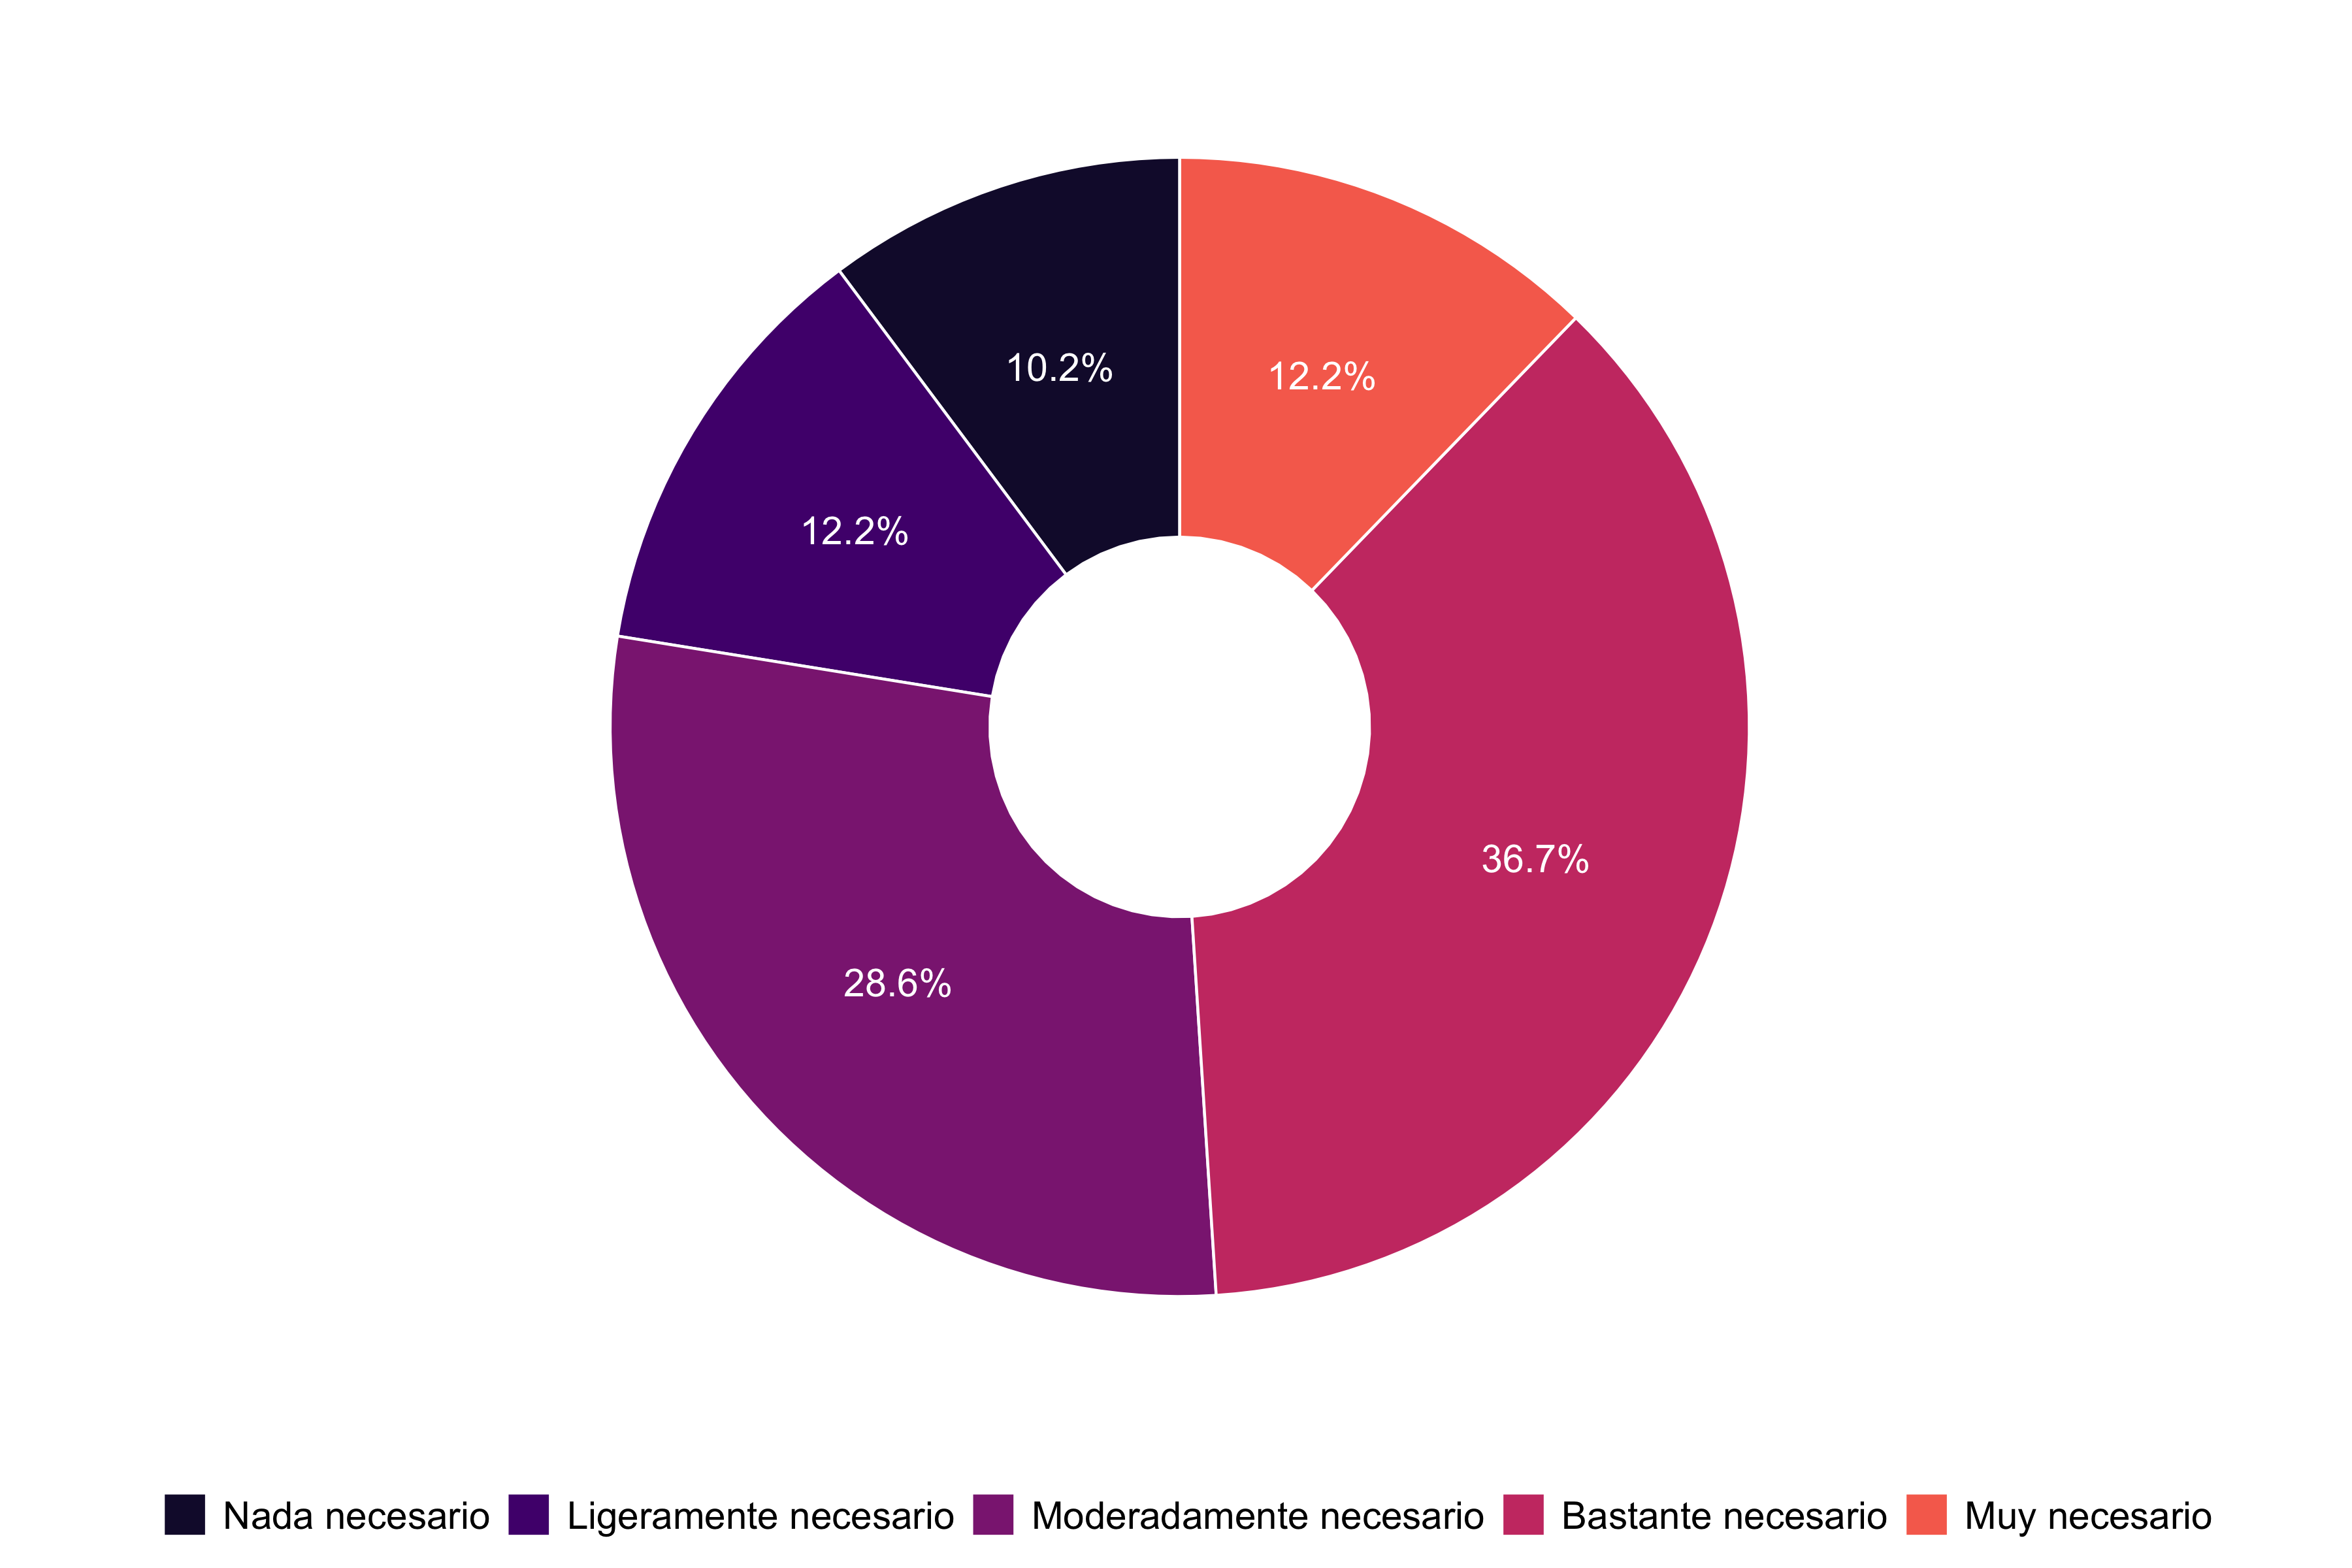
\includegraphics{paper_files/figure-pdf/fig-vanid-grid-2-1.png}

}

\caption{¿Cuán necesario es que la ANID incorpore el pre-registro del
diseño de investigación dentro de su Política de Acceso Abierto?}

\end{figure}

\begin{figure}

{\centering 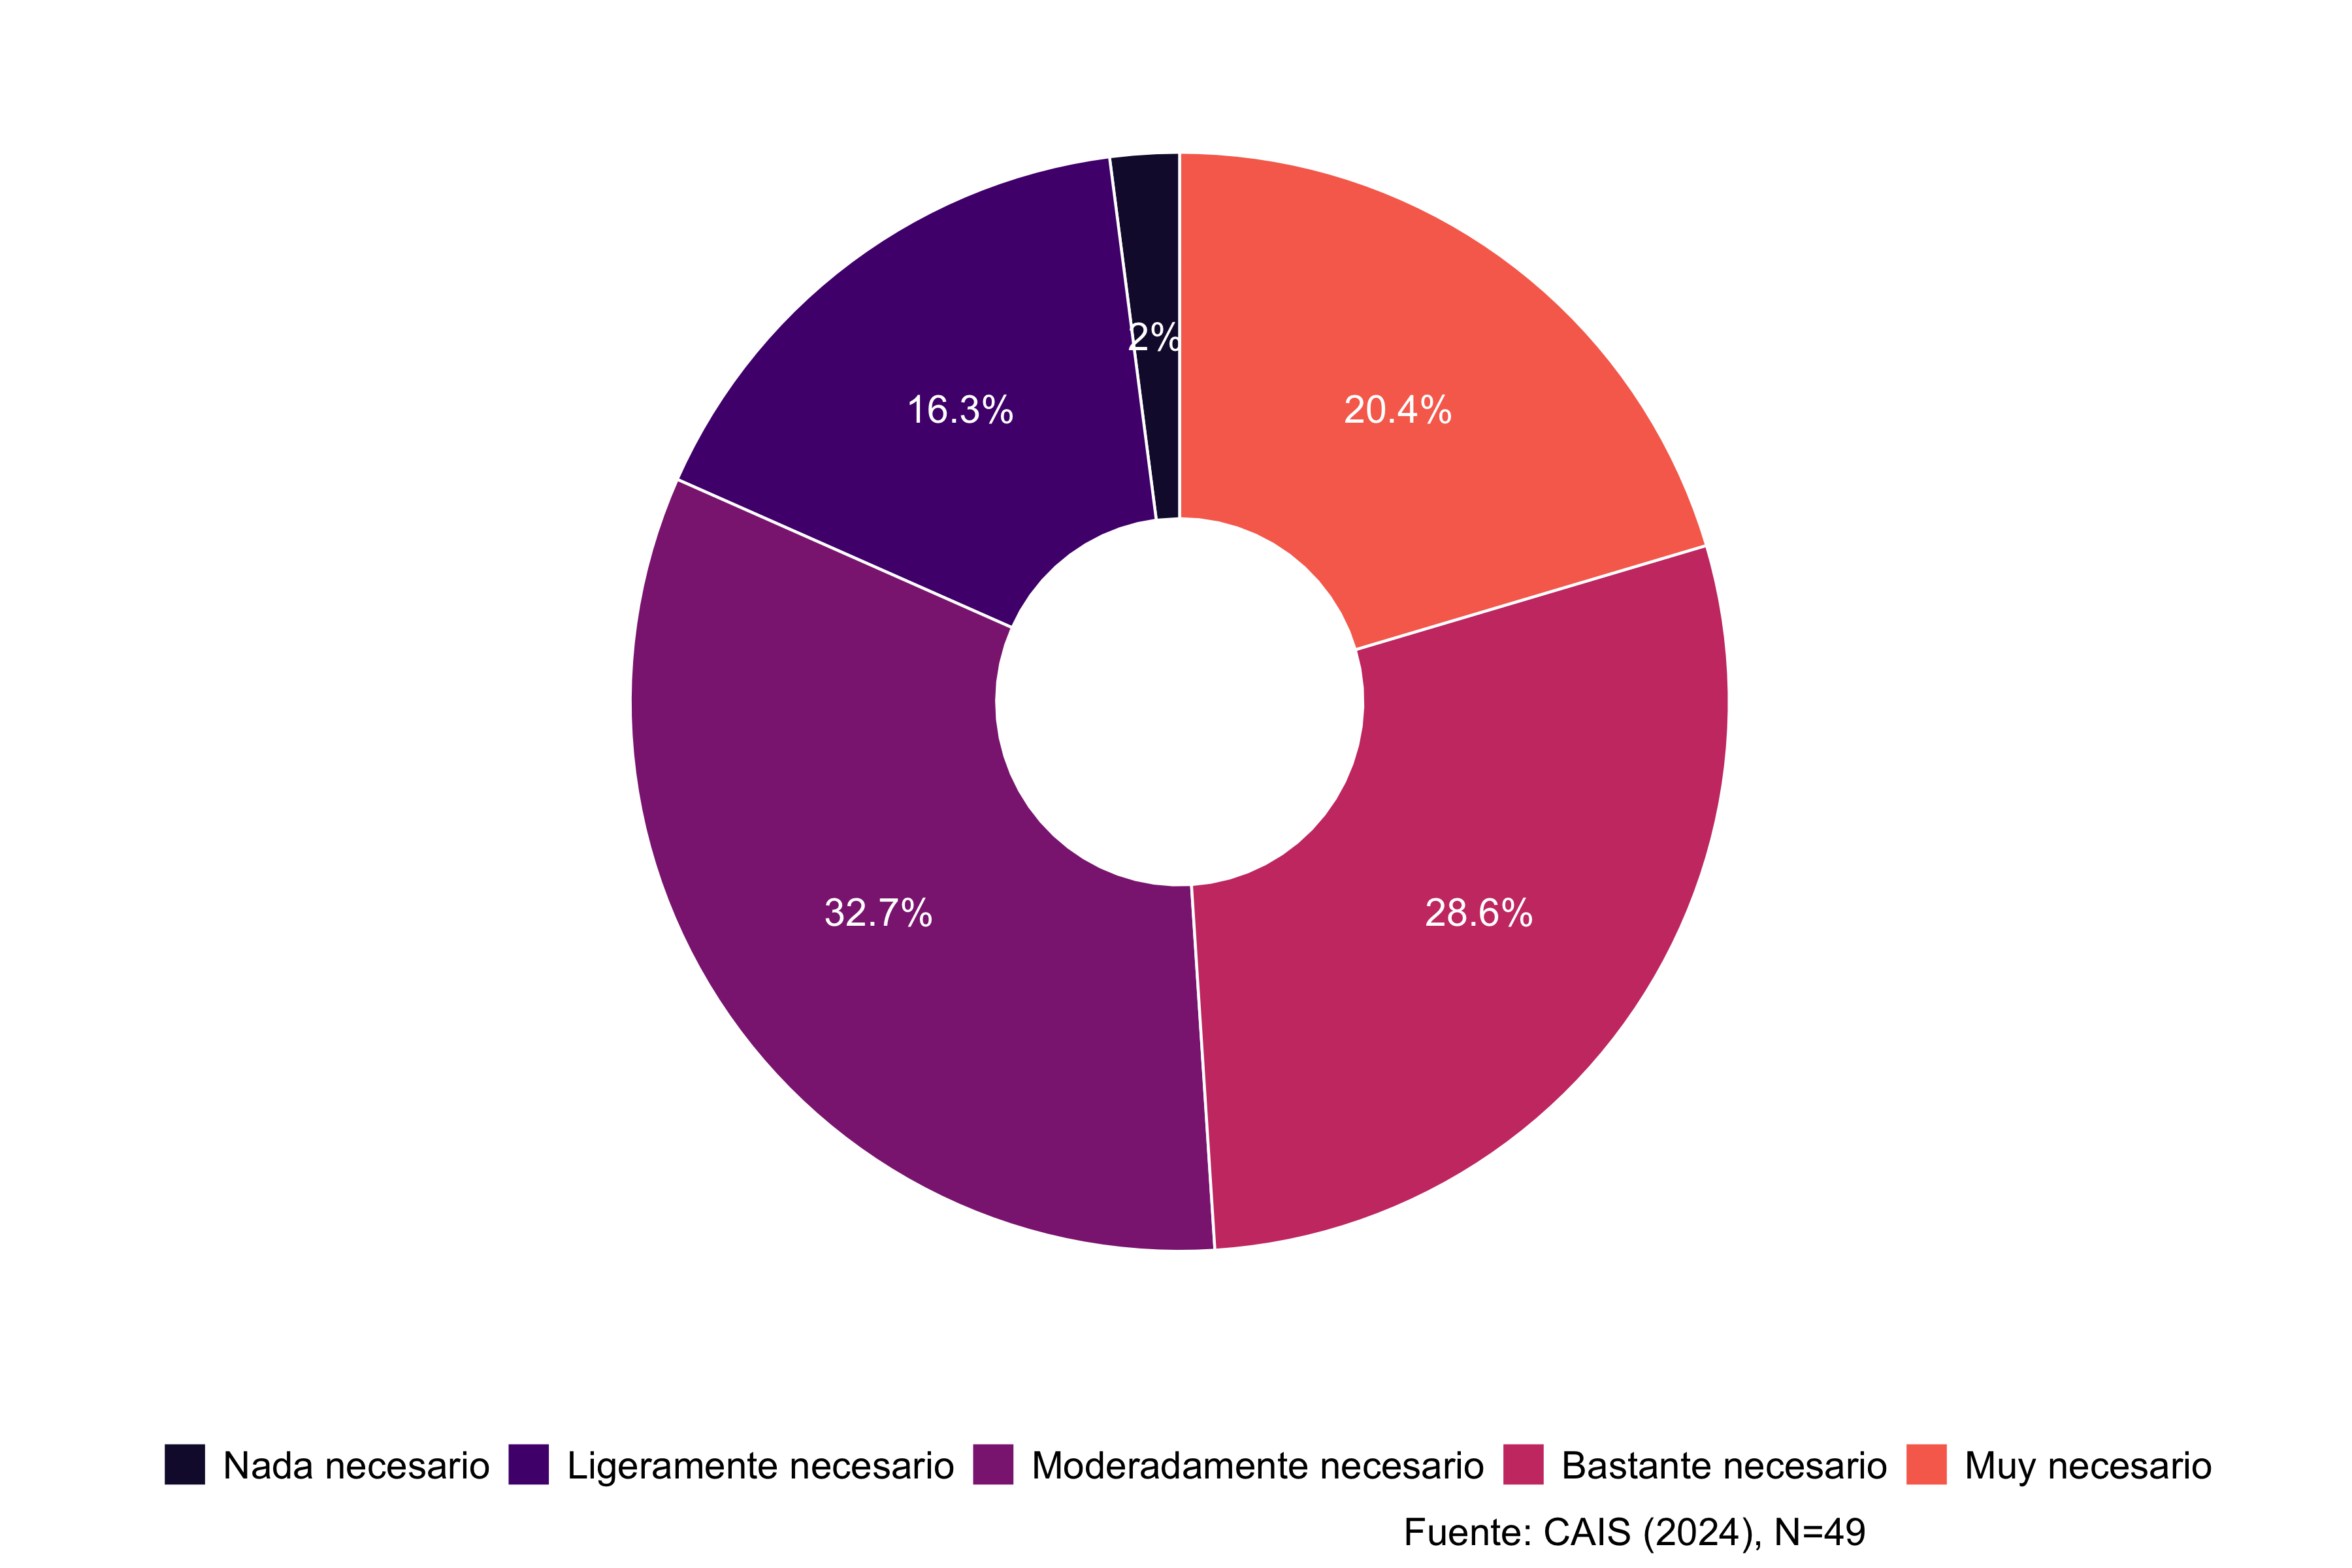
\includegraphics{paper_files/figure-pdf/fig-vanid-grid-2-2.png}

}

\caption{¿Cuán necesario es que la ANID incorpore la reproducibilidad de
la investigación dentro de su Política de Acceso Abierto?}

\end{figure}

}

\caption{\label{fig-vanid-grid-2}Valoración inclusión de prácticas en la
Política de Acceso Abierto de ANID}

\end{figure}

Por último, la política de difusión de la ANID es evaluada negativamente
por la mayoría de los encuestados. Solo un 24\% considera que esta
política es buena o muy buena, como se observa en
Figura~\ref{fig-vanid-2}.

\begin{figure}

{\centering 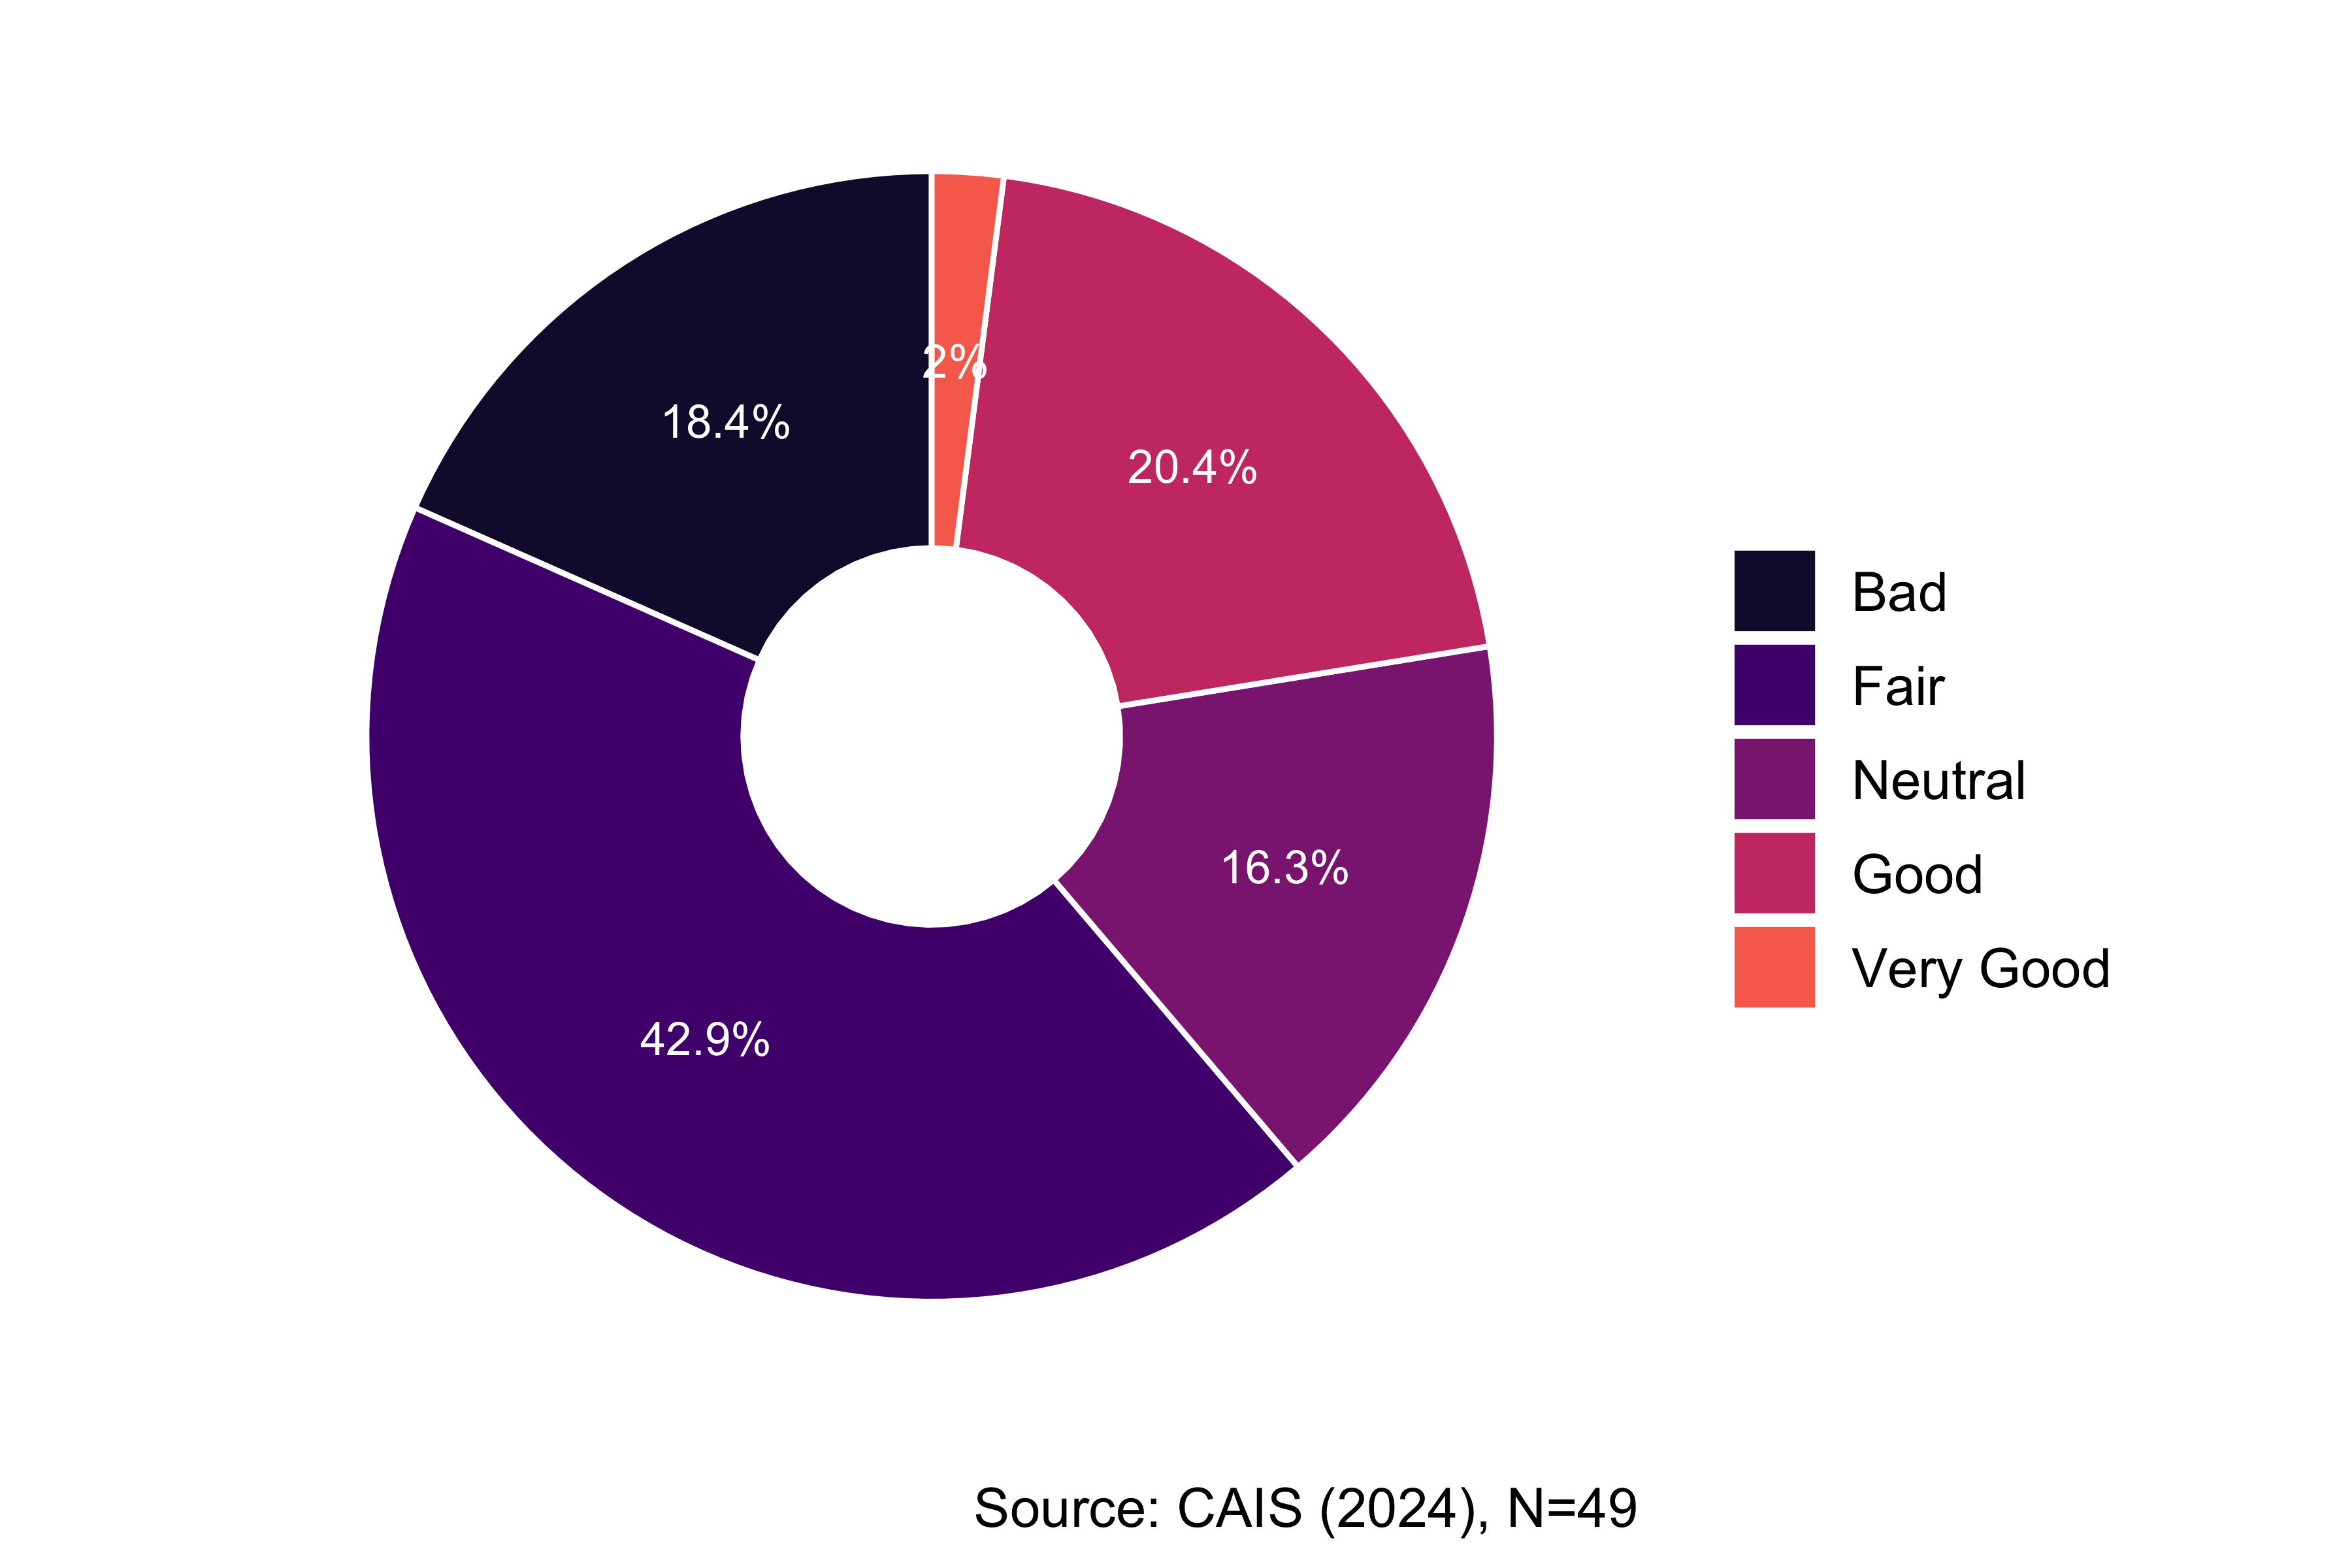
\includegraphics{paper_files/figure-pdf/fig-vanid-2-1.png}

}

\caption{\label{fig-vanid-2}¿Cómo evalúa la difusión de la Política de
Acceso Abierto a la Información Científica y a Datos de Investigación
por parte de la ANID?}

\end{figure}

\hypertarget{discusiuxf3n}{%
\chapter{Discusión}\label{discusiuxf3n}}

\hypertarget{bajo-conocimiento-pocas-pruxe1cticas.}{%
\section{Bajo conocimiento, pocas
prácticas.}\label{bajo-conocimiento-pocas-pruxe1cticas.}}

Ambos estudios apuntan a un niveles medios o bajos de conocimiento de
conceptos relacionados a la ciencia abierta, y niveles aún más bajos de
prácticas. El concepto es asociado, principalmente, a la apertura de
resultados. Ahora bien, el estudio cualitativo apunta a que ésta no se
entiende únicamente como publicación en revistas de acceso abierto, sino
también a otras formas de vincularse con la comunidad y de generar
impacto --- entendido más allá de las métricas de las revistas
académicas.

Esto, además, se encuentra relacionado a una serie de prácticas que
apuntan a la apertura y la transparencia de los resultados de
investigación. Así, en el estudio cualitativo fue posible observar
recuentos de experiencias en publicaciones de acceso abierto, uso de la
``Ruta Dorada'' y compartir artículos o pre-prints mediante redes
sociales o privadas.

Ahora bien, los niveles de conocimiento y prácticas bajan
sustancialmente en lo relativo a conceptos y medidas relacionadas al
diseño transparente, la apertura de datos y la transparencia de
análisis. En general, el estudio cuantitativo parece distinguir que hay
grupos de investigadores que muestran mayores niveles de conocimiento y
prácticas, particularmente los investigadores más jóvenes y aquellos
cuyo enfoque predominante es cuantitativo.

El bajo nivel de conocimiento es reconocido como una de las principales
barreras para llevar a cabo prácticas e implementar medidas concordantes
a los principios de la ciencia. Sin embargo, prácticas relacionadas a la
transparencia del diseño (como los prerregistros de hipótesis), a la
apertura de datos (hacer datos públicos o compartirlos con otros
investigadores), o a la transparencia del análisis (como compartir
códigos de análisis), encuentran muchas más barreras y reticencia por
parte de los investigadores.

\hypertarget{valoraciuxf3n-positiva-general-resquemores-particulares}{%
\section{Valoración positiva general, resquemores
particulares}\label{valoraciuxf3n-positiva-general-resquemores-particulares}}

Como concepto general, la ciencia abierta es vista con buenos ojos. Se
destaca que sus principios permitirían difundir mejor los resultados
entre la comunidad científica, evitando malas prácticas como el
p-harking. Además, aumentaría la posibilidad de generar impacto más allá
de las métricas académicas, facilitando la lectura de los resultados por
parte de las comunidades y los tomadores de decisiones. Esto se conjuga
con una conciencia de que el financiamiento público de las
investigaciones impone cierta responsabilidad de que los resultados y
datos estén abiertos a la comunidad académica y general. Por ello, no
resulta sorpresivo que el 90\% de los encuestados estén a favor de que
ANID implemente políticas de acceso abierto.

Sin embargo, una vez que se indagan en prácticas particulares, empiezan
a surgir resquemores respecto a la posibilidad y la conveniencia de
implementar medidas de ciencia abierta relacionadas a la transparencia
del diseño, la apertura de datos y la transparencia en el análisis. Se
identificaron tres nudos fundamentales:

En primer lugar, la \textbf{dificultad de aplicar muchas de estas
medidas en la investigación cualitativa}. Salvo por la apertura de
resultados, la evaluación positiva de prácticas relacionadas a la
ciencia abierta es mayor entre investigadores con enfoque cuantitativo,
y menor entre quienes practican enfoques predominantemente cualitativos.
Esto va en línea con los observado en el primer estudio, donde se
observó como el prerregistro de hipótesis y la apertura de datos generan
importantes choques a nivel epistemológico, metodológico y ético con los
principios tradicionales de la investigación cualitativa. Del mismo
modo, la crisis de reproducibilidad aparece como una preocupación mucho
mayor entre los investigadores cuantitativos, en línea con lo observado
en el primer estudio, donde se aprecia que la reproducibilidad apenas
aparece en el horizonte de los investigadores cualitativos.

En segundo lugar, la \textbf{dificultad de conciliar los principios de
la ciencia abierta con los imperativos de productividad académica}
impuestos por universidades y agencias públicas. Incluso la apertura de
resultados, el principio con mayor legitimidad, debe enfrentar la
dificultad de que la estructura de financiamiento y las políticas de
difusión de ANID favorecen la publicación en revistas con barreras de
pago. Por otro lado, medidas como el prerregistro y la apertura de datos
levantan suspicacias sobre la protección de la propiedad intelectual de
los investigadores, y que limitan la originalidad y el impacto de
futuras publicaciones.

Por último, se observaron \textbf{reticencias hacia las motivaciones}
detrás de la implementación de estas medidas. Para algunos
investigadores, estas prácticas estarían lejos de escapar de las
criticadas lógicas de difusión y financiamiento. Por ejemplo, se
argumenta que compartir resultados y datos reporta beneficios
personales, mediante el aumento citas, en consonancia a las exigencias
de productividad académica.

En esa línea, el estudio cuantitativo apunta a que efectivamente
construir redes y mejorar la visibilidad están entre las principales
motivaciones para la apertura de datos, especialmente entre
investigadores mujeres y de trayectorias académicas intermedias. Más
allá de cualquier juicio moral sobre las motivaciones de estos
investigadores, resultaría interesante indagar porque hay grupos
específicos que estarían más inclinados a aceptar medidas de ciencia
abierta por razones extrínsecas.

\hypertarget{valoraciuxf3n-cruxedtica-de-la-poluxedtica-de-difusiuxf3n-de-la-anid.}{%
\section{Valoración crítica de la política de difusión de la
ANID.}\label{valoraciuxf3n-cruxedtica-de-la-poluxedtica-de-difusiuxf3n-de-la-anid.}}

Tanto en el estudio cualitativo como en el cuantitativo se pudo apreciar
una percepción crítica hacia las políticas de difusión y de acceso
abierto de la ANID. Principalmente, se observa una tensión entre la
necesidad de transparencia e impacto en la comunidad de investigaciones
financiadas con recursos públicos, y el esquema de financiamiento de
ANID que favorece la publicación en revistas que, por lo general,
presentan barreras de pago.

Los investigadores asocian esto a dos problemas Por un lado, se percibe
que limita la posibilidad real de impacto de las investigaciones,
alejando sus resultados de las comunidades y de los tomadores de
decisiones. Por otro lado, se pone en relieve que este esquema resulta
en el uso de grandes cantidades recursos públicos para financiar el
negocio de grandes compañías editoriales científicas del primer mundo.

\hypertarget{conclusiuxf3n}{%
\chapter{Conclusión}\label{conclusiuxf3n}}

Los estudios aquí presentados apuntan que, para la comunidad de las
ciencias sociales en Chile, la ciencia abierta está asociada
fundamentalmente al acceso abierto a los resultados de la investigación,
ya sea mediante revistas de acceso abierto o mediante otras formas de
difusión. Esto viene acompañado de una serie de prácticas, así como de
una valoración positivas de estas medidas, y posiciones críticas hacia
las políticas de difusión y financiamiento promovidas por ANID. Pese a
esto, otras dimensiones de la ciencia abierta (el diseño transparente,
la apertura de datos y la transparencia del análisis), presentan menores
niveles de conocimiento, menor frecuencia de prácticas y una evaluación
ambivalente.

Ahora bien, se observaron algunas diferencias entre grupos de
investigadores, particularmente respecto al enfoque de investigación. De
tal modo, investigadores con enfoque cuantitativo declararon mayores
niveles de conocimiento, mayor cantidad y frecuencia de prácticas, mayor
preocupación por la crisis de reproducibilidad y una mayor valoración de
las medidas promovidas por la ciencia abierta. Entre investigadores
cualitativos, en cambio, se observaron mayores reticencias, que van
desde barreras prácticas hasta preocupaciones epistemológicas.

La edad y el género también parecen incidir en el conocimiento,
prácticas y valoraciones hacia la ciencia abierta. Futuras
investigaciones podrían apostar a formular modelos que expliquen
diferencias en las disposiciones hacia la ciencia abierta, así como
distinguir entre motivaciones intrínsecas y extrínsecas para aceptar
este tipo de medidas.

En su conjunto, ambos estudios plantean desafíos importantes para las
ciencias sociales abiertas en Chile. En primer lugar, se plantea la
necesidad de revisar las políticas de financiamiento y de difusión de
ANID para ir en mayor concordancia tanto con las necesidades de los
investigadores como con los principios de la ciencia abierta. Así, las
preocupaciones levantadas por los participantes sobre el destino que se
les da a recursos públicos son de suma relevancia y no pueden ser
ignoradas.

En segundo lugar, los estudios ponen en relieve la necesidad de cerrar
brechas de conocimientos y de incentivos que permitan una mayor apertura
hacia la aplicación de medidas de ciencia abierta en otras dimensiones
además de la apertura de resultados. Esto implica abrir espacios de
debate metodológico y epistemológico que permitan superar los
resquemores observados entre algunos grupos de investigadores,
particularmente aquellos con un enfoque predominantemente cualitativo.

\hypertarget{referencias}{%
\chapter*{Referencias}\label{referencias}}
\addcontentsline{toc}{chapter}{Referencias}

\hypertarget{refs}{}
\begin{CSLReferences}{1}{0}
\leavevmode\vadjust pre{\hypertarget{ref-baker_500_2016}{}}%
Baker, Monya. 2016. {«1,500 Scientists Lift the Lid on
Reproducibility»}. \emph{Nature} 533 (7604): 452-54.
\url{https://doi.org/10.1038/533452a}.

\leavevmode\vadjust pre{\hypertarget{ref-boyatzis_thematic_2010}{}}%
Boyatzis, Richard E. 2010. \emph{Transforming Qualitative Information:
Thematic Analysis and Code Development}. Thousand Oaks, Calif.: Sage.

\leavevmode\vadjust pre{\hypertarget{ref-braun_thematic_2006}{}}%
Braun, Virginia, y Victoria Clarke. 2006. {«Using Thematic Analysis in
Psychology»}. \emph{Qualitative Research in Psychology} 3 (2): 77-101.
\url{https://doi.org/10.1191/1478088706qp063oa}.

\leavevmode\vadjust pre{\hypertarget{ref-breznau_does_2021}{}}%
Breznau, Nate. 2021. {«Does {Sociology Need Open Science}?»}
\emph{Societies} 11 (1): 9. \url{https://doi.org/10.3390/soc11010009}.

\leavevmode\vadjust pre{\hypertarget{ref-chopik_relationship_2020}{}}%
Chopik, William J., Christopher R. Chartier, Lorne Campbell, y M. Brent
Donnellan. 2020. {«Relationship Science and the Credibility Revolution:
{An} Introduction to the First Part of the Special Issue»}.
\emph{Personal Relationships} 27 (1): 132-37.
\url{https://doi.org/10.1111/pere.12312}.

\leavevmode\vadjust pre{\hypertarget{ref-creswell_mixedmethods_2018}{}}%
Creswell, John W, y Vicki L Plano Clark. 2018. \emph{Designing and
{Conducting Mixed Methods Research}}. SAGE Publications.

\leavevmode\vadjust pre{\hypertarget{ref-delikoura_open_2021}{}}%
Delikoura, Eirini, y Dimitrios Kouis. 2021. {«Open {Research Data} and
{Open Peer Review}: {Perceptions} of a {Medical} and {Health Sciences
Community} in {Greece}»}. \emph{Publications} 9 (2): 14.
\url{https://doi.org/10.3390/publications9020014}.

\leavevmode\vadjust pre{\hypertarget{ref-enke_user_2012}{}}%
Enke, Neela, Anne Thessen, Kerstin Bach, Jörg Bendix, Bernhard Seeger, y
Birgit Gemeinholzer. 2012. {«The User's View on Biodiversity Data
Sharing --- {Investigating} Facts of Acceptance and Requirements to
Realize a Sustainable Use of Research Data ---»}. \emph{Ecological
Informatics} 11 (septiembre): 25-33.
\url{https://doi.org/10.1016/j.ecoinf.2012.03.004}.

\leavevmode\vadjust pre{\hypertarget{ref-gross_landscapes_2015}{}}%
Gross, Julia, y John Ryan. 2015. {«Landscapes of {Research}:
{Perceptions} of {Open Access} ({OA}) {Publishing} in the {Arts} and
{Humanities}»}. \emph{Publications} 3 (2): 65-88.
\url{https://doi.org/10.3390/publications3020065}.

\leavevmode\vadjust pre{\hypertarget{ref-hail_reproducibility_2020}{}}%
Hail, Luzi, Mark Lang, y Christian Leuz. 2020. {«Reproducibility in
{Accounting Research}: {Views} of the {Research Community}»}.
\emph{Journal of Accounting Research} 58 (2): 519-43.
\url{https://doi.org/10.1111/1475-679X.12305}.

\leavevmode\vadjust pre{\hypertarget{ref-head_extent_2015}{}}%
Head, Megan L., Luke Holman, Rob Lanfear, Andrew T. Kahn, y Michael D.
Jennions. 2015. {«The {Extent} and {Consequences} of {P-Hacking} in
{Science}»}. \emph{Plos Biology} 13 (3): e1002106.
\url{https://doi.org/10.1371/journal.pbio.1002106}.

\leavevmode\vadjust pre{\hypertarget{ref-hodonu-wusu_malasyan_2020}{}}%
Hodonu-wusu, Noorhidawati, y Abrizah. 2020. {«Malasyan Researches on
Open Data. {The} First National Surven on Awareness, Practices and
Attitudes»}. \emph{Malaysian Journal of Library \& Information Science}
25 (2): 1-20. \url{https://doi.org/10.22452/mjlis.vol25no2.1}.

\leavevmode\vadjust pre{\hypertarget{ref-hollenbeck_harking_2017}{}}%
Hollenbeck, John R., y Patrick M. Wright. 2017. {«Harking, {Sharking},
and {Tharking}: {Making} the {Case} for {Post Hoc Analysis} of
{Scientific Data}»}. \emph{Journal of Management} 43 (1): 5-18.
\url{https://doi.org/10.1177/0149206316679487}.

\leavevmode\vadjust pre{\hypertarget{ref-kerr_harking_1998}{}}%
Kerr, Norbert L. 1998. {«{HARKing}: {Hypothesizing After} the {Results}
Are {Known}»}. \emph{Personality and Social Psychology Review} 2 (3):
196-217. \url{https://doi.org/10.1207/s15327957pspr0203_4}.

\leavevmode\vadjust pre{\hypertarget{ref-knudtson_survey_2019}{}}%
Knudtson, Kevin L., Robert H. Carnahan, Rebecca L. Hegstad-Davies, Nancy
C. Fisher, Belynda Hicks, Peter A. Lopez, Susan M. Meyn, et~al. 2019.
{«Survey on {Scientific Shared Resource Rigor} and {Reproducibility}»}.
\emph{Journal of Biomolecular Techniques : JBT} 30 (3): 36-44.
\url{https://doi.org/10.7171/jbt.19-3003-001}.

\leavevmode\vadjust pre{\hypertarget{ref-lacey_open_2020}{}}%
Lacey, Justine, Rebecca Coates, y Matthew Herington. 2020. {«Open
Science for Responsible Innovation in {Australia}: {Understanding} the
Expectations and Priorities of Scientists and Researchers»}.
\emph{Journal of Responsible Innovation} 7 (3): 427-49.
\url{https://doi.org/10.1080/23299460.2020.1800969}.

\leavevmode\vadjust pre{\hypertarget{ref-lewins2007}{}}%
Lewins, Ann, y Christina Silver. 2007. \emph{Using {Software} in
{Qualitative Research}}. 1 Oliver's Yard,~55 City
Road,~London~England~EC1Y 1SP~United Kingdom: SAGE Publications, Ltd.
\url{https://doi.org/10.4135/9780857025012}.

\leavevmode\vadjust pre{\hypertarget{ref-ljubenkovic_survey_2021}{}}%
Ljubenković, Ana Marija, Ana Borovečki, Marko Ćurković, Bjørn Hofmann, y
Søren Holm. 2021. {«Survey on the {Research Misconduct} and
{Questionable Research Practices} of {Medical Students}, {PhD Students},
and {Supervisors} at the {Zagreb School} of {Medicine} in {Croatia}»}.
\emph{Journal of Empirical Research on Human Research Ethics} 16 (4):
435-49. \url{https://doi.org/10.1177/15562646211033727}.

\leavevmode\vadjust pre{\hypertarget{ref-lopezcardenas_percepciones_2021}{}}%
Lopez Cardenas, Maria, y Enrique Cubero-Castillo. 2021. {«Percepciones y
Pr{á}cticas de La Ciencia Abierta En {Venezuela}. {Un} Acercamiento a La
Cuesti{ó}n»}. \emph{Observador del Conocimiento} 5 (4 -diciemb).

\leavevmode\vadjust pre{\hypertarget{ref-nosek_promoting_2015}{}}%
Nosek, B. A., G. Alter, G. C. Banks, D. Borsboom, S. D. Bowman, S. J.
Breckler, S. Buck, et~al. 2015. {«Promoting an Open Research Culture»}.
\emph{Science} 348 (6242): 1422-25.
\url{https://doi.org/10.1126/science.aab2374}.

\leavevmode\vadjust pre{\hypertarget{ref-nowell2017}{}}%
Nowell, Lorelli S., Jill M. Norris, Deborah E. White, y Nancy J. Moules.
2017. {«Thematic {Analysis}: {Striving} to {Meet} the {Trustworthiness
Criteria}»}. \emph{International Journal of Qualitative Methods} 16 (1):
1609406917733847. \url{https://doi.org/10.1177/1609406917733847}.

\leavevmode\vadjust pre{\hypertarget{ref-pardomartinez_knowledge_2018}{}}%
Pardo Martínez, Clara, y Alexander Poveda. 2018. {«Knowledge and
{Perceptions} of {Open Science} Among {Researchers}---{A Case Study} for
{Colombia}»}. \emph{Information-an International Interdisciplinary
Journal} 9 (11): 292. \url{https://doi.org/10.3390/info9110292}.

\leavevmode\vadjust pre{\hypertarget{ref-peng_reproducibility_2015}{}}%
Peng, Roger. 2015. {«The Reproducibility Crisis in Science: {A}
Statistical Counterattack»}. \emph{Significance} 12 (3): 30-32.
\url{https://doi.org/10.1111/j.1740-9713.2015.00827.x}.

\leavevmode\vadjust pre{\hypertarget{ref-rodriguez_awareness_2014}{}}%
Rodriguez, Julia E. 2014. {«Awareness and {Attitudes} about {Open Access
Publishing}: {A Glance} at {Generational Differences}»}. \emph{The
Journal of Academic Librarianship} 40 (6): 604-10.
\url{https://doi.org/10.1016/j.acalib.2014.07.013}.

\leavevmode\vadjust pre{\hypertarget{ref-rowley_academics_2017}{}}%
Rowley, Jennifer, Frances Johnson, Laura Sbaffi, Will Frass, y Elaine
Devine. 2017. {«Academics' Behaviors and Attitudes Towards Open Access
Publishing in Scholarly Journals»}. \emph{Journal of the Association for
Information Science and Technology} 68 (5): 1201-11.
\url{https://doi.org/10.1002/asi.23710}.

\leavevmode\vadjust pre{\hypertarget{ref-sturmer_earlycareer_2017}{}}%
Stürmer, Stefan, Aileen Oeberst, Roman Trötschel, y Oliver Decker. 2017.
{«Early-{Career Researchers}' {Perceptions} of the {Prevalence} of
{Questionable Research Practices}, {Potential Causes}, and {Open
Science}»}. \emph{Social Psychology} 48 (6): 365-71.
\url{https://doi.org/10.1027/1864-9335/a000324}.

\leavevmode\vadjust pre{\hypertarget{ref-zhu_openaccess_2020}{}}%
Zhu, Yimei. 2020. {«Open-Access Policy and Data-Sharing Practice in {UK}
Academia»}. \emph{Journal of Information Science} 46 (1): 41-52.
\url{https://doi.org/10.1177/0165551518823174}.

\end{CSLReferences}



\end{document}
